% ------------------------------------------------------------------------
% -*-TeX-*- -*-Hard-*- Smart Wrapping
% ------------------------------------------------------------------------
%%% Literature Survey --------------------------------------------------

%\addtolength{\topmargin}{-.875in}
%\addtolength{\textheight}{.875in}
%\footskip
%\nonumchapter{Literature Survey}
\chapter{Riemannian Geometry for Brain-Computer Interfaces}
\label{chap:riem-geom-bci}
\epigraph{The history of science has proved that fundamental research is the lifeblood of individual progress and that the ideas that lead to spectacular advances spring from it.}{--- \textup{Sir Edward Appleton}}

\section{Riemannian Manifold of Symmetric Positive-Definite Matrices}
\label{sec:riemann-manifold}

A $\totd$-dimensional \emph{manifold} $\GenMa$ is a Hausdorff space for which every point has a neighbourhood that is homeomorphic to an open subset of $\Re^\totd$ \citep{jost_riemannian_2011}.
When a tangent space is defined at each point, $\GenMa$ is called a differential manifold. 
A \emph{geodesic} $\gamma$ is the shortest smooth curve between two points, $\P_1$ and $\P_2$. 
The tangent space $T_\P\GenMa$ at point $\P$ is the vector space spanned by the tangent vectors of all geodesics on $\GenMa$ passing through $\P$. 
A \emph{Riemannian} manifold is a manifold endowed with an inner product defined on the tangent space, which varies smoothly from point to point.  %at each point is a finite-dimensional Euclidean space. 

For the rest of this chapter, we will restrict to the analysis of the manifold $\Ma$ of  the $\dc\times\dc$ symmetric positive-definite (SPD) matrices, defined as:
\begin{equation*}
	\label{eq:rm}
  \Ma = \left\{ \P \in  \Re^{\dc\times\dc} : \P = \P^\intercal \text{ and } x^\intercal \P x > 0, \forall x \in \Re^{\dc} \backslash 0 \right\} \ . %\nonumber
\end{equation*}
The tangent space $T_{\P}\Ma$ is identified to the Euclidean space of symmetric matrices:
\begin{equation*}
  \label{eq:sy}
  \Sy = \left\{ \S \in \Re^{\dc\times\dc} : \S = \S^\intercal \right\} \ . %\nonumber
\end{equation*}
The dimension of the manifold $\Ma$, and its tangent space $T_{\P}\Ma$, is $\totd = \dc(\dc+1)/2$.

The mapping from a point $\S_i$ of the tangent space to the manifold is called the exponential mapping $\Exp{\P}(\S_i)$: $T_{\P}\Ma \rightarrow \Ma$ and is defined as:
\begin{equation}
	\label{eq:exp_r}
	\Exp{\P}(\S_i) = \P^{\frac{1}{2}}\Expm(\P^{-\frac{1}{2}}\S_i \P^{-\frac{1}{2}})\P^{\frac{1}{2}} \ .
\end{equation}  
Its inverse mapping, from the manifold to the tangent space is the logarithmic mapping $\Log{\P}(\P_i)$: $\Ma \rightarrow T_{\P}\Ma$ and is defined as:
\begin{equation}
	\label{eq:log_r}
	\Log{\P}(\P_i) = \P^{\frac{1}{2}}\Logm(\P^{-\frac{1}{2}}\P_i \P^{-\frac{1}{2}})\P^{\frac{1}{2}} \ .
\end{equation} 
$\Expm(\cdot)$ and $\Logm(\cdot)$ are the matrix exponential and matrix logarithm respectively.
The computation of these operators is straightforward for SPD matrices of $\Ma$. %for symmetric matrices of $\Sy$. % in $T_{\P}\Ma$ or $\Ma$.  
They are obtained from their eigenvalue decomposition (EVD): 
\begin{displaymath}
  \begin{split}
    \P &= U\, \text{diag}(\ev_1, \dots, \ev_\dc)\, U^\intercal \ , \\
    \Expm(\P) &= U\, \text{diag}(\exp(\ev_1), \dots, \exp(\ev_\dc))\, U^\intercal \ , \\
    \Logm(\P) &= U\, \text{diag}(\log(\ev_1), \dots, \log(\ev_\dc))\, U^\intercal \ ,
  \end{split}
\end{displaymath}
where $\ev_1, \dots, \ev_\dc$ are the eigenvalues and $U$ the matrix of eigenvectors of $\P$.
As any SPD matrix can be diagonalised with strictly positive eigenvalues, $\Logm(\cdot)$ is always defined.
Similarly the square root $\P^{\frac{1}{2}}$ is obtained as:
\begin{equation*}
  \label{eq:sqm}
  \P^{\frac{1}{2}} = U\, \text{diag}(\ev_1^{\frac{1}{2}}, \dots, \ev_\dc^{\frac{1}{2}})\, U^\intercal \ , %\nonumber
\end{equation*}
and is unique. The same goes for $\P^{-\frac{1}{2}}$.

The tangent vector of the geodesic $\gamma(t)$ between $\P_1$ and $\P_2$, where $\gamma(0) = \P_1$ and $\gamma(1) = \P_2$ is defined as:
\begin{equation}
  \label{eq:tan_geo}
  v = \overrightarrow{\P_1 \P_2} = \Log{\P_1}(\P_2) \, . 
\end{equation}

%A Riemannian distance between $\P_1$ and $\P_2$ can thus be defined as~\cite{moakher2005differential}:  
%\begin{equation}
%	\label{eq:dist_r}
%	\distR(\P_1,\P_2) = \|\Logm(\P_1^{-1}\P_2)\|_F = \left[\sum_{\chI=1}^{\dc}\log^{2}\lambda_{\chI}\right]^{1/2} ,
%\end{equation}
%where $\lambda_\chI$, $\chI = 1, \dots, \dc$, are the eigenvalues of $\P_1^{-1}\P_2$.
%From Eq.~\eqref{eq:dist_r}, the geometric mean of $\Nb$ points $\P_\nb$ on the manifold, $\nb = 1, \dots , \Nb$, can be defined as the point that minimizes the sum of squared distances to all $\P_\nb$:
%\begin{equation}
%\label{mean_r}
%\Rm(\P_1, \dots, \P_\Nb) = \argmin_{\P \in \Ma} \sum_{\nb=1}^{\Nb} \distR^2(\P_\nb,\P) \ .
%\end{equation}
%%\|\log(P_k^{-1}P)\|_F^2
%This mean has no closed form, and can be computed iteratively \cite{fletcher2004principal}.
%%Syl: was "This geometric mean" but it could be interpreted as a mean of the product of the terms, that is called a geometric mean.

\section{Covariance Matrix Estimation}
\label{sec:covmat-estimation}

When working with covariance matrices, a crucial point is to correctly estimate the covariance when the number of samples is small or heavily corrupted by noise. 
Several approaches have been proposed to build the covariance matrices, relying on normalisation or regularisation of the sample covariances. 
To assess the quality of the covariance matrices obtained from EEG samples, a comparative study of these estimators is conducted.

%Let $X \in \Re^{p \times n}$ denotes a sample of random variables, where $p$ is the number of variables and $n$ the number of samples, $X = [\x_1 \x_2 \dots \x_n]$
Let $\x_\si \in \Re^{\dc}$, $\si=1, \ldots, \dt$, denotes a sample of a multichannel EEG trial recorded on $\dc$ electrodes. 
$\dt$ is the trial length. 
Let $\X \in \Re^{\dc\times\dt}$ be the EEG trial such as $\X = [\x_1, \ldots, \x_{\dt} ]$.
Under the hypothesis that all $\dt$ samples $\x_\si$ are randomly drawn from a distribution, it follows that $\boldsymbol{x}$ is a variable of random vectors and its expected vector is $\EX = E\{ \boldsymbol{x} \}$ \citep{fukunaga_introduction_1990}. %Fukunaga page 18
The covariance matrix of the random variable $\boldsymbol{x}$ is defined by $\P = E\{ (\boldsymbol{x} - \EX)(\boldsymbol{x} - \EX)^{\intercal} \}$ and is unknown, thus an estimate $\cov{ }$ should be computed.
% The covariance matrix $\P$ of EEG multichannel recording is usually unknown and an estimate $\cov{ }$ should be computed.
%There are many techniques that are used to an estimate $\cov{ }$. 
The choice of the appropriate estimator is crucial to verify that the obtained covariance matrices fulfil the following properties: they should be accurate, SPD, and well-conditioned.
The last property requires that the ratio between the maximum and minimum singular value is not too large.
Moreover, to ensure the computational stability of the algorithm, the estimator should provide full-rank matrices, and its inversion should not amplify estimation errors. 

\subsection{Sample Covariance Matrix Estimator}

The most usual estimator is the empirical \emph{sample covariance matrix} (SCM), defined as: 
\begin{equation}
  \begin{split}
    \cov{scm} & = \frac{1}{\dt-1} \sum_{\si=1}^{\dt} (\x_\si - \xb)(\x_\si - \xb)^\intercal 
		\\
    & = \frac{1}{\dt-1} \X\left( \eye_\dt -\frac{1}{\dt}\unitary_{\dt} \unitary_{\dt}^\intercal \right) \X^\intercal \ ,
  \end{split}  
\end{equation}
where $\xb \in \Re^{\dc}$ is the sample mean vector $\xb = \frac{1}{\dt} \sum_{n=1}^\dt \x_\si $.
In the matrix notation, $\eye_{\dt}$ is the $\dt\times\dt$ identity matrix and $\unitary_{\dt}$ is the vector $[1, \ldots, 1]$.
The SCM is often normalised as~\citep{fukunaga_introduction_1990}:
\begin{equation}
  \label{eq:nscme}
  \cov{nscm} = \frac{\dc}{\dt} \sum_{\si=1}^{\dt} \frac{(\x_\si - \xb)(\x_\si - \xb)^\intercal }{\sigma_{\x_\si}^2} \ ,
\end{equation}
with the inter-channel variance at time $\si$ defined as $\sigma_{\x_\si}^2 = (\x_\si - \xb)^\intercal (\x_\si - \xb)$. % A VERIFIER! OK
Another normalisation techniques could be used. 

This estimation is fast and computationally simple.
However when $\dc \approx \dt$, the SCM is not a good estimator of the true covariance. 
In the case $\dc > \dt$, the SCM is not even full rank.

\subsection{Shrinkage Covariance Matrix Estimators}

To overcome the shortcomings of SCM, the shrinkage estimators have been developed as a weighted combination of the SCM and a target covariance matrix, which is often chosen to be close to the identity matrix, \textit{i.e.} resulting from almost independent variables of unit variance.
\begin{equation}
	\label{eq:shrink}
	\cov{shrink} = \kappa \tarco +(1-\kappa)\cov{scm} \ ,
\end{equation} 
where $0 \leqslant \kappa < 1$.
This estimator provides a regularised covariance that outperforms the empirical $\cov{scm}$ for small sample size, that is $\dc \approx \dt$. 
The shrinkage estimator has the same eigenvectors as the SCM, but the extreme eigenvalues are modified, \textit{i.e.} the estimator is shrunk or elongated toward the average.

The different shrinkage estimators differ in their definition of the target covariance matrix $\tarco$. 
Ledoit and Wolf~\citep{ledoit_well-conditioned_2004} ($\cov{shrink\_ledoit}$ on Figure~\ref{fig:acc_errorbar}) have proposed $\tarco=\mathit{v}\eye_{\dc}$, with $\mathit{v} = \text{Tr}(\cov{scm})$. 
Blankertz~\citep{blankertz_single-trial_2011} ($\cov{shrink\_blank}$) defines $\tarco$ also as $\mathit{v}\eye_{\dc}$ but with $\mathit{v} = \frac{\text{Tr}(\cov{scm})}{\dc}$. 
Sch\"{a}fer ($\cov{shrink\_schaf}$) proposes several ways of defining $\tarco$ depending on the observed $\cov{scm}$~\citep{schafer_shrinkage_2005}.
%The shrinkage estimator shrinks (or enlarges) the sample covariance matrix toward a more \textcolor{red}{circular covariance}. 
%When $\lambda = 1$, the estimated covariance matrix $\hat{\Sigma}$ does not take into consideration the empirical data; and when $\lambda=0$, $\hat{\Sigma}$ is not regularized. 

%
%\subsection{Ledoit Shrinkage}
%Ledoit and Wolf developed a shrinkage estimator $\hat{\Sigma}$ of the covariance $\Sigma$ as a linear combination of the identity matrix and the sample covariance matrix, $\hat{\Sigma}=\rho_1I+\rho_2\SCM $ that minimizes the expected quadratic loss $E[\| \hat{\Sigma}-\Sigma \|]$. $\rho_1$ and $\rho_2$ are the shrinkage parameters defined by scalar functions of the covariance matrix $\Sigma$. Since estimator $\Sigma$ is unobserved, these parameters are estimated from the empirical covariance matrix $\SCM$ as described in [Ledoit 2004]. 
%\subsection{Sch\"{a}fer Shrinkage}
%Sch\"{a}fer and Strimmer proposed a shrinkage estimator based on Ledoit and Wolf work [Ledoit2003]. Their estimator is a weighted combination of the sample covariance matrix $\SCM$ and an estimated covariance target $\mathbf{T}$: $\hat{\Sigma}=\lambda \mathbf{T}+(1-\lambda)\SCM$. $\lambda$ is taken to be the argument that minimizes the squared error loss function, i.e. the Frobenius norm: $L(\lambda) = \| \hat{\Sigma} - \Sigma \|_F^2$. This estimator offers a systematic way to obtain a regularized $\hat{\Sigma}$ that outperforms the empirical $SCM$ and the theoretical $\mathbf{T}$, based on the knowledge of data.
%\subsection{Blankertz Shrinkage}

\subsection{Fixed-Point Covariance Matrix Estimator}

The fixed-point covariance matrix~\citep{pascal_theoretical_2005} is based on the maximum likelihood estimator $\mle$ which is a solution to the following equation:
\begin{equation}
\label{eq:max_lik}
\cov{fp} = \mle = \frac{\dc}{\dt} \sum_{\si=1}^\dt \left( \frac{(\x_\si - \xb)(\x_\si - \xb)^\intercal }{(\x_\si - \xb)^\intercal  \mle^{-1} (\x_\si - \xb)} \right) \ .
\end{equation}
%where $p$ is the normalization: $p = tr(\cov{scm})$. 
%This equation admits a single fixed point $\hat{\mathbf{M}}_{fp}$ as solution. 
As there is no closed form expression to Eq.~\eqref{eq:max_lik}, it can be written as a function of $\mle$: $\fmle(\mle) = \cov{fp}$.
%\begin{equation}
%\label{eq:max_lik_func}
%\fmle(\mle) = \frac{p}{\dc} \sum_{i=1}^\dt \left( \frac{(\x_i-\xb)(\x_i-\xb)^\intercal }{(\x_i-\xb)^\intercal  \mle^{-1} (\x_i-\xb)} \right) \ .
%\end{equation}
$\fmle$ admits a single \emph{fixed point} $\mle^*$, where $\fmle(\mle^*) = \mle^*$, which is a solution to Eq.~\eqref{eq:max_lik}. 
Using $\mle_{0}:=\cov{nscm}$ as the initial value of $\mle $, it is solved recursively as $\mle_{t} \underset{t \to \infty}{\longrightarrow} \mle^{*}$.

\section{Classification of SSVEP Covariance Matrices}
\label{sec:classification-covmat}
%%%%%%%%%%%%%%%%%%%%%%%%%%%%%%%%%%%%%%%%%%%%%%%%%%%%%%%%%%%%%%
\subsection{Machine Learning Approach for Classification}
\label{subsec:fund_class}

From multiple labelled observations, belonging to two or more classes, and a new unlabelled observation, the classification task objective is to assign to the class whose elements share similar properties with the considered observation.
In this article, we make two hypotheses that are commonly acknowledged in EEG: the data distribution is Gaussian and classes have identical dispersions.
Given labelled observations $\x_i$ drawn from two classes ($y_i = 1$ or $y_i=-1$), a simple classification algorithm consists in assigning a previously unseen observation to the class with the closest mean.
This simple algorithm requires only to define a computable distance and mean. %, that could be computed
Assuming that the observations are embedded into a dot product space, \textit{e.g.} Euclidean space, the mean can be expressed as:
\begin{equation}
c_{+} = \frac{1}{m_{+}} \sum_{ \left\lbrace i|y_i=+1 \right\rbrace } \x_i \ ,
\label{eq:mean_eucl1}
\end{equation}
\begin{equation}
c_{-} = \frac{1}{m_{-}} \sum_{ \left\lbrace i|y_i=-1 \right\rbrace } \x_i \ ,
\label{eq:mean_eucl2}
\end{equation}
where $y_i \in \left\lbrace +1, -1 \right\rbrace$ is the label of the training observation $\x_i$, $m_{+}$ and $m_{-}$ the number of positive and negative observations respectively. 
An unseen observation $\x$ is assigned to the class whose mean is the closest. 
This simple geometric classification framework is the founding principle of more complex algorithms such as support vector machines. 
It can be formulated in terms of the dot product $\left\langle \cdot, \cdot \right\rangle$.
If $c=(c_{+}+c_{-})/2$ is the point lying halfway between $c_{+}$ and $c_{-}$, and $w=c_{+}-c_{-}$ the vector connecting $c_{+}$ to $c_{-}$, the class label $y$ of the unseen observation $\x$ is determined by checking whether the vector $\x-c$ connecting $c$ to $x$ make an angle $\alpha < \pi/2$ with $w$.   
This is expressed as:
\begin{equation}
\begin{split}
y &= \mathrm{sgn} \left\langle (\x-c),w \right\rangle \\
  &= \mathrm{sgn} \left\langle (\x-(c_{+}+c_{-})/2),(c_{+}-c_{-}) \right\rangle \\
  &= \mathrm{sgn} (\left\langle \x,c_{+} \right\rangle - \left\langle \x,c_{-} \right\rangle + b)
\end{split}
\label{eq:classif1}
\end{equation}
where $\mathrm{sgn}$ is the sign function.
The offset $b$ vanishes if class means are equidistant to the origin \cite{scholkopf_learning_2001}.

This thesis focuses on a simple classification scheme, which assigns a previously unseen observation to the class with closest mean.
The observations are considered in a different feature space, through their covariance matrices, which is not usual in signal processing for BCI.
Most approaches favour more or less complex scheme relying on the estimation of covariance matrices, but consider only Euclidean metrics for the practical computations.
The proposed approach is built upon Riemannian metrics and divergences, and their associated mean.
%%%%%%%%%%%%%%%%%%%%%%%%%%%%%%%%%%%%%%%%%%%%%%%%%%%%%%%%%%%%%%

\subsection{Means of Covariance Matrices}
\label{subsec:mean}

%Consider a multivariate variable $\X \in \Re^{\dc \times \dt}$ where $\dc$ is the number of variables and $\dt$ the number of samples, with $C > N $, 
The covariance matrix of $\X$ which can be estimated with the sample covariance estimator as
\begin{equation}
\cov{} = \frac{1}{\dt} \X \X^\intercal
\end{equation}
is symmetric positive-definite (SPD).
Other estimators seen in Section~\ref{sec:covmat-estimation} are also producing SPD matrices. 
%i.e $\P = \P^\intercal \text{ and } x^\intercal \P x > 0, \forall x \in \Re^{\dc} \backslash 0 \ . \nonumber$
The properties of SPD matrices constrain them to a convex cone:
\begin{enumerate}[label=(\roman*)]
\item Symmetry: $\P = \P^\intercal$
\item Positive definiteness: $\x^\intercal \P \x > 0, \forall x \in \Re^{\dc} \backslash 0$
\item Strict positivity of diagonal elements: $\P_{ij} > 0 | i=j, \forall i,j \in \left\lbrace 1, \dots, \dc \right\rbrace$ i.e. positive variance.
\item Cauchy-Schwarz inequalities: $|\P_{ij}| \leq (\P_{ii} \P_{jj})^{1/2}, \forall i,j \in \left\lbrace 1, \dots, \dc \right\rbrace$
\end{enumerate}


The mean of SPD matrices can be computed as a centre of mass:
given a set of covariance matrices $\{\P_\nb\}_{\nb=1,\dots,\Nb}$,
the centre of mass $\Pm$ is the covariance matrix that minimises the dispersion of matrices $\P_\nb$: %variance
\begin{equation}
	\label{eq:mean}
	\Pm = \Rm(\P_1, \dots, \P_\Nb) = \argmin_{\P \in \Ma} \sum_{\nb=1}^{\Nb} \dist^p(\P_\nb,\P) \ ,
\end{equation}
where $\dist^p(\cdot,\cdot)$ can either be a distance ($p=2$) between two matrices, or a divergence ($p=1$). %, \textit{i.e.} a generalization of squared distance.

In the literature, this mean is shown to have a unique solution and is at times designated as the geometric mean, \emph{Cartan mean}, \emph{Frechet mean}, or \emph{Karcher mean} \footnote{This appellation has been recently criticised by Karcher himself \cite{karcher_riemannian_2014}.} \cite{ando2004geometric,lim_matrix_2012}.
%Cartan \cite{cartan_groupes_1929} had shown that a unique solution to \eqref{eq:mean} exists if all $\P_\nb$ lie in a convex ball \citep[see Section 16 of][]{cartan_groupes_1929}. This applies also to closed convex cones.
Depending on the divergence or distance used, different means can be defined from \eqref{eq:mean}. 
Those considered in this study are presented below and summarised in Table~\ref{tab:dist}.

%From Eq.~\eqref{eq:mean}, several means can be defined and those considered in this study are indicated in Table~\ref{tab:dist}.
%We consider the Euclidean distance $\distF$, as a baseline, giving the Arithmetic mean.
%The first considered Riemannian distance is the Log-Euclidean $\distLE$ distance. 
%Its mean is expressed explicitly~\cite{arsigny_geometric_2007}.
%The second is the Affine-Invariant $\distAIRM$~\cite{moakher_differential_2005}, also called AIRM. 
%Unlike the $\distLE$, it does not have an explicit expression for the mean. 
%It could be efficiently computed with the gradient-based iterative algorithm proposed in~\cite{letcher_principal_2004}.
%The two last distances considered in this study are the log-determinant $\alpha$-divergence~\cite{chebbi_means_2012} and the Bhattacharyya distance~\cite{nielsen_matrix_2012}, the later being a special case of the the former with $\alpha=0$.

%\subsection{Distances and divergences} %(CAN BE MOVED WITHIN THE PREVIOUS SECTION)
%\label{subsec:dist_div}
\subsubsection{Distances and Divergences}
Divergences and distances are measures of dissimilarity between two points in a space.
Here the Riemannian space will be considered.
A distance function $\dist:\GenMa \times \GenMa \rightarrow \Re^+$ has the following properties for all $\P_1, \P_2,\P_3 \in \GenMa$:
\begin{enumerate}[label=(\roman*)]
\item $\dist(\P_1, \P_2) \geq 0$  \tab non-negativity
\item $\dist(\P_1, \P_2) = 0 \, \mathrm{iff} \, \P_1 = \P_2$ \tab identity
\item $\dist(\P_1, \P_2) = \dist(\P_2, \P_1)$ \tab symmetry
\item $\dist(\P_1, \P_3) \leq \dist(\P_1, \P_2) + \dist(\P_2, \P_3)$ \tab triangular inequality 
\end{enumerate}
Divergences are very similar to distances with the difference that properties (iii) and (iv) do not have to be satisfied. 
In the context of Covariance matrices, divergences and distances should both induce a Riemannian metric on the manifold of SPD matrices. 

In this work, we consider several existing distances and their associated mean, namely the Euclidean distance, the Harmonic distance \cite{lim_matrix_2012}, the Affine-invariant Riemannian distance~\cite{pennec_riemannian_2006}, the Log-Euclidean distance~\cite{arsigny_geometric_2007}, the Wasserstein distance~\cite{VIL08}, and divergences, such as the Kullback-Leibler divergence~\cite{nielsen_sided_2009}, the S-divergence~\cite{sra_positive_2016}, the $\alpha$-divergence~\cite{nielsen_clustering_2014}, the Bhattacharyya divergence~\cite{chebbi_means_2012}.
%the Log-det divergence~\cite{dhillon_matrix_2007}, 


%%%%%%%%%%%%%%%%%%%%%%%%%%%%%%%%%%%%%%%%%%%%%%%%%%%%%%%%%%%%%%
\subsubsection{Euclidean Distance}
\label{sec:eucl-distance}
The Euclidean distance between two matrices is represented by the Frobenius norm of their difference:
\begin{equation}
\distF(\P_1, \P_2) = \lVert \P_1-\P_2 \rVert _F = \sqrt{ \tr \left( (\P_1-\P_2)^T (\P_1-\P_2) \right) } \ .
\label{eq:dist_eucl}
\end{equation}
In \eqref{eq:mean}, this yields the arithmetic mean:
\begin{equation}
\PmE = \frac{1}{\Nb} \sum_{\nb=1}^{\Nb} \P_\nb \ .
\label{eq:mean_arithmetic}
\end{equation}
The arithmetic mean is drawn from a family of power means \cite{lim_matrix_2012}, defined as:
\begin{equation}
\P_t = \left( \frac{1}{\Nb} \sum_{\nb=1}^{\Nb} \P_\nb^t \right)^{\frac{1}{t}}, \ t \in [-1,+1] \ .
\label{eq:mean_power}
\end{equation}
and could be expressed as $\PmE = \P_{t|t = 1}$. 
From the same family, one can also define the \emph{harmonic} mean as $\PmH = \P_{t|t = -1}$. 

We consider the arithmetic mean $\PmE$, as a baseline. 
This arithmetic mean is not adequate in the space of SPD matrices for two main reasons. 
First, the Euclidean distance and the arithmetic mean does not guarantee invariance under inversion know as \emph{duality}, and thus could not guarantee that a matrix and its inverse are at the same distance from the identity matrix. 
Second, the arithmetic mean of covariance matrices leads to a \emph{swelling effect}: the determinant of the arithmetic mean of SPD matrices can be larger than the determinant of its individual components.
And since the determinant of a covariance matrix is a direct measure of the dispersion of the multivariate variable, the swelling effect introduces a large distortion of the data dispersion~\cite{arsigny_geometric_2007}.
For these reasons, it is more appropriate to rely on a mean that adapt to the geometry of the SPD matrices. 

\subsubsection{Affine-Invariant Riemannian Distance}

The convex cone of SPD matrices is a manifold that can be endowed with a Riemannian metric; such manifolds are called Riemannian manifold.
The affine-invariant Riemannian (AIR) distance between two points is defined by the length of the curve connecting these points on the Riemannian manifold known as the \emph{geodesic}~\cite{pennec_riemannian_2006}. 

Let $\GenMa$ be a Riemannian manifold, and $T_\P\GenMa$ its tangent space defined on the point $\P$. 
A Riemannian metric $\metric$ is a family of inner product defined on the tangent space defined on each point $\P$ of the manifold.
This inner product varies smoothly from point to point on the manifold,
\[
 \metric_\P: T_\P\GenMa\times T_\P\GenMa \rightarrow \Re \]
$\metric$ is a function that assigns, for each point $\P \in \GenMa$, an inner product in the tangent space $T_\P\GenMa$  .
The Riemannian metric allows to compute the length of vectors or distance between two points on the tangent space. 

The affine-invariant Riemannian distance is the distance between two points of a Riemannian manifold and is defined as: 
\begin{equation}
\distAIRM(\P_1, \P_2) = \lVert \Logm(\P_1^{-1/2}\P_2\P_1^{-1/2}) \rVert_F = \left( \sum_{\chI=1}^{\dc} \log^2 \lambda_\chI \right)^{1/2},
\label{eq:dist_air}
\end{equation}
where $\Logm$ is the matrix logarithm and $\lambda_\chI$, $\chI = 1, \dots, \dc$, are the eigenvalues of $\P_1^{-1}\P_2$. %instead of $\log$ for scalars,
This expression is obtained by solving the geodesic equations on the space of SPD matrices. 

Inserting \eqref{eq:dist_air} in \eqref{eq:mean} yields the mean $\PmAIRM$ associated to the affine-invariant Riemannian metric. 
It is the solution to:
\begin{equation}
\sum_{\nb=1}^\Nb \Logm(\PmAIRM^{-1/2} \P_\nb \PmAIRM^{-1/2})=0 \ .
\label{mean_air}
\end{equation}
It has no closed form solution and can be solved iteratively through a gradient descent algorithm \cite{fletcher_principal_2004}. 

This distance and mean are invariant to affine transformations. 
Some of these invariances are particularly interesting for the SPD matrices
Let $f$ be an affine-invariant Riemannian function defined on $\GenMa \times \GenMa$ (e.g. distance or mean), it displays the following properties:
\begin{enumerate}[label=(\roman*)]
\item \emph{Invariance under congruent transformation, for any invertible matrix $W$}
\begin{equation}
f(\P_1, \P_2) = f(W^\intercal \P_1 W, W^\intercal \P_2 W)
\label{eq:invar_congr}
\end{equation}
\item \emph{Invariance under inversion}
\begin{equation}
f(\P,\eye) = f(\P^{-1},\eye)
\label{eq:invar_invers}
\end{equation}
implying self-duality
\begin{equation}
f(\P_1,\P_2) = f(\P_1^{-1},\P_2^{-1})
\label{eq:invar_invers2}
\end{equation}
\end{enumerate}
Another interesting property of the affine-invariant Riemannian metric is its invariance to left- and right-multiplication by a positive matrix \cite{arsigny_geometric_2007}:
\begin{equation}
f(\P_1, \P_2) = f(\P \P_1, \P \P_2) = f(\P_1 \P, \P_2 \P) \ .
\label{eq:invar_mult}
\end{equation}

\subsubsection{Log-Euclidean Distance}
The Log-Euclidean is another distance that takes into consideration the topology of Riemannian manifold. 
It was introduced to alleviate the complexity involved in the computation of the affine-invariant Riemannian distance and its related mean~\cite{arsigny_geometric_2007}. 
The mean associated to the Log-Euclidean distance corresponds to an arithmetic mean in the domain of matrix logarithms.  
The distance between two SPD matrices is expressed as:
\begin{equation}
\distLE(\P_1, \P_2) = \lVert \Logm(\P_1)-\Logm(\P_2) \rVert_F \ ,
\label{eq:dist_LE}
\end{equation}
and its associated mean is defined explicitly:
\begin{equation}
\PmLE = \Expm \left( \frac{1}{\Nb} \sum_{\nb=1}^{\Nb} \Logm(\P_\nb) \right) \ .
\label{eq:mean_LE}
\end{equation}
Unlike the affine-invariant Riemannian mean, the Log-Euclidean mean has a closed form expression, providing a large computational advantage. 
Moreover, the obtained mean is, to a large extent, similar to the affine-invariant Riemannian mean:
\begin{enumerate}[label=(\roman*)]
\item they have the same determinants which correspond to the geometric mean of the determinants of their matrices  \citep{arsigny_geometric_2007}: \[ \det \PmLE = \det \PmAIRM  = \prod_{\nb=1}^{\Nb} (\det \P_\nb)^{1/\Nb} = \exp \left( \frac{1}{\Nb} \sum_{\nb=1}^{\Nb} \log( \det \P_\nb) \right) \ ; \]
\item they are similar, in some cases identical, and if not, $\tr \PmLE > \tr \PmAIRM$ ;
\item Log-Euclidean mean has properties close to affine-invariance, \textit{i.e.} similarity-invariance instead of congruent-invariance.
\end{enumerate}

\subsubsection{Wasserstein Distance}

The Wasserstein distance, also known as the earth mover's distance, is a measure of distance between two probability distributions. It is the optimal cost of moving one probability distribution into another. 
If the two probability distributions are pictured as two different ways of piling up a mass of sand, then the Wasserstein distance can be seen as the optimal cost involved in transporting sand from one piling to another~\cite{VIL08}.

Let $P(\mathcal{X})$ and $P(\mathcal{Y})$ two spaces of probability measures,
the optimal transport between two masses (or probability distributions) $\eta \in P(\mathcal{X})$ and $\nu \in P(\mathcal{Y})$ is defined as~\cite{VIL08}:
\begin{equation}
C(\eta, \nu) = \inf_{\pi \in \Pi(\eta,\nu)} \int c(x,y) d \pi(x,y) \ ,
\label{eq:opttrans}
\end{equation}
where $\Pi(\eta, \nu)$ is the set of all joint probabilities on $\mathcal{X} \times \mathcal{Y}$; and $c(x,y)$ is the cost for transporting one unit of mass from $x$ to $y$.
In the Wasserstein distance, the cost $c(x,y)$ is defined as a distance. 
The Wasserstein distance of order $p$ is defined as:
\begin{equation}
W_p(\eta,\nu) =  \left( \inf_{\pi \in \Pi(\eta,\nu)} \int d(x,y)^p d\pi(x,y) \right)^{1/p} \ .
\label{eq:wasser}
\end{equation}
Following the development in~\cite{barbaresco_geometric_2011}, the Wasserstein distance between multivariate Gaussian measures, with means $\mu_1$ and $\mu_2$ and covariance matrices $\P_1$ and $\P_2$, which are noted $\mathcal{N}(\mu_1, \P_1)$ and $\mathcal{N}(\mu_2, \P_2)$, is expressed as:
\begin{equation}
d_W(\mathcal{N}(\mu_1, \P_1), \mathcal{N}(\mu_2, \P_2)) = |\mu_1 -\mu_2|^2 + \tr \P_1 + \tr \P_2 - 2 \tr \left( \left( \P_1^{1/2} \P_2 \P_1^{1/2} \right)^{1/2} \right) \ .
\label{eq:dist_wass}
\end{equation}
Considering that $\mu_1 = \mu_2 =0$, the Wasserstein distance between two covariance matrices is:
\begin{equation}
d_W(\P_1, \P_2) = \tr \P_1 + \tr \P_2 - 2 \tr \left( \left( \P_1^{1/2} \P_2 \P_1^{1/2} \right)^{1/2} \right) \ .
\label{eq:dist_wass_2}
\end{equation}

\subsubsection{Bregman Divergences}
\label{sec:bregman-divergence}
Divergences have been considered for the computation of mean in applications of clustering and classification of SPD matrices due to the fact that they induce a Riemannian metric~\cite{amari_information_2010}. % given by \eqref{eq:metric-riemann}. 
Consider a strictly convex and differentiable function $f: \Re \rightarrow \Re$; then $f(x) > f(y) + f'(y)(x-y)$ and $f(x) = f(y) + f'(y)(x-y) \Leftrightarrow x = y$ for all $x,y \in \Re$.  
The Bregman divergence \cite{bregman_relaxation_1967} is the difference between the left and right sides of the inequality:
\begin{equation}
\divB{f}(x,y) = f(x)-f(y)-f'(y)(x-y) \ ,
\label{eq:bregman-div}
\end{equation} 
where $f$ is called a \emph{seed function}.
It is shown that $\divB{f}$ verifies the non-negativity and the identity properties. 
When the seed function is quadratic, it can also be symmetric. 
The other properties of $\divB{f}$ are reported in \cite{bregman_relaxation_1967}.
%There is another set of properties that $\divB{f}$ verifies, reported in \cite{bregman_relaxation_1967}.
Geometrically, the Bregman divergence can be seen as the measure of the difference between $f(x)$ and its representation on the plane tangent to $f$ at $y$ as illustrated on Fig.~\ref{fig:bregman-projection}.

\begin{figure}[ht!]
	\begin{center}
	%\includegraphics[width=0.7\columnwidth]{figures/bregman_projection1.png}
	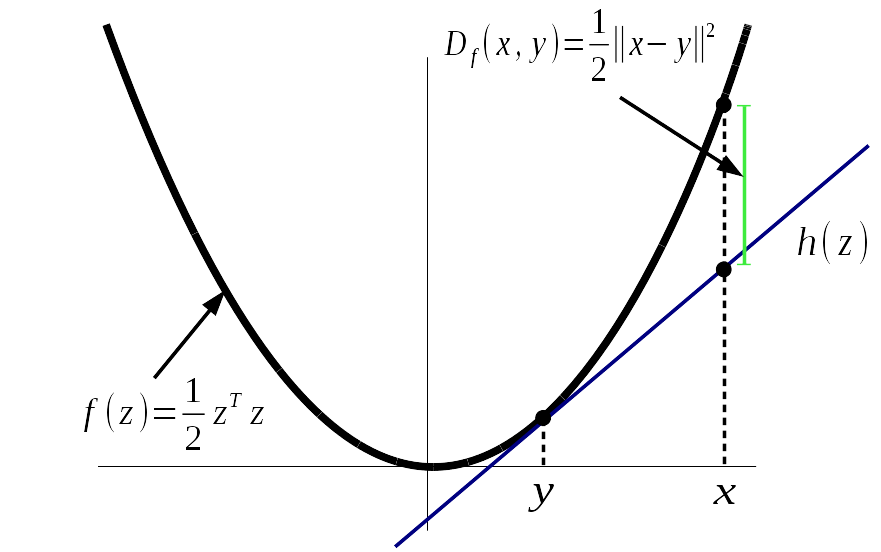
\includegraphics[width=0.6\columnwidth]{Figures/bregman_projection}
	\end{center}
	\caption{Geometry of the Bregman divergence with the seed function $f(z)=\frac{1}{2}z^\intercal z$. $h(z)$ is a hyperplane tangent to $f(z)$ at $y$. While it accurately represents $f(y)$, it underestimates $f(x)$. The Bregman divergence measures how much the representation of $f(x)$ on $h(z)$ \emph{diverges} from $f(x)$ (in green).}
	\label{fig:bregman-projection}
\end{figure}

The scalar divergence can be directly adapted to SPD matrices as:
\begin{equation}
\divB{f}(\P_1,\P_2) = \varphi(\P_1) - \varphi(\P_2) - \varphi'(\P_2)(\P_1 - \P_2) \ ,
\end{equation}
where the seed function $f$ is combined with a function $g: \GenMa \rightarrow \Re^\dc$ that maps an SPD matrix to a vector containing its eigenvalues: $\varphi = f \circ g$. 
$g$ can also be the trace function, $g: \GenMa \rightarrow \Re$ that maps an SPD matrix to its trace.
For convenience, $f \circ g$ will be referred to as $f(X)$ or $f(\P)$ for matrices. 

Depending on the seed function used, various divergences can be defined from the Bregman divergence. 
However, the mean induced by a Bregman divergence is independent of the seed function. 
It always correspond to the center of mass, i.e. the arithmetic mean \cite{nielsen_sided_2009}.
\\ \\ \textbf{Euclidean divergence} \\

A first Bregman divergence could be defined from the Frobenius norm~\cite{dhillon_matrix_2007}, with $f(x) = \frac{1}{2} \lVert x \rVert_F^2$:
\begin{equation}
\divB{E}(\P_1, \P_2) = \frac{1}{2}\lVert \P_1-\P_2 \rVert _F^2 \ .
\label{eq:div-eucl}
\end{equation}
In the Euclidean case, this divergence is equivalent to the square distance and consequently the mean of SPD matrices based on the Euclidean divergence corresponds to their arithmetic mean, see Eq.~\eqref{eq:mean_arithmetic}.
\\ \\ \textbf{Kullback-Leibler divergence} \\
Using the \emph{negative Shannon entropy} $f(x) = \sum_\nb x_\nb \log x_\nb$ yields the \emph{Kullback-Leibler} divergence~\cite{nielsen_sided_2009}.
It is also known as the \emph{relative entropy} or \emph{discrimination information}. 
The Kullback-Leibler divergence was introduced in information theory to measure the difference between two probability distributions over the same alphabet.
Given a set $\mathfrak{X} = \left\lbrace \x, \X, P \right\rbrace$, where:
\begin{itemize}
\item $\x \in \Re^{\dc}$ is a variable,
\item $\X \in \Re^{\dc \times \dt}$ is the set of all possible values of $\x$, \textit{i.e.} the \emph{alphabet}, and
\item $P$ is the probability distribution of $\x$ over $\X$ 
\end{itemize}
The Kullback-Leibler divergence measure the different between $P_1(\x)$ and $P_2(\x)$, both defined over $\X$:
\begin{equation}
\divB{KL}(P_1(\x), \P_2(\x)) = \sum_{i}^{\dt} P_1(\x_i) \log \frac{P_1(\x_i)}{P_2(\x_i)}
\label{eq:kl} 
\end{equation}
if both distribution are normal, 
\begin{equation}
P(\x) = \mathcal{N}(\mu, \P) = \frac{1}{(2\pi)^{\dc/2}\det(\P)^{1/2}} \left\lbrace \exp\left( -\frac{1}{2}(\x-\mu)^{T} \P^{-1}(\x-\mu) \right)  \right\rbrace
\label{eq:normal-distr}
\end{equation}
\eqref{eq:normal-distr} in \eqref{eq:kl},
\begin{equation}
\divB{KL}(P_1(\x), P_2(\x) = \frac{1}{2} \left( (\mu_1-\mu_2)^T \P_2^{-1}(\mu_1-\mu_2) - \log \det (\P_2^{-1}\P_1) + \tr(\P_2^{-1} \P_1) - \dc \right) \ .
\label{eq:div-kl-gen}
\end{equation}
When $P_1(\x)$ and $P_2(\x)$ are zero-centered, \eqref{eq:div-kl-gen} becomes:  
\begin{equation}
\divB{KL}(P_1(\x), P_2(\x) = \frac{1}{2} \left( \log \det (\P_1^{-1} \P_2) + \tr(\P_2^{-1} \P_1) - \dc \right) 
\label{eq:div-kl-proba}
\end{equation}
The Kullback-Leibler divergence correspond to the Bregman divergence of covariance matrices with the seed function $f(\P) = -\log \det (\P) $:
\begin{equation}
\divB{KL}(P_1(\x), P_2(\x) = \divB{KL}(\P_1, \P_2 = \frac{1}{2} \left( \log \det(\P_1^{-1} \P_2) + \tr(\P_2^{-1} \P_1) - \dc \right) \ .
\label{eq:div-kl}
\end{equation}
\\ \\ \textbf{S-divergence} \\
An example of a symmetric divergence is the S-divergence. 
It is obtained from the \emph{Jensen-Shannon} divergence which is a symmetrised Bregman divergence:
\begin{equation}
\begin{split}
\divB{J-S}(\P_1, \P_2) & = \frac{1}{2} \left( \divB{f}(\P_1,\frac{\P_1+\P_2}{2}) + \divB{f}(\frac{\P_1+\P_2}{2},\P_2) \right) 
\\
 & = \frac{1}{2} \left( \tr f(\P_1) + \tr f(\P_2) \right) - \tr f(\frac{\P_1+\P_2}{2}) \ .
\end{split} 
\label{eq:div-js}
\end{equation}
The S-divergence is obtained by using the logarithmic barrier function for the positive-definite cone $f(\P)=-\log \det(\P)$ as seen in $\divB{J-S}$, and the S-divergence between two SPD matrices corresponds to the Bhattacharyya divergence between them \cite{sra_positive_2016}:
\begin{equation}
\divB{S}(\P_1,\P_2) = \log \det(\frac{\P_1+\P_2}{2}) - \frac{1}{2}\log \det(\P_1 \P_2) \ .
\label{eq:div-s}
\end{equation}  
Despite its symmetry, S-divergence is not a metric: it does not satisfy the triangular inequality criterion. 
However, its squared root has been shown to be a distance~\cite{sra_positive_2016}.

Other symmetric divergences can be obtained in the same fashion; for instance, the \emph{Jeffreys divergence} which is a symmetrised Kullback-Leibler divergence: $\divB{J}(\P_1, \P_2) = \divB{KL}(\P_1, \P_2) + \divB{KL}(\P_2, \P_1)$~\cite{sra_positive_2016}.
\\ \\ \textbf{Log-det $\alpha$-divergence} \\
Another family of divergence is defined when the right- and left-sided divergences are mixed in a weighted manner.
One such family is the \emph{$\alpha$-divergence}~\cite{nielsen_clustering_2014}, and it is defined in this work by~\cite{chebbi_means_2012}:
\begin{equation}
\divB{f}^\alpha(\P_1,\P_2) = \frac{4}{1-\alpha^2}\left[ \frac{1-\alpha}{2} f(\P_1) + \frac{1+\alpha}{2}f(\P_2) - f \left( \frac{1-\alpha}{2}\P_1 + \frac{1+\alpha}{2}\P_2 \right) \right], \alpha^2 \neq 1
\label{eq:div-alpha}
\end{equation}
$\divB{f}^\alpha$ can be expressed in terms of Bregman divergence as:
\begin{equation}
\divB{f}^\alpha = \frac{4}{1-\alpha^2}\left[\frac{1-\alpha}{2}\divB{f}\left(\P_1, \frac{1-\alpha}{2}\P_1+\frac{1+\alpha}{2}\P_2\right) + \frac{1+\alpha}{2}\divB{f}\left(\P_2, \frac{1-\alpha}{2}\P_1 + \frac{1+\alpha}{2} \P_2 \right)\right], \alpha^2 \neq 1
\label{eq:div-alpha2}
\end{equation}
$\alpha$-divergences at $\alpha = \pm 1$ are obtained through the limit values $\lim_{\alpha \rightarrow \pm 1}\divB{f}^\alpha$. 
Using the logarithmic-barrier function yields:
\begin{equation}
\begin{split}
\divB{LD}^\alpha(\P_1,\P_2) &= \frac{4}{1-\alpha^2}\log \det \left(\frac{1-\alpha}{2}\left(\P_1 \P_2^{-1}\right)^{\frac{1+\alpha}{2}}+\frac{1+\alpha}{2}\left(\P_2 \P_1^{-1}\right)^{\frac{1-\alpha}{2}}\right), \quad -1 < \alpha < 1 \\
\divB{LD}^{1}(\P_1,\P_2) &= \tr \left( \P_2^{-1}\P_1-\eye \right) - \log \det \left(\P_2^{-1}\P_1 \right)\\
\divB{LD}^{-1}(\P_1,\P_2) &= \tr \left(\P_1^{-1}\P_2-\eye \right) - \log \det \left(\P_1^{-1}\P_2 \right) .
\end{split}
\label{eq:div-log-det-alpha}
\end{equation}   
$\divB{LD}^{1}$ and $\divB{LD}^{-1}$ are right- and left-sided Bregman divergences respectively.
At $\alpha=0$, the log-det $\alpha$ divergence yields a symmetric divergence corresponding to the Bhattacharyya divergence \cite{chebbi_means_2012,sra_positive_2016}. 
%%%%%%%%%%%%%%%%%%%%%%%%%%%%%%%%%%%%%%%%%%%%%%%%%%%%%%%%%%%%%%

All these distances and divergences are summed up in Table~\ref{tab:dist}.

\begin{table}[h]
  \centering
  \ra{1}
\begin{adjustbox}{center}
\resizebox{1.4\textwidth}{!}{
  \begin{tabular}{ l | c | c | c |}
    \cline{2-4}
    & Distance/Divergence & Mean & References \rule[-5pt]{0pt}{18pt} \\ \hline
    \multicolumn{1}{|l|}{Euclidean} & $\distF(\P_1, \P_2) = \lVert \P_1-\P_2 \rVert _F$ & $\PmE = \frac{1}{\Nb}\sum_{\nb=1}^{\Nb} \P_\nb$ & \rule[-5pt]{0pt}{18pt} \\  
    \multicolumn{1}{|l|}{Harmonic} & $\distH(\P_1, \P_2) = \lVert \P_1^{-1}-\P_2^{-1} \rVert _F$ & $\PmH = \left(   \frac{1}{\Nb}\sum_{\nb=1}^{\Nb} \P_\nb^{-1} \right)^{-1} $ & \cite{lim_matrix_2012} \rule[-5pt]{0pt}{18pt} \\ 
		 \multicolumn{1}{|l|}{Log-Euclidean} & $\distLE(\P_1, \P_2) = \lVert \log(\P_1)-\log(\P_2) \rVert_F$ & $\PmLE = \exp \left( \frac{1}{\Nb} \sum_{\nb=1}^{\Nb} \log(\P_\nb) \right) $ & \cite{arsigny_geometric_2007} 
		\rule[-5pt]{0pt}{18pt} \\    
     \multicolumn{1}{|l|}{Affine-invariant} & $\distAIRM(\P_1, \P_2) = \lVert \log(\P_1^{-1}\P_2) \rVert_F$ & Algorithm 3 in \cite{fletcher_principal_2004}  & \cite{moakher_differential_2005,fletcher_principal_2004} 
		\rule[-5pt]{0pt}{18pt} \\	
	\multicolumn{1}{|l|}{Kullback-Leibler} & $\divB{KL}(\P_1, \P_2) = \frac{1}{2} \left( \log \det(\P_1^{-1} \P_2) + \tr(\P_2^{-1} \P_1) - \dc \right) $ & $\PmKL = \frac{1}{\Nb}\sum_{\nb=1}^{\Nb} \P_\nb$ & \cite{chebbi_means_2012,kang_composite_2009} \rule[-5pt]{0pt}{18pt} \\
	\multicolumn{1}{|l|}{S-divergence} & $\divB{S}(\P_1,\P_2) = \log \det(\frac{\P_1+\P_2}{2}) - \frac{1}{2}\log \det(\P_1 \P_2)$ &  Eq. (17-20) in \cite{cherian_efficient_2011} & \cite{sra_positive_2016,cherian_efficient_2011} \rule[-5pt]{0pt}{18pt} \\
    \multicolumn{1}{|l|}{$\alpha$-divergence} & $\divB{LD}^\alpha (\P_1, \P_2)$ from Eq.~\eqref{eq:div-log-det-alpha} & Algorithm 1 in \cite{chebbi_means_2012} & \cite{chebbi_means_2012} \rule[-5pt]{0pt}{18pt} \\ 
    \multicolumn{1}{|l|}{Bhattacharyya} & $\divB{B}(\P_1, \P_2)=\left( \log \frac{ \det \frac{1}{2} (\P_1+\P_2)}{(\det (\P_1)\det(\P_2))^{1/2}} \right)^{1/2}$ & Algorithm 1 in \cite{chebbi_means_2012} & \cite{nielsen_matrix_2012,chebbi_means_2012} \rule[-5pt]{0pt}{18pt} \\ 
    \multicolumn{1}{|l|}{Wasserstein} & $\distW = \tr \left( \P_1 + \P_2 - 2 \left( \P_1^{1/2} \P_2 \P_1^{1/2} \right)^{1/2} \right)$ & Eq. 6.2 in \cite{agueh_barycenters_2011}  & \cite{agueh_barycenters_2011, barbaresco_geometric_2011} \rule[-5pt]{0pt}{18pt} \\ \hline
  \end{tabular}
  }
  \end{adjustbox}
  \caption{Distances, divergences and means considered in the experimental study.}
  \label{tab:dist}
\end{table}

\subsection{Minimum Distance to Mean Classifier for SSVEP}
\label{subsec:mdm}
The considered classifier is described in section \ref{subsec:fund_class}. 
It is given the name \emph{Minimum Distance to Mean} or MDM, and was inspired by~\citep{barachant_multiclass_2012} where it is limited to Riemannian mean.
%The considered classifier is referred to as Minimum Distance to Mean (MDM), and is inspired from~\cite{barachant_multiclass_2012} where it is limited to Riemannian mean. 
The covariance matrices of EEG trials are classified based on their distance to the centres of the classes (i.e. means or centroids).
To embed frequency information in the covariance matrices, we use a construction of matrices proposed in~\citep{congedo_new_2013}.
%In a SSVEP experiment with $\dF$ stimulus blinking at $\dF$ different frequencies, 
Let $\X \in \Re^{\dc\times\dt}$ be an EEG trial measured on $\dc$ channels and $\dt$ samples in an SSVEP experiment with $\dF$ stimulus blinking at different frequencies.  
The covariance matrices are estimated from a modified version of the input signal $\X$: 
\begin{equation}
	\X \in \Re^{\dc \times \dt} \rightarrow 	
	\begin{bmatrix}
		X_{\text{freq}_1}\\ \vdots \\ X_{\text{freq}_{\dF}} \\
	\end{bmatrix}
	\in \Re^{\dF\dc \times \dt} \ ,
	\label{eq:ext_data}
\end{equation}
where $X_{\text{freq}_\df}$ is the input signal $\X$ band-pass filtered around frequency $\text{freq}_\df$, $\df=1, \ldots, \dF$. 
Thus the resulting covariance matrix $\P$ belongs to $\mathcal{M}_{\dF\dc}$. 
Henceforth, all SSVEP EEG signals will be considered as filtered and modified by Eq.~\eqref{eq:ext_data}.

For ERP paradigm with a number $E$ of different ERPs, the modified signal is the concatenation of the original signal and the grand averages of trials containing the target ERPs $\bar{X}_e$, $e=1, \ldots, E$:
\begin{equation}
\X \in \Re^{\dc \times \dt} \rightarrow 	
\begin{bmatrix}
 \bar{X}_1\\ 
\vdots \\
\bar{X}_E \\
X\\
\end{bmatrix}
\in \Re^{(E+1)\dc \times \dt} \ ,
\label{eq:ext_data_erp}
\end{equation}
The resulting covariance matrix will be of size $((E+1) \times \dc)^2$. 
%Adding a non-target class, it is a multiclass classification with $\dK=E+1$ classes.

For SSVEP classification, $\dK = \dF + 1$ classes are considered: one class for each target frequency, and one for the resting state.
As described in Algorithm~\ref{alg:mdm}, from $\dT$ labelled training trials $ \left\{ \X_{\ti} \right\}_{\ti=1}^{\dT}$ recorded per subject, $\dK$ centres of classes $\Pm^{(\ci)}$ are estimated (step~\ref{op:class_center}). 
In this step, outliers matrices are removed to have a reliable mean estimation \citep{barachant_riemannian_2013}.
A new unlabelled test trial $\Y$ is predicted to belong to the class whose mean $\Pm^{(\ci)}$ is the closest to the trial covariance matrix, w.r.t. one of the distances from Table~\ref{tab:dist} (step~\ref{op:decision}).

\begin{algorithm}
\caption{Minimum Distance to Mean Classifier}
\label{alg:mdm}
	Inputs: $\X_{\ti} \in \Re^{\dF \dc\times\dt}$, for $\ti = 1, \ldots, \dT$, a set of labelled EEG trials. \\
	Inputs: $\setindex(\ci)$, a set of indices of trials belonging to class $\ci$. \\
	Input: $\Y \in \Re^{\dF \dc\times\dt}$, an unlabelled test EEG trial. \\
	Output: $\clout$, the predicted label of $\Y$.
	\begin{algorithmic}[1]
	\State Compute covariance matrices $\P_{\ti}$ of $\X_\ti$ 
	\State \textbf{for} $\ci$ = 1 \textbf{to} $\dK$ \textbf{do}
	\State \quad Compute centre of class : $\Pm^{(\ci)}=\Rm(\P_{\ti}:\ti \in \setindex(\ci))$
	\label{op:class_center}
	\State \textbf{end}
	\State Compute covariance matrix $\P$ of $\Y$, and classify it : $\clout = \arg \min_{\ci} \dist(\P, \Pm^{(\ci)})$
	\label{op:decision}
	\State \textbf{return} $\clout$
	\end{algorithmic}
\end{algorithm}

where $X_{\text{freq}_\df}$ is the input signal $\X$ band-pass filtered around frequency $\text{freq}_\df$, $\df=1, \ldots, \dF$. 

From $\dT$ labelled training trials $ \left\{ \X_{\ti} \right\}_{\ti=1}^{\dT}$ recorded per subject, $\dK$ centres of class $\P_{\Rm}^{(\ci)}$ are estimated using Algorithm~\ref{alg:r_mean}. 
%The MDRM is then used for classification, as shown in Algorithm~\ref{alg:mdrm}. 
When an unlabelled test trial $\Y$ is given, it is classified as belonging to the class whose centre $\P_{\Rm}^{(\ci)}$ is the closest to the trial's covariance matrix (Algorithm~\ref{alg:mdm}, step \ref{op:decision}).
   
\begin{algorithm}
\caption{Offline Estimation of Riemannian Centres of Classes}
\label{alg:r_mean}
	Inputs: $\X_{\ti} \in \Re^{\dF \dc\times\dt}$, for $\ti = 1, \ldots, \dT$, a set of labelled trials. \\
	Inputs: $\setindex(\ci)$, a set of indices of trials belonging to class $\ci$. \\
	Output: $\P_{\Rm}^{(\ci)}$, $\ci = 1, \ldots, \dK$, centres of classes.
	\begin{algorithmic}[1]
	\State Compute covariance matrices $\cov{\textit{\ti}}$ of $\X_\ti$ %, Eq.~\eqref{eq:shrink}
	\label{op:cov_i}
	\State \textbf{for} $\ci$ = 1 \textbf{to} $\dK$ \textbf{do}
	\State \quad $\P_{\Rm}^{(\ci)}=\Rm(\cov{\textit{\ti}}:\ti \in \setindex(\ci))$ , Eq.~\eqref{eq:mean}
	\label{op:class_center}
	\State \textbf{end}
	\State \textbf{return} $\P_{\Rm}^{(\ci)}$ 
	\end{algorithmic}
\end{algorithm}

\section{Online Classification}
\label{sec:online-classification}

\subsection{Curve-Based Online Classification} %pas Gradient-based 

\begin{algorithm}
\caption{Curve-based Online Classification}
\label{alg:online}
	Inputs: hyper-parameters $\ws$, $\deltaN$, $\dd$, and $\pthres$.\\
	Inputs: $\P_{\Rm}^{(\ci)}$, $\ci = 1, \ldots, \dK$, centres of classes from Algorithm~\ref{alg:r_mean} (offline training). \\
	Inputs: Online EEG recording $\onlineX(\si)$. \\
	Output: $\cloutOn(\si)$, online predicted class.
	\begin{algorithmic}[1]
	\State $\di=1$
	\State \textbf{for} $\si = \ws$ \textbf{to} $\dr$ \textbf{step} $\deltaN$
	\State \quad Epoch $\Xs{\di}$, Eq.~(\ref{eq:online_epoch}), and classify it with Algorithm~\ref{alg:mdm}
	\label{op3:epoch_and_classify}
	\State \quad \textbf{if} $\di \geq \dd$ %$\si \geq \ws+(\dd-1)\deltaN$
	\label{op3:test_len}
	\State \quad \quad Find the most recurrent class in $\clarray = \clout_{\tj \in \Dindex(d)}$:
	$\cloutmp = \argmax_{\ci} \pocc(\ci)$, Eq.~\eqref{eq:occ_prob}
	\label{op3:get_rho}
	\State \quad \quad \textbf{if} $\pocc(\cloutmp)>\pthres$
	\label{op3:test_rho}
	\State \quad \quad \quad Compute $\disvec_{\cloutmp}$, Eq.~\eqref{eq:dist_vec} %This line can be left out
	\label{op3:get_disvec}
	\State \quad \quad \quad \textbf{if} $\disvec_{\cloutmp} < 0$ 
	\label{op3:test_disvec}
	\State \quad \quad \quad \quad \textbf{return} $\cloutOn = \cloutmp$
	\label{op3:valid_class}
	\State \quad \quad \quad \textbf{end}
	\State \quad \quad \textbf{end}
	\State \quad \textbf{end}
	\State \quad $\di = \di+1$
	\label{op3:increment_d}
	\State \textbf{end}
	\end{algorithmic}
\end{algorithm}

%Sylvain: Est ce qu'on peut donner une formule pour calculer \pocc qui soit pas trop ridicule ? 
%Emmanuel: Comme \pocc est une probabilite, sa formule serait (tu peux uncomment pour voir ce que ca donne: 
%\[
%\pocc(j) = \frac{\textrm{number of outcome }j}{\textrm{total number of outcomes}}
%\]
%qui pourait s'ecrire aussi:
%\[
%\pocc(j) = \frac{1}{D}| \{ i \in \{ 1, \dots, \dd \}:\clout_i = j \} |
%\]
%ou peut etre tout simplement:
%\[
%\pocc(j) = \frac{1}{D} \sum_{i=1}^{\dd} \left[\clout_i = j \right]
%\]
%Sylvain: changer les parametres et dire qu'on prend les centers de classe.
%Emmanuel: C'est fait! 


In offline synchronous BCI paradigm, cue onset is used as reference for the localisation of a brain response, e.g. an evoked potential. 
Nonetheless most of the BCI applications are online and asynchronous; cue onsets are not known, thus designing online version of BCI algorithms %, even well documented ones, 
is not a trivial task. 
%In online and asynchronous experiment, there is no such cue onset and the adaptation of the algorithm for online processing is not trivial and often difficult.
The approach introduced here identifies a period (\textit{i.e.} time interval) in the online EEG $\onlineX \in \Re^{\dF\dc\times\dr}$, where $\dr$ is the number of recorded samples, associated with a high probability (above the threshold) of observing an SSVEP at a specific frequency, as illustrated in Algorithm~\ref{alg:online}. % (i.e. beyond a predefined threshold). 
  
To locate this interval, we focus on the last $\dd$ recorded EEG overlapping epochs 
%$ \left\{ \Xs{\ensuremath{i}} \in \Re^{\dF\dc \times \ws} \right\}_{\tj \in \Dindex(d)} $, 
$ \left\{ \Xs{\tj} \in \Re^{\dF\dc \times \ws} \right\}_{\tj \in \Dindex(d)} $,
with the set of indices $\Dindex(d) = \di-\dd +1,\ldots,\di-1,\di$; 
where $\di$ is the index of the current epoch $\Xs{\di}$ in the online recording $\onlineX(n)$. 
Epochs have size $\ws$, and the interval between two consecutive epochs is $\deltaN$, with $\ws > \deltaN $:
%Epochs $\Xs{\di}$ are obtained by sliding a window of size $\ws$ by a step of size $\deltaN$ every time $\deltaN$ new samples are available (step~\ref{op3:epoch}):
%\[ \Xs{\di} = \onlineX(\time) \Big|_{\time=\si-\ws,\ldots,\si} \]
\begin{equation}
\label{eq:online_epoch}
 \Xs{\di} = \onlineX(\si-\ws,\ldots,\si) \ .
\end{equation}
%Consecutive $\Xs{\di}$ overlap, with $\ws > \deltaN $.
%To sum up, $\Xs{\di}$ slides over all the signal to give successive epochs for the online framework.
To obtain the first $\dd$ epochs $\Xs{\ensuremath{\tj \in \Dindex(d)}}$, at least $\ws+(\dd-1)\,\deltaN$ samples of $\onlineX$ should be recorded (step~\ref{op3:test_len}).

The classification outputs $\clout_{\tj \in \Dindex(d)}$ obtained in step~\ref{op3:epoch_and_classify} by applying Algorithm~\ref{alg:mdm} on $\Xs{\ensuremath{\tj \in \Dindex(d)}}$ are stored in a vector $\clarray$, 
which always contains the latest $\dd$ classification outputs.
The class that occurs the most in $\clarray$ (step~\ref{op3:get_rho}), with an occurrence probability $\pocc(\ci)$ above a defined threshold $\pthres$, 
%(where $\pocc$ is a vector of size $\dF$ containing the probabilities of occurrence of each class in $\clarray$)
is considered to be the class, denoted $\cloutmp$, of the ongoing EEG recording $\onlineX(\si)$. 
The vector $\pocc$ is defined as:
% \begin{equation}
% \label{eq:occ_prob}
% \begin{split}
%   \pocc(\ci) = \frac{\#\{ \clout_{\tj \in \Dindex(d)} = \ci \}}{\dd} & , \text{ for } \ci = 1, \ldots, \dK, \\
%   \text{and} \ \ \ \ \ \ \ \ \ \ \ \ \ \ \ \ \cloutmp = {\argmax}_{\ci} & \ \pocc(\ci) \ .
% \end{split}
% \end{equation}
\begin{equation}
\label{eq:occ_prob}
  \pocc(\ci) = \frac{\#\{ \clout_{\tj \in \Dindex(d)} = \ci \}}{\dd}, \text{ for } \ci = 1, \ldots, \dK,
\end{equation}
with $\cloutmp = {\argmax}_{\ci} \ \pocc(\ci)$; % and \revise{$\pocc(\cloutmp) > \pthres$}.
then $\pocc(\cloutmp)$ is compared to the threshold $\pthres$.
If $\pthres$ is not reached within the last $\dd$ epochs, the classification output is held back, and the sliding process continues until $\pthres$ it is reached. 
%and with a new epoch $\Xs{\di+1}$ classified, and $\clarray$ updated with $\clout_{\di+1}$. 
%The process carries on until $\pthres$ is reached.    
In the last $\dd$ epochs, once a class $\cloutmp$ has been identified,  a curve direction criterion is introduced to enforce the robustness of the result.  
For class $\cloutmp$ to be validated, this criterion requires that the direction taken by the displacement of covariance matrices $\cov{\textit{\tj} \in \Dindex(\textit{\di})}$ be toward the centre of class $\P_{\Rm}^{(\cloutmp)}$. %\classM{l}
Hence $\disvec_{\cloutmp}$, the sum of gradients (\textit{i.e.} differentials) of the curve made by distances from $\cov{ \textit{\tj} \in \Dindex(\textit{\di})}$ to $\P_{\Rm}^{(\cloutmp)}$ should be negative (step~\ref{op3:test_disvec}):
%%A window of size $w_s$ seconds is slided from $t = t_0 - w_s$ to $t_0$ with a step of $\Delta t$ seconds.
%%The most represented class in the $\dd$ last classifications, with an occurrence probability $\pocc(j)$ reaching a predetermined threshold $\pthres$, is considered to be the class of the current EEG samples.  
%%%Sylvain : inclure une ref a l'algo avec la ligne
%%If $\pthres$ is not reached within $\dd$ epochs, no classification is done and the sliding window process goes on. 
%%When considering $\dd$ epochs, if a specific class is selected several times in a row,  a curve direction criterion is introduced to enforce the stability of the results. %validate the output. %gradient
%Once the classification result is more or less \emph{steady} on a specific class, a direction criterion is introduced to validate the output. %gradient
%Sylvain : idem, ref a la ligne dans l'algo
\begin{equation}
\label{eq:dist_vec}
\begin{split}
  \disvec_{\cloutmp} &= \sum_{\tj \in \Dindex(\di)} \frac{\Delta \diffdist_{\cloutmp}(\tj)}{\Delta \tj} 
  \ = \sum_{\tj=\di-\dd+2}^{\di} \diffdist_{\cloutmp}(\tj) - \diffdist_{\cloutmp}(\tj-1)
	\ < 0 
	\\
  & \text{with} \ \ \ \ \diffdist_{\cloutmp}(\tj) = \frac{\distR (\cov{\textit{\tj}}, \P_{\Rm}^{(\cloutmp)} )}{\sum_{\ci=1}^{\dK} \distR (\cov{\textit{\tj}},\P_{\Rm}^{(\ci)})} \ .
\end{split}
\end{equation}
%$L$ is the number of classes, and $d_R(\cdot,\cdot)$ is the Riemannian distance between two covariance matrices at $\Delta_t = n$.\\  

The occurrence criterion is inspired by the dynamic stopping of \citep{verschore_dynamic_2012}; there is no fixed trial length for classification.
The occurrence criterion ensures that the detected user intention is unaffected by any short time disturbances due to noise or subject inattention, as presented in Algorithm~\ref{alg:online}. 
This approach offers a good compromise to obtain robust results within a short and flexible time.

The curve direction criterion solves both the problems of latency in the EEG synchronisation and of the delays inserted by the EEG epochs processing. 
Indeed, some EEG epochs gather signals from different classes and might be wrongfully classified if the decision is solely based on the distance with the centre of the class.
% a given epoch may be wrongly assigned to a class previous EEG states might 
%This might results in previous EEG states being detected as current states while the user has intentionally moved to another state. 
This situation and the effect of the curve direction criterion are well shown in Section~\ref{sec:ssvep_response_delay}. 
Ensuring that the covariance matrices are displaced toward the centre of the detected class provides a guaranty that it matches with the current EEG state.
%Having the displacement of covariance matrices toward the center of the detected class guarantees that it matches the current EEG state (user's target).
Inversely, if the direction of the curve is moving away from the centre of the detected class, it might indicate that there have been a change in the EEG state that has not been detected.

The Algorithm~\ref{alg:online} has four hyperparameters: $\ws$, $\deltaN$, $\dd$, and $\pthres$.
The values of $\ws$, $\dd$, and $\pthres$ are set through cross validation and are given in Section~\ref{sec:ssvep_response_delay}.
Although a large window size $\ws$ is expected to increase the classification accuracy, it increases the response time, thus reducing the time resolution, and extends the overlap between different EEG states.
The step size $\deltaN$ should be set to a minimum value to allow a maximum number of overlapping epochs ($\dd$) within a short time. 
However, it should be large enough to avoid too many calculations within a time interval with small or inexistent changes in EEG states.
% However, it should be large enough to yield the difference between two consecutive epochs. 
% A large enough step size will also avoid too many calculations within a time interval with no change in EEG states.  
If the number of the epoch  $\dd$ is too small, the classification will be sensitive to non-intentional and abrupt changes in the EEG.
A too large $\dd$ will increase the momentum and reinforce the influence of the past EEG signals.
% make the classification depends too much on past EEG epochs. 
It should also be mentioned that both the occurrence and the curve direction criteria cannot have a significant impact if the value of $\dd$ is too small.
The probability threshold parameter $\pthres$ acts like a rejection parameter: high $\pthres$ values correspond to high rejection rate. 
%The optimal value is determined through cross validation.  
%- Having D epoch constitute a memory and gives a trend in the measurement    

\subsection{Outliers Removal with Riemannian Potato}
\label{sec:potato} 
Outliers in the training data might affect the Riemannian mean of classes in the MDRM classification scheme.
To alleviate this effect, an approach called the Riemannian potato, introduced in \citep{barachant_riemannian_2013}, is exploited.
In this approach, all trials are represented by their covariance matrices $\P_i$.
A reference covariance matrix is estimated, e.g. Riemannian mean of all trials $\P_{\mu}$.
The Riemannian distances $\distR_i$ between each $\P_i$ and $\P_{\mu}$ are computed. 
Any trial that lies too far, \textit{i.e.} beyond a certain threshold, from the reference matrix $\P_{\mu}$ in terms of Riemannian distance is rejected.
In \citep{barachant_riemannian_2013}, the distance z-score thresholding is defined as:
\begin{equation}
	\zs(\distR_i) = \frac{\distR_i - \mu}{\sigma} > \zs_{th}
\label{eq:potato}
\end{equation}
where $\mu$ and $\sigma$ are respectively the mean and standard deviation of distances $\left\{ \delta_i \right\}_{i=1}^I$. 
%Eq.~\eqref{eq:potato} defines the Riemannian potato. 
In other words, any trial $\P_i$ whose z-score $\zs(\distR_i)$ is larger than the threshold $\zs_{th}=2.5$ is rejected.

In this work, we propose a slightly different application of the Riemannian potato where the outliers are removed per class. 
Hence for $K$ class, $K$ Riemannian potatoes are defined $\left\{ \P^k_{\mu}, \mu^k, \sigma^k \right\}_{k=1}^K$.
Since Riemannian distances to geometric mean do not have a Gaussian distribution, we make use of the geometric mean for $\mu$, the geometric standard deviation for $\sigma$ and the geometric z-score.
They are defined as follows \citep{congedo2013eeg}:
\begin{equation}
  \begin{split}
    \mu^k = & \exp \left( \frac{1}{I} \sum_i \ln(\distR^k_i) \right)\\
    \sigma^k = & \exp \left( \sqrt{\frac{1}{I} \sum_i \left( \ln \left( \distR^k_i / \mu^k \right) \right)^2 } \right)\\
    \zs(\distR^k_i) = & \frac{\ln \left( \distR^k_i / \mu^k \right)}{\ln(\sigma^k)} \ .\\
  \end{split}
\end{equation}
Through cross-validation, the z-score threshold is set to $\zs_{th}=2.2$.
Moreover, outliers are removed iteratively. 
Each time outliers are rejected, a new centre of class is computed and used as reference for the next iteration.
The iterations continue until convergence, \textit{i.e.} no more outlier
found. 
\section{Experimental Validation}
\label{sec:experimental-validation}

\subsection{Covariance Estimators Comparison}

\begin{figure}[ht!]
  \centering
  \pgfimage[width=1.0\columnwidth]{Figures/accuracy_errorbar-eps-converted-to.pdf}
  %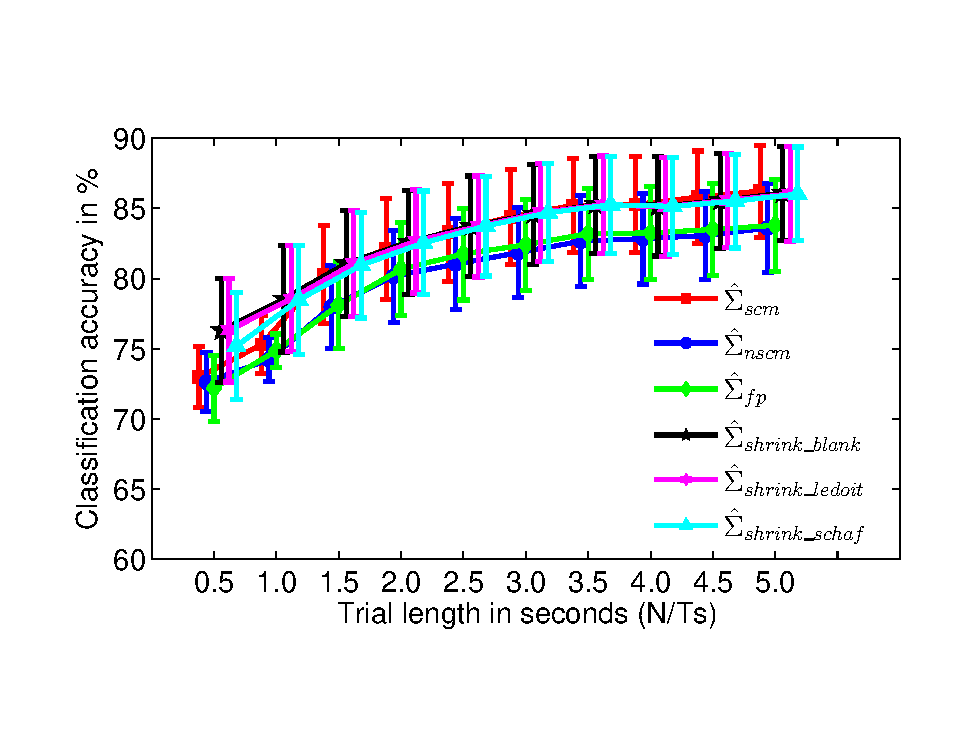
\includegraphics[width=1.0\columnwidth]{Figures/accuracy_errorbar.eps}  
  \caption{Comparison of covariance estimators in terms of classification accuracy
    obtained with MDRM with increasing EEG trial length. For each trial length, the average accuracy 
    across all subjects and across all replication is shown. 
    Bars indicate the error of the mean, i.e. standard deviation divided by the square root of $n-1$, $n$ = number of samples.}
    \label{fig:acc_errorbar}
  \end{figure}

%To perform classification on the Riemannian manifold, it is crucial to ensure that the covariance matrices obtained from the measured signal are symmetric positive-definite, that they are well conditioned and representative of the samples. 
In this section, the effectiveness of covariance matrix estimators is evaluated for SSVEP signals. 
The evaluation is done in terms of classification accuracy
%, information transfer rate (ITR),
 and integrated discrimination improvement (IDI), obtained by each estimator (see Section~\ref{sec:covmat-estimation}) with respect to the SCM estimator while using the offline MDRM classifier. 
%\textcolor{red}{QB:Si c est MDRM, toutes les comparaisons sont effectu\'ees  sur algo offline, et non online. ce qui est incoherent avec le fait de decouper des epoch (on parle de epoch size)... Idem legende Fig 1!}. 
The different conditioning of covariance matrices are also investigated.
%The estimators analyzed are described in. 

%\subsubsection{Methods}
A bootstrapping with 1000 replications is performed to assess the performances of each estimator. 
%From the pool of recorded samples available for each subject, a set of training data is randomly sampled with replacement; similarly, a set of test data is selected, with no overlap between the two sets. Class-mean matrices are obtained from the training set, and the classification performed on the test set. This is done for each matrix estimator (used to compute covariance matrix of samples), and the performance of each estimator are calculated. And the process is repeated 1000 times.
Estimators are compared on 10 trial lengths $t \in \{ 0.5, 1.0, \dots 5.0\}$ seconds, as these are known to affect the estimators performance. Here $\dt \in \{ 128, 256, \dots, 1280 \}$ is computed as $\dt=t \times T_s$.

Figure~\ref{fig:acc_errorbar} shows the classification accuracy of each estimator. 
The increase in the accuracy can be attributed to the fact that the relevant patterns in EEG accumulate with the trial length, producing better estimation of the covariance matrices. 
%It is as well due to the fact that an increase in sample size results in a
This is known to be particularly true for the SCM estimator and it could be seen in Figure~\ref{fig:acc_errorbar}.
It appears that shrinkage estimators (especially Ledoit and Sch\"afer) are less affected by the reduction of epoch sizes than the other estimators. This is a direct consequence of the regularisation between the sample covariance matrices and the targeted (expected) covariance matrix of independent variables.  
%The information of Figure~\ref{fig:acc_errorbar} are congruent with those of Figure~\ref{fig:itr_errorbar}; ITR increases as the trial length decreases. The transfer rate is higher for shrinkage estimators with shorter epoch sizes, while maintaining correct accuracy.

For computational purposes, it is important to look at the matrix conditioning. 
Figure~\ref{fig:eigenvalue_range} shows the ratio $\mathcal{C}$ between the largest and smallest eigenvalues: in well-conditioned matrices, $\mathcal{C}$ is small. 
Shrinkage estimators offer better conditioned matrices whereas the SCM, NSCM, and Fixed Point matrices are ill-conditioned below two seconds of trial length, and may result in singular matrices. 

%\begin{figure}[htb!]
%  \centering
%  %1CL \begin{minipage}[b]{0.62\linewidth}
%  \begin{minipage}[b]{0.95\linewidth}
%    \pgfimage[width=1\textwidth]{Figures/eigenvalue_range-eps-converted-to.pdf}
%    % 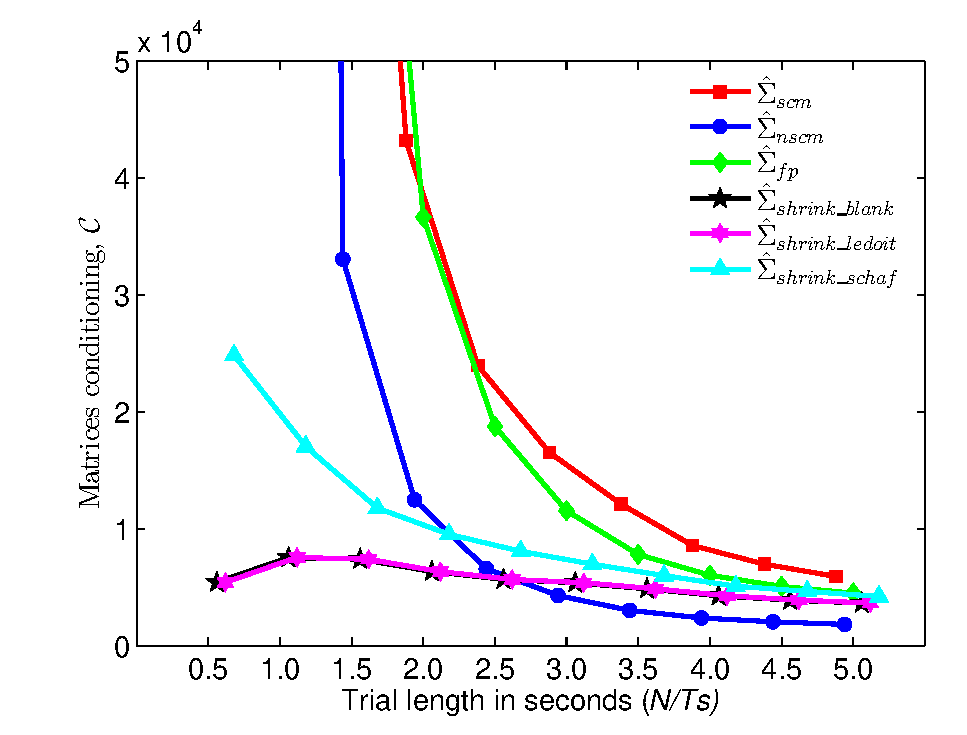
\includegraphics[width=1\textwidth]{Figures/eigenvalue_range.eps}
%    %\subcaption{}
%    \label{fig:eigenvalue_range}
%  \end{minipage}
%        
%  %1CL \begin{minipage}[b]{0.62\linewidth}
%  \begin{minipage}[b]{0.95\linewidth}
%    \pgfimage[width=1\textwidth]{Figures/idi-eps-converted-to.pdf}
%    % 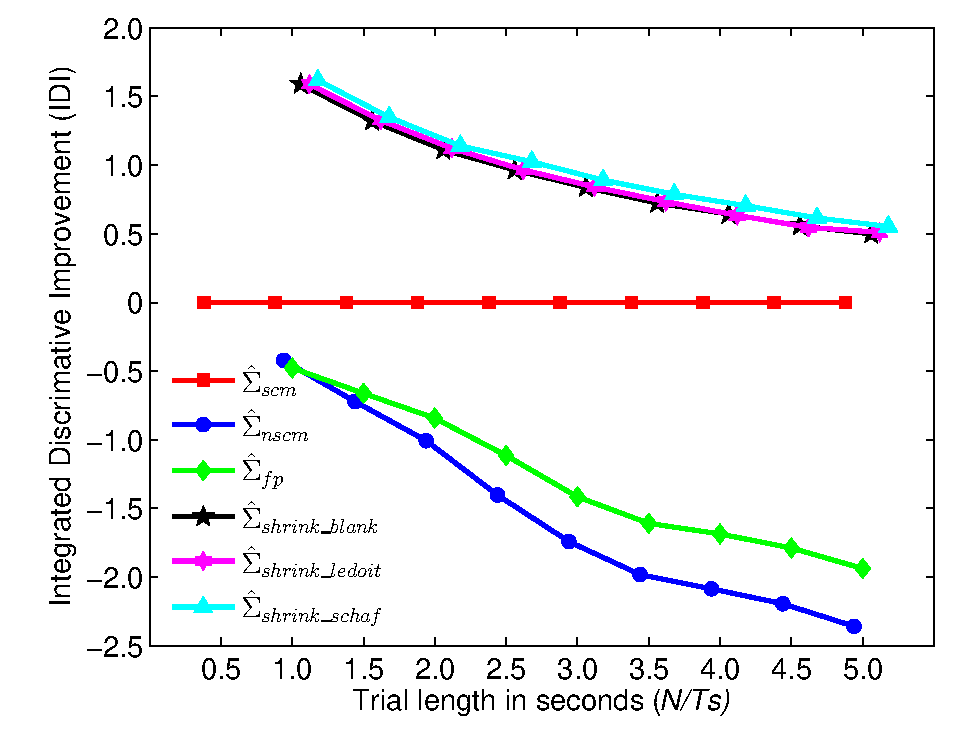
\includegraphics[width=1\textwidth]{Figures/idi.eps}
%    %\subcaption{}
%    \label{fig:idi}
%  \end{minipage}
%        
%        \caption{(a) Covariance matrices condition expressed as the ratio $\mathcal{C}$ between largest and smallest eigenvalues for the different covariance estimators. The comparison is done for increasing EEG trial length. (b) Integrated discrimination improvement brought to the classification task by various estimators along varying trail length. The indicated IDI values are multiplied by $10^{2}$. $\cov{scm}$ is used as baseline. }
%        \label{fig:class_idi}
%\end{figure}


\begin{figure}[htb!]
\centering
\subfigure[]{
\pgfimage[width=0.6\textwidth]{Figures/eigenvalue_range-eps-converted-to.pdf}
\label{fig:eigenvalue_range}
}
\subfigure[]{
\pgfimage[width=0.6\textwidth]{Figures/idi-eps-converted-to.pdf}
\label{fig:idi}
}
%\subfigure[]{
%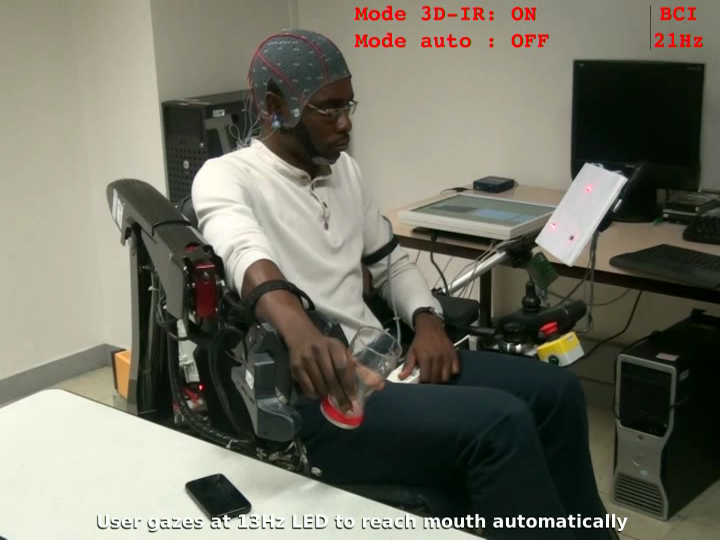
\includegraphics[width=0.45\textwidth]{Figures/esta03}
%\label{fig:esta03}
%}
\caption{(a) Covariance matrices condition expressed as the ratio $\mathcal{C}$ between largest and smallest eigenvalues for the different covariance estimators. The comparison is made for increasing EEG trial length. (b) Integrated discrimination improvement brought to the classification task by various estimators along varying trail length. The indicated IDI values are multiplied by $10^{2}$. $\cov{scm}$ is used as a baseline. } 
\label{fig:class_idi}
\end{figure} 



On Figure~\ref{fig:idi}, the Integrated Discrimination Improvement (IDI), as defined in \cite{pencina_evaluating_2008}, is computed for the different estimators and trial lengths. 
The SCM is used as a reference for improvement, as this is the most popular estimator in the literature. 
Negative IDI means a deterioration in the method discrimination ability. 
It is clear that shrinkage estimators increase the discrimination power of the classifier. 
However, despite being more complex than the SCM, the NSCM and the Fixed Point estimators decrease the discrimination ability of classifiers.     
From Figures~\ref{fig:acc_errorbar} and~\ref{fig:idi}, it is apparent that the difference in performance between the SCM and shrinkage estimators reduces as the trial length increases.
The simplicity of the SCM plays a favourable role: it is an attractive method for longer trials. 
%However for trial lengths compatible with a reasonable ITR for man-machine interaction ($< 2$ sec), the shrinkage estimators offer better performances, with the Schafer estimator being the best. 
The $p$-values under the hypothesis that there is no improvement (\textit{i.e.} IDI = 0) from one estimator to another are all inferior to $10^{-47}$, ($p<10^{-3}$ indicating a statistically significant discriminatory improvement); hence the improvement is significant.
It should be noted that the estimation of covariance matrices is a trade-off between the quality of the estimate and the computation time required; this should be considered for real time processing.
    
\subsection{Effect of Outliers on Centre Estimation}

Outliers can affect the offline training of the $\dK$ centres of class $\P_{\Rm}^{(\ci)}$ by Algorithm~\ref{alg:r_mean}, which is crucial for the evaluation phase and online application.
Figure~\ref{fig:tan_plan_s16&17} shows representations of training covariance matrices $\P_{\ti}$ in the tangent space ($\S_{\ti}$), projected at the mean of all training trials, for the subjects with the lowest (\ref{fig:tan_plan_s16_a} and \ref{fig:tan_plan_s16_b}) and the highest (\ref{fig:tan_plan_s17_a} and \ref{fig:tan_plan_s17_b}) BCI performance. 
To obtain this visualisation, the first two principal components of a PCA applied on $\left\{ \S_{\ti} \right\}_{\ti=1}^{\dT}$ are selected.
In Figures~\ref{fig:tan_plan_s16_b} and~\ref{fig:tan_plan_s17_b}, the Riemannian potato presented in Section \ref{sec:potato} is applied; outliers in each class are removed.
%Riemannian potato only removes highly corrupted signals, allowing to remove outlier trials that negatively impact the estimation of class centers.
The interest of using a Riemannian potato is well seen in Figure \ref{fig:tan_plan_s16_a} and \ref{fig:tan_plan_s16_b}. 
In \ref{fig:tan_plan_s16_a}, the outliers are so distant from the rest of the class matrices that the centre of class is stretched away.
Applying a Riemannian potato removes the outliers, and the centre of class is better estimated (\ref{fig:tan_plan_s16_b}).

When training trials are not noisy, their covariance matrices are compact around their Riemannian mean. 
In this case the removal of outliers by the Riemannian potato does not influence, at least not significantly, the Riemannian mean. 
This is the case in Figure \ref{fig:tan_plan_s17_a} and \ref{fig:tan_plan_s17_b}.
Thus, applying the Riemannian potato is crucial for noisy data and will have a limited effect on clean data.
The impact of the Riemannian potato on the classification accuracy is discussed in Section \ref{sec:ssvep_response_delay}. 

\begin{figure}[hb!]
%\centering
\begin{adjustbox}{center}
\resizebox{1.2\textwidth}{!}{
\subfigure[]{
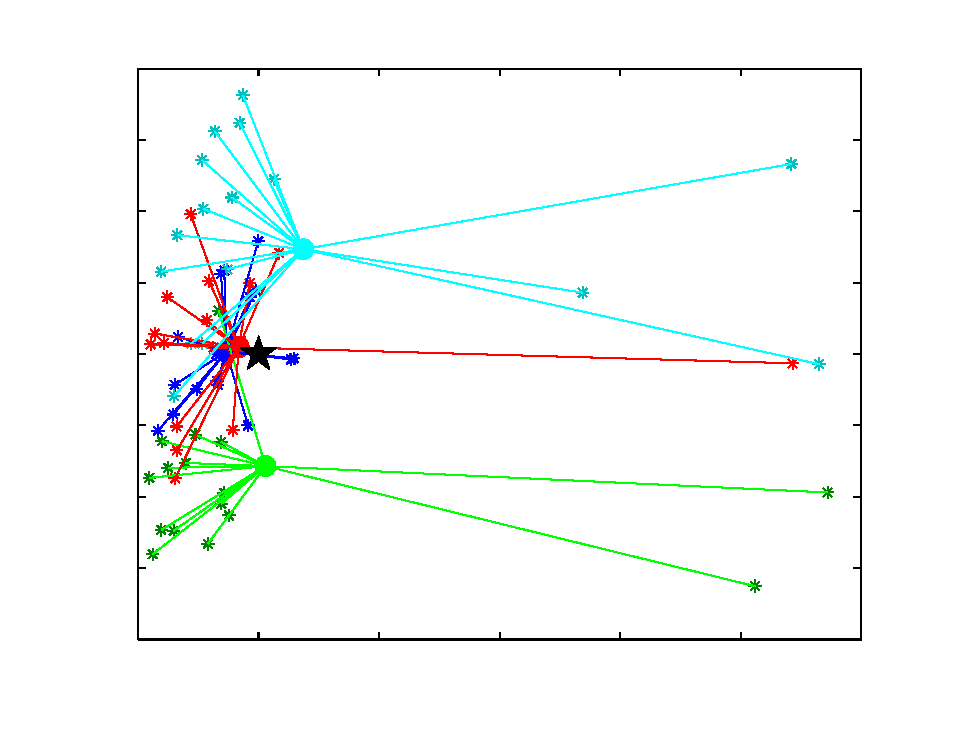
\includegraphics[width=0.6\textwidth]{Figures/tan_plan_2D_s16_b.eps}
\label{fig:tan_plan_s16_a}
}
\subfigure[]{
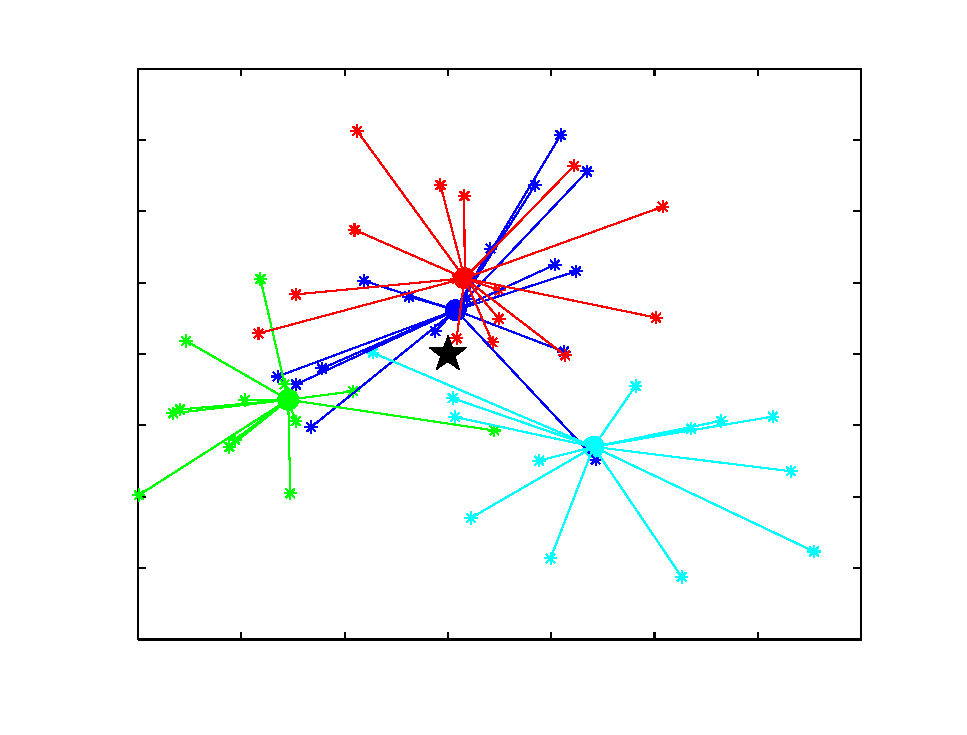
\includegraphics[width=0.6\textwidth]{Figures/tan_plan_2D_s16_a.eps}
\label{fig:tan_plan_s16_b}
}
}
\end{adjustbox}

\begin{adjustbox}{center}
\resizebox{1.2\textwidth}{!}{
\subfigure[]{
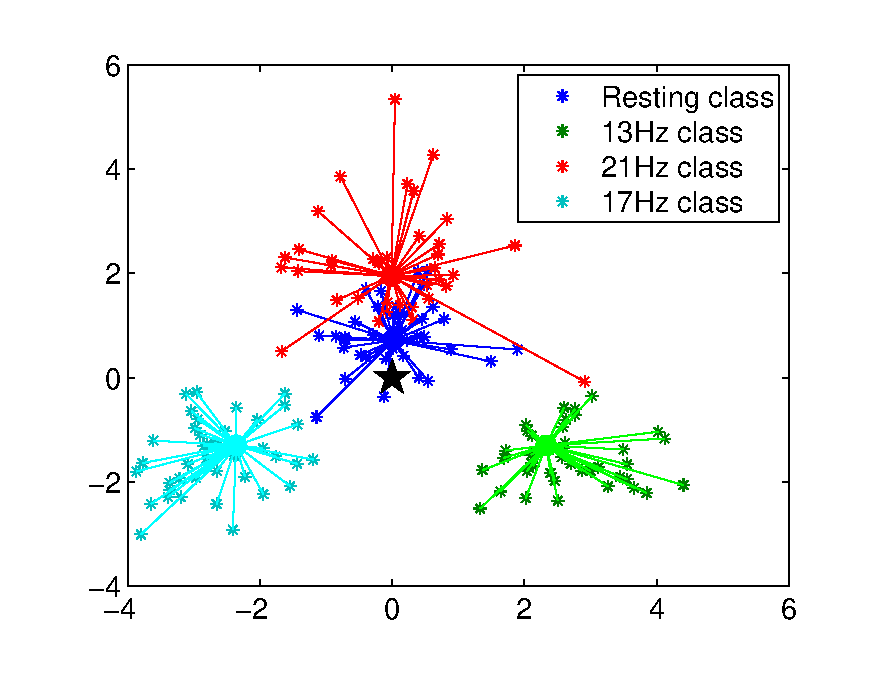
\includegraphics[width=0.6\textwidth]{Figures/tan_plan_2D_s17_a.eps}
\label{fig:tan_plan_s17_a}
}
\subfigure[]{
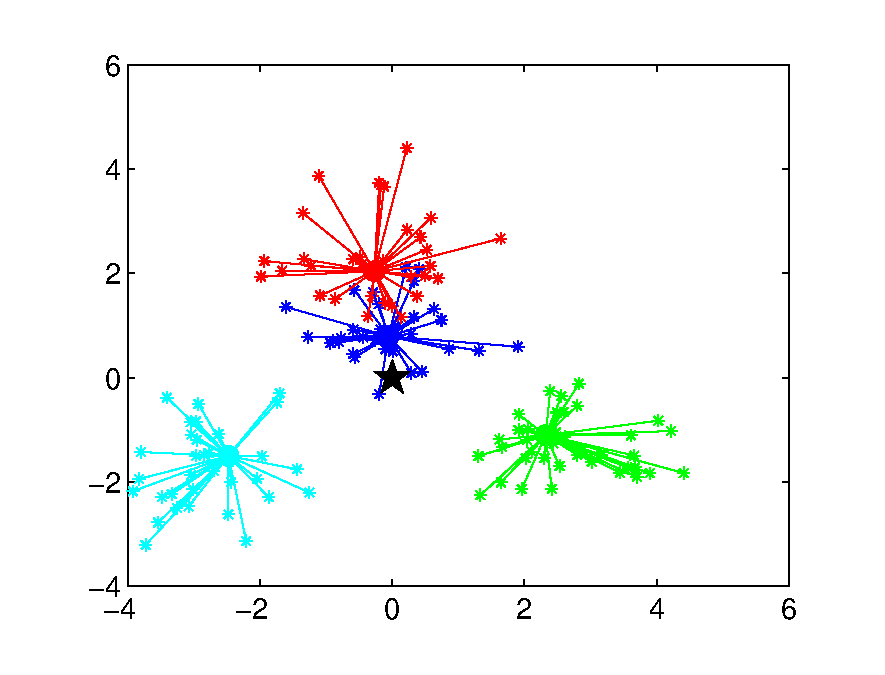
\includegraphics[width=0.6\textwidth]{Figures/tan_plan_2D_s17_b.eps}
\label{fig:tan_plan_s17_b}
}
}
\end{adjustbox}
\caption{Scatter plot of covariance matrices for all trials mapped on the tangent space. The distance between each trial covariance matrix $\P_{\ti}$ and its Riemannian mean class $\P_{\Rm}^{(\ci)}$ is shown as connection line. The black star represents the Riemannian mean of all trials. % matrices regardless of their class. 
Subject with lowest BCI performance, (\ref{fig:tan_plan_s16_a}) before and (\ref{fig:tan_plan_s16_b}) after Riemannian potato filtering. 
Subject with highest BCI performance, (\ref{fig:tan_plan_s17_a}) before and (\ref{fig:tan_plan_s17_b}) after Riemannian potato filtering.}
\label{fig:tan_plan_s16&17}
\end{figure} 


%\begin{figure}[ht!]
%  \centering
%  \begin{minipage}[b]{0.49\linewidth}
%        %\pgfimage[width=1\textwidth]{Figures/tan_plan_2D_s16_b-eps-converted-to.pdf}
%         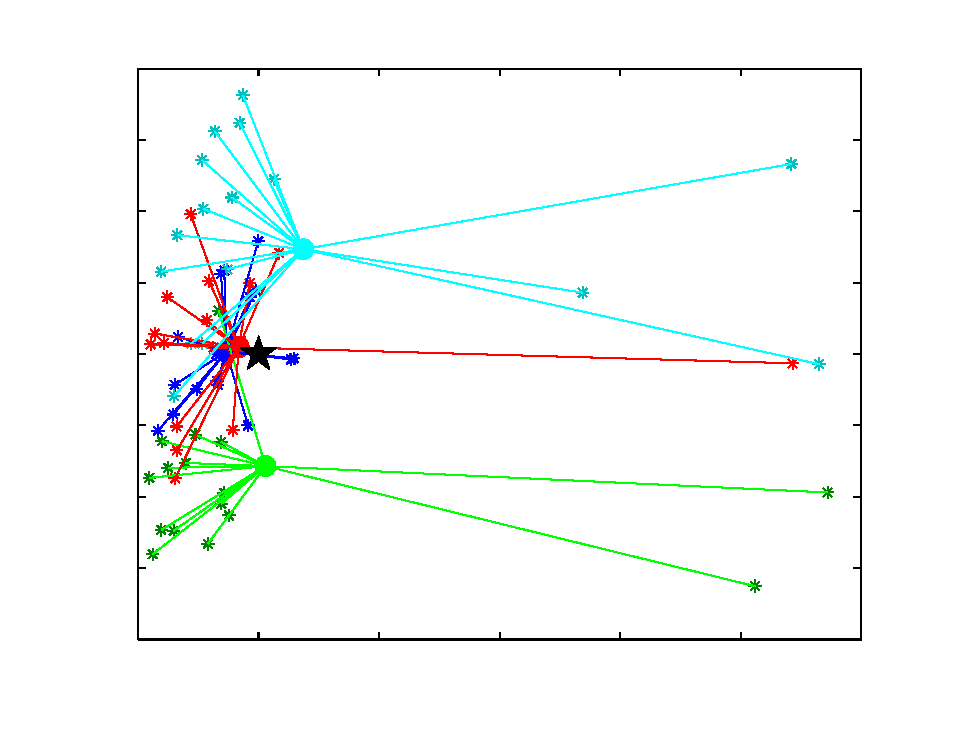
\includegraphics[width=1\textwidth]{Figures/tan_plan_2D_s16_b.eps}
%        %\subcaption{}
%        \label{fig:tan_plan_s16_a}
%      \end{minipage}
%      \begin{minipage}[b]{0.49\linewidth}
%        %\pgfimage[width=1\textwidth]{Figures/tan_plan_2D_s16_a-eps-converted-to.pdf}
%         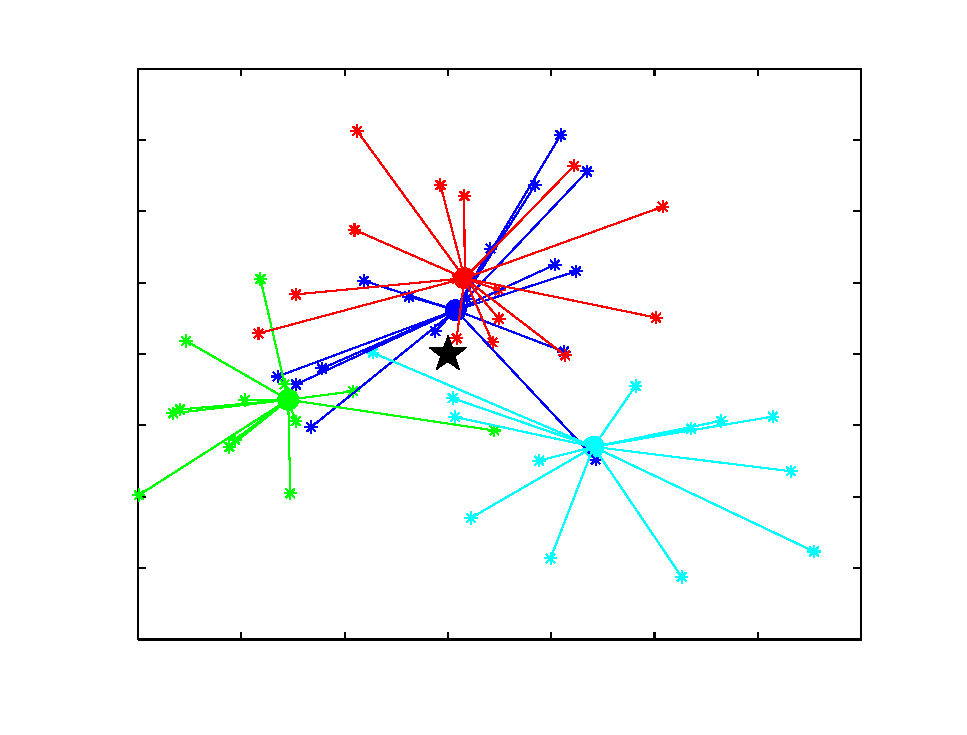
\includegraphics[width=1\textwidth]{Figures/tan_plan_2D_s16_a.eps}
%        %\subcaption{}
%        \label{fig:tan_plan_s16_b}
%      \end{minipage}
%      \begin{minipage}[b]{0.49\linewidth}
%        %\pgfimage[width=1\textwidth]{Figures/tan_plan_2D_s17_a-eps-converted-to.pdf}
%         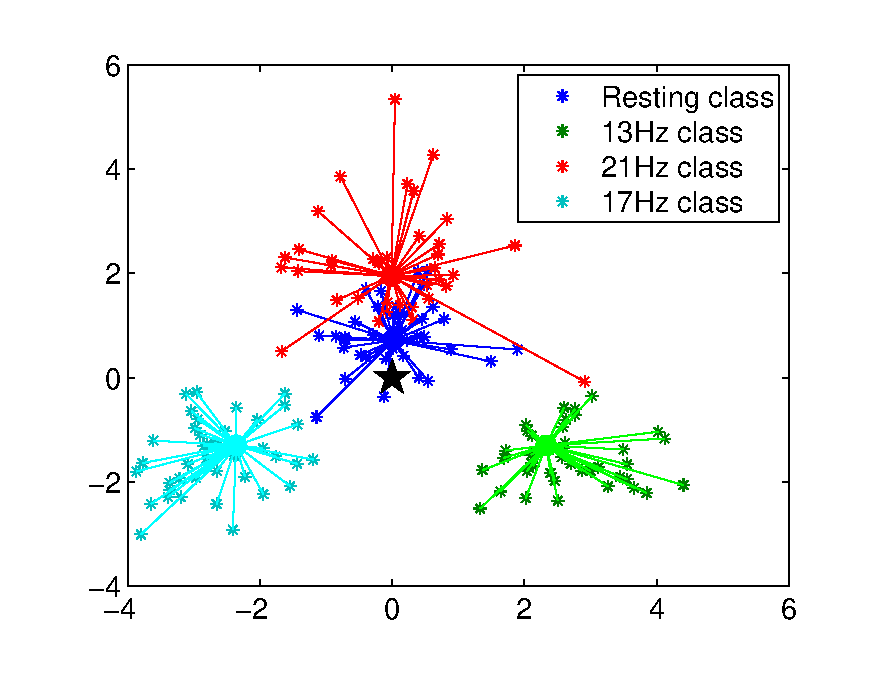
\includegraphics[width=1\textwidth]{Figures/tan_plan_2D_s17_a.eps}
%        %\subcaption{}
%        \label{fig:tan_plan_s17_a}
%      \end{minipage}
%      \begin{minipage}[b]{0.49\linewidth}
%        %\pgfimage[width=1\textwidth]{Figures/tan_plan_2D_s17_b-eps-converted-to.pdf}
%         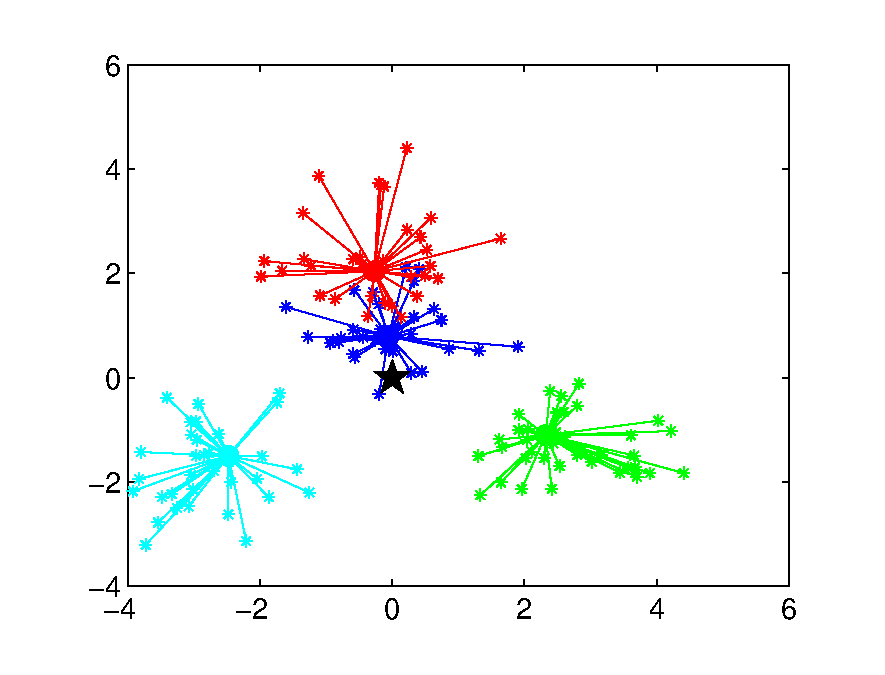
\includegraphics[width=1\textwidth]{Figures/tan_plan_2D_s17_b.eps}
%        %\subcaption{}
%        \label{fig:tan_plan_s17_b}
%        \end{minipage}
%        \caption{Scatter plot of covariance matrices for all trials mapped on the tangent space. The distance between each trial covariance matrix $\P_{\ti}$ and its Riemannian mean class $\P_{\Rm}^{(\ci)}$ is shown as connection line. The black star represents the Riemannian mean of all trials. % matrices regardless of their class. 
%Subject with lowest BCI performance, (\ref{fig:tan_plan_s16_a}) before and (\ref{fig:tan_plan_s16_b}) after Riemannian potato filtering. 
%Subject with highest BCI performance, (\ref{fig:tan_plan_s17_a}) before and (\ref{fig:tan_plan_s17_b}) after Riemannian potato filtering.}
%\label{fig:tan_plan_s16&17}
%% Sylvain: Est ce que c'est possible d'agrandir encore la patate Riemannienne pour eviter qu'il reste encore un outlier dans la classe 17Hz pour le sujet 16 (lowest BCI perfs, sur la Figure b) ? 
%%Emmanuel: Oui, mais la patate ne sera plus comme definit pas Barachant (a 2.5 x deviation standard). Elle est maintenant a 1.12 x deviation standard
%%Sylvain: Je pensais que les donnes serait plus etalee ainsi sur l'axe x, est possible de changer les valeur de debut et de fin du x-axis pour que les points des clusters soient repartis sur l'ensemble du plot ?
%%Emmanuel: Oui, c'est possible. Je l'avais fais ainsi pour que l'image garde le meme aspect. C'est fait! J'ai du aussi changer ma PCA. Elle influe beaucoup sur la disposition des points.
%%Sylvain: c'est normal. Les figures que tu as faites sont magnifiques !
%\end{figure}
\subsection{From Euclidean to Riemannian Centres of Class}
\label{subsec: from-euclid-to-riemann}

\begin{figure}[h!]
\centering
\subfigure[]{
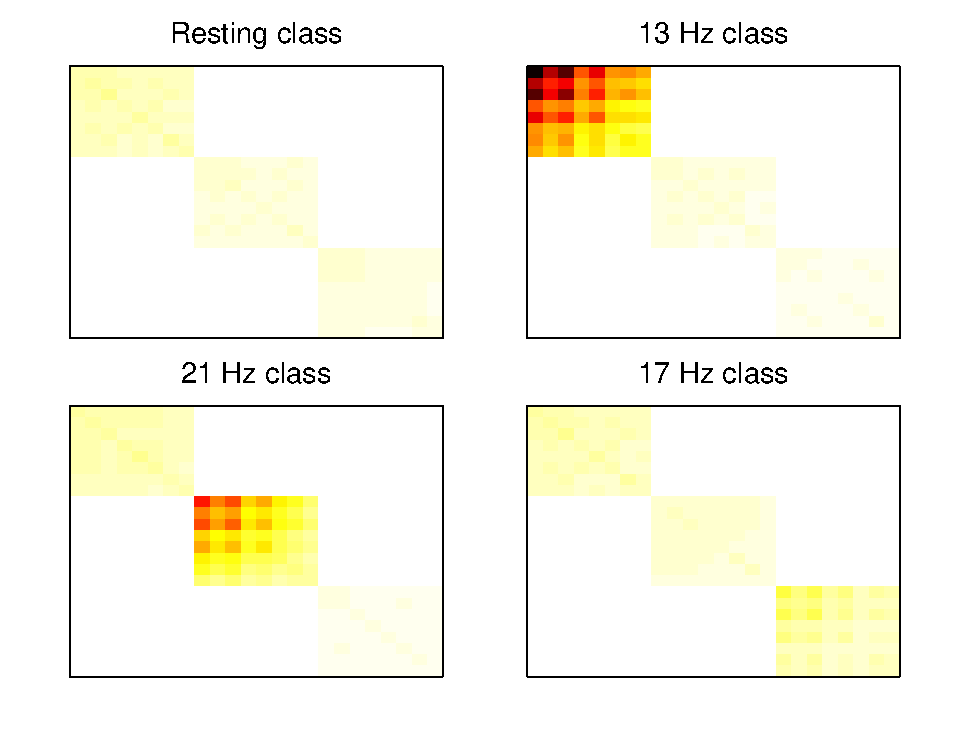
\includegraphics[width=0.47\textwidth]{Figures/covmat.eps}
\label{fig:covmat12}}
\subfigure[]{
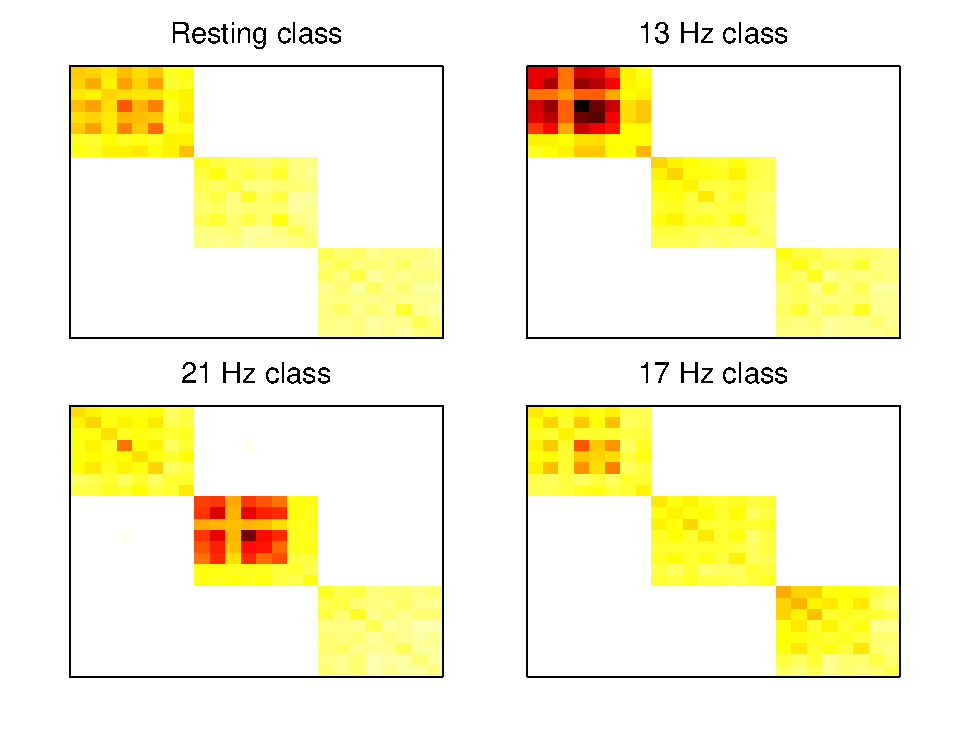
\includegraphics[width=0.47\textwidth]{Figures/covmat11.eps}
\label{fig:covmat11}}
\caption{Representation of covariance matrices: each image is the covariance matrix mean $\Pm^{(\ci)}$ of the class $\ci$, for one session of the recording. The diagonal blocks show the covariance in different frequency bands, i.e. 13 Hz in the upper-left block, 21 Hz in the middle, and 17 Hz in the bottom-right. Subjects with highest (a) and lowest (b) BCI performance. 
}
\label{fig:covmat}
\end{figure}

% The MDM classifier is simple. Once the covariance matrices have been estimated, the only major calculations involved are the mean and distance computations.
The covariance matrices obtained from SSVEP data extended with Eq.~\eqref{eq:ext_data} have interesting features, allowing the discrimination between signals of identical sources but with different frequencies. 
Figure~\ref{fig:covmat} shows the $K$ classes mean covariance matrices $\Pm^{(\ci)}$ from subjects with the highest (a) and lowest (b) classification accuracy. 
The three 8$\times$8 diagonal blocks hold the covariance matrices of the $\dF=3$ target frequencies.
Inter-frequencies covariance blocks are almost null.
In each mean covariance matrix, the block holding the covariance of the target frequency has the largest values. 
For the resting class, all $\dF$ blocks tend to have similar and small values. These features are more visible in the subject with the highest classification accuracy, and less visible in the one with lowest classification accuracy. 
It is interesting to see that features used for classification have a physiological meaning allowing an intuitive understanding, as opposed to \emph{black-boxes} approaches such as LDA or SVM. EEG processing complexity is encoded by the distance and not by machine learning.
% Contrary to discriminative classifiers classically used in BCI, such as LDA, SVM, etc, which appear as \emph{black-boxes} with difficult interpretation, it is very interesting to see that the presented covariance based classifier is based on features with an easy representation, and thus an intuitive understanding: the observed covariance matrices have a physiological meaning/interpretation.

Based on those covariance matrices, the different distances and means of Table~\ref{tab:dist} are compared in terms of classification accuracy and average CPU time elapsed on a trial classification, which involves the computation of four means of class and a distance to each mean.
Table~\ref{tab:res} summarises results obtained for each subject and each distance/divergence.
Euclidean distance yields drastically low accuracy. 
This support the fact that using Euclidean distance and Arithmetic mean on SPD matrices is not appropriate. 
This is generally attributed to the invariance under inversion and the fact that the determinant of the Arithmetic mean of SPD matrices can be larger than the determinant of its parts; it is referred to as the \textit{swelling effect}.
Since the value of the determinant is a direct measure of dispersion of the multivariate variables (i.e. EEG channels and frequency bands), it leads to poor discrimination in the classification task. 
The swelling effect of Arithmetic mean is shown in Figure~\ref{fig:swel}: the determinant of the Arithmetic mean is strictly larger than other means, the Log-Euclidean, Affine-Invariant and Bhattacharyya ones yielding similar determinants, close to trial values.
Another observation is that the Bhattacharyya distance and the S-divergence yield similar results. In the S-divergence section, it was stipulated the the square root of the S-Divergence was a distance, and it is seen here that it correspond to the Bhattacharyya distance.
%
%\begin{sidewaystable}[t]
%%\begin{table*}[t]
%\centering
%%\ra{1}
%\noindent\adjustbox{max width=\textwidth}{
%\begin{tabular}{c|c|c|c|c|c|c||c|c|c|c|c|c|c|c|c|c|c|c|c|c|}
%\cline{2-21}
%& \multicolumn{6}{ c||}{Euclidean} & \multicolumn{14}{ c| }{Riemannian} \\ \cline{2-21}
%& \multicolumn{2}{ c|}{Arithmetic}& \multicolumn{2}{ c|}{Harmonic}& \multicolumn{2}{ c||}{Geometric}&\multicolumn{2}{c|}{Log-Euclidean}&\multicolumn{2}{c|}{Affine-invariant}&\multicolumn{2}{c|}{$\alpha$-divergence}&\multicolumn{2}{c|}{Bhattacharyya}&\multicolumn{2}{c|}{Kullbacl-Leibler}&\multicolumn{2}{c|}{S-divergence}&\multicolumn{2}{c|}{Wassestein} \\ \cline{1-21}
%\multicolumn{1}{ |c| }{Sub.} & acc (\%) & time(s)& acc (\%) & time(s)& acc (\%) & time(s)& acc (\%) & time(s)& acc (\%) & time(s)& acc (\%) & time(s)& acc (\%) & time(s)& acc (\%) & time(s) & acc (\%) & time(s) & acc (\%) & time(s)\\ \hline
%\multicolumn{1}{ |c| }{1} & 53.12 & 0.025 & 48.44 & 0.015 & 00.00 & 0.000 & 71.88 & \textbf{0.150}& \textbf{73.44}& 0.194 & 			59.37 & 0.155 & 			68.75 & 			0.225 & 53.12 & 0.030 &  68.75  &  0.220  &  54.69  &  0.630\\ \hline
%\multicolumn{1}{ |c| }{2} & 43.75 & 0.020 & 31.25 & 0.025 & 00.00 & 0.000 & 78.13 & 		0.160 & 			79.69 & 0.190 &			79.69 & 0.200 & \textbf{81.25} & \textbf{0.065} & 54.69 & 0.045 & 81.25  &  0.255  &  54.69  &  0.285\\ \hline
%\multicolumn{1}{ |c| }{3} & 67.19 & 0.020 & 67.19 & 0.015 & 00.00 & 0.000 & 85.94 & 		0.120 &  		85.93 & 0.205 & \textbf{95.31} & 0.155 & 			85.94 & \textbf{0.100} & 71.88 & 0.060 & 85.94  &  0.200  &  76.56  &  0.280\\ \hline
%\multicolumn{1}{ |c| }{4} & 54.68 & 0.030 & 42.19 & 0.010 & 00.00 & 0.000 & 84.38 & 		0.225 &  		87.50 & 0.315 & \textbf{89.07} & 0.250 & 			85.94 & \textbf{0.100} & 48.44 & 0.025 & 85.94  &  0.120  &  65.62  &  0.310\\ \hline
%\multicolumn{1}{ |c| }{5} & 37.50 & 0.020 & 26.56 & 0.015 & 00.00 & 0.000 & 62.50 & \textbf{0.115}&  		68.75 & 0.290 & \textbf{73.44} & 0.140 & 			65.62 & 			0.125 & 67.19 & 0.030 & 65.63  &  0.110  &  45.31  &  0.660\\ \hline
%\multicolumn{1}{ |c| }{6} & 34.37 & 0.015 & 39.06 & 0.020 & 00.00 & 0.000 & 84.38 & 		0.120 & 			85.94 & 0.210 & \textbf{87.50} & 0.145 & 			82.81 & \textbf{0.100} & 62.50 & 0.030 & 82.81  &  0.130  &  53.13  &  0.300\\ \hline
%\multicolumn{1}{ |c| }{7} & 60.42 & 0.027 & 47.92 & 0.013 & 00.00 & 0.000 & 87.50 & 		0.267 &  		88.54 & 0.410 & \textbf{91.66} & 0.417 & 			86.46 & \textbf{0.137} & 54.17 & 0.043 & 86.46  &  0.243  &  69.79  &  0.777\\ \hline
%\multicolumn{1}{ |c| }{8} & 67.19 & 0.035 & 68.75 & 0.015 & 00.00 & 0.000 & 90.63 & 		0.215 & \textbf{92.19} & 0.290 & \textbf{92.19} & 0.290 &  \textbf{92.19}& \textbf{0.125} & 71.88 & 0.050 & 92.19  &  0.165  &  85.94  &  0.335\\ \hline
%\multicolumn{1}{ |c| }{9} & 57.81 & 0.035 & 42.19 & 0.015 & 00.00 & 0.000 & 70.31 &  		0.275 & 			70.31 & 0.380 & \textbf{75.00} & 0.300 & 			67.19 & \textbf{0.134} & 60.94 & 0.050 & 67.19  &  0.160  &  62.50  &  0.310\\ \hline
%\multicolumn{1}{ |c| }{10} & 38.28 & 0.035 & 28.12 & 0.013 & 00.00 & 0.000 & 75.00 & 		0.254 & 			80.47 & 0.514 & \textbf{82.03} & 0.510 & 			78.13 & \textbf{0.160} & 67.97 & 0.028 & 78.13  &  0.263  &  51.56  &  0.650\\ \hline
%\multicolumn{1}{ |c| }{11} & 48.44 & 0.025 & 46.88 & 0.010 & 00.00 & 0.000 & 60.94 & 		0.144 & 			65.63 & 0.235 & 			57.81 & 0.150 &  \textbf{75.00}& \textbf{0.105} & 39.06 & 0.040 & 75.00  &  0.195  &  56.25  &  0.575\\ \hline
%\multicolumn{1}{ |c| }{12} & 71.25 & 0.032 & 53.75 & 0.022 & 00.00 & 0.000 & 96.25 & \textbf{0.292}& 		96.69 & 0.534 & 			95.62 & 0.634 &  \textbf{96.88} & 		0.300 & 76.88 & 0.042 & 96.88  &  0.466  &  82.50  &  1.042\\ \hline \hline
%\multicolumn{1}{ |c| }{\textbf{Avg.}} & 52.83 & 0.027 & 45.19 & 0.016 & 00.00 & 0.000 & 78.98 & 0.194 & 81.27 & 0.314 & \textbf{81.56} & 0.279 & 80.51 & \textbf{0.140} & 60.72 & 0.039 & 80.51 &   0.210 & 63.21 & 0.513\\ \hline
%\end{tabular}
%}
%\caption{Subject classification accuracies (acc(\%)) and average CPU time (time(s)) elapsed for the classification of a single trial. Classification is performed with MDM using either Euclidean or Riemannian means (see Table~\ref{tab:dist}).}
%\label{tab:res}
%%\end{table*}
%\end{sidewaystable}


%%%%%%%%%%%%%%%%%%%%%%%%%%%%%%%%%%%%%%%%%%%%%%%%%%%%%%%%%%%%%%%%%%%%%%%%%%%%%%%%%%%%%%%%%%%%%%%%%%%%%%%%%%%%%%%%%%%%%%%%%%%
%\begin{sidewaystable}[t]
%%\begin{table*}[t]
%\centering
%%\ra{1}
%\noindent\adjustbox{max width=\textwidth}{
%\begin{tabular}{c|c|c|c|c|c|c||c|c|c|c|c|c|c|c|c|c|c|c|c|c|}
%\cline{2-21}
%& \multicolumn{6}{ c||}{Euclidean} & \multicolumn{14}{ c| }{Riemannian} \\ \cline{2-21}
%& \multicolumn{2}{ c|}{Arithmetic}& \multicolumn{2}{ c|}{Harmonic}& \multicolumn{2}{ c||}{Geometric}&\multicolumn{2}{c|}{Log-Euclidean}&\multicolumn{2}{c|}{Affine-invariant}&\multicolumn{2}{c|}{$\alpha$-divergence}&\multicolumn{2}{c|}{Bhattacharyya}&\multicolumn{2}{c|}{Kullbacl-Leibler}&\multicolumn{2}{c|}{S-divergence}&\multicolumn{2}{c|}{Wassestein} \\ \cline{1-21}

\begin{sidewaystable}[t]
%\begin{table*}[t]
\centering
\ra{1}
\noindent\adjustbox{max width=1.0\textwidth}{
\begin{tabular}{c|c|c|c|c|c|c||c|c|c|c|c|c|c|c|c|c|c|c|}
\cline{2-19}
& \multicolumn{4}{ c||}{Euclidean} & \multicolumn{14}{ c| }{Riemannian} \\ \cline{2-19}
& \multicolumn{2}{ c|}{Arithmetic}& \multicolumn{2}{ c|}{Harmonic}& \multicolumn{2}{c|}{Log-Euclidean}&\multicolumn{2}{c|}{Affine-invariant}&\multicolumn{2}{c|}{$\alpha$-divergence}&\multicolumn{2}{c|}{Bhattacharyya}&\multicolumn{2}{c|}{Kullback-Leibler}&\multicolumn{2}{c|}{S-divergence}&\multicolumn{2}{c|}{Wasserstein} \\ \cline{1-19}
\multicolumn{1}{ |c| }{Sub.} & acc (\%) & time(s) & acc (\%) & time(s) & acc (\%) & time(s)& acc (\%) & time(s)& acc (\%) & time(s)& acc (\%) & time(s)& acc (\%) & time(s) & acc (\%) & time(s) & acc (\%) & time(s)\\ \hline
\multicolumn{1}{ |c| }{1} & 53.12 & 0.025 & 40.62 & 0.030 & 71.88 & \textbf{0.150}& \textbf{73.44}& 0.194 & 			59.37 & 0.155 & 			68.75 & 			0.225 & 60.94 & 0.025 &  68.75  &  0.220  &  54.69  &  0.630\\ \hline
\multicolumn{1}{ |c| }{2} & 43.75 & 0.020 & 57.81 & 0.055 & 78.13 & 		0.160 & 			79.69 & 0.190 &			79.69 & 0.200 & \textbf{81.25} & \textbf{0.065} & 73.44 & 0.020 & 81.25  &  0.255  &  54.69  &  0.285\\ \hline
\multicolumn{1}{ |c| }{3} & 67.19 & 0.020 & 73.44 & 0.040 & 85.94 & 		0.120 &  		85.93 & 0.205 & \textbf{95.31} & 0.155 & 			85.94 & \textbf{0.100} & 95.31 & 0.040 & 85.94  &  0.200  &  76.56  &  0.280\\ \hline
\multicolumn{1}{ |c| }{4} & 54.68 & 0.030 & 50.312 & 0.030 & 84.38 & 		0.225 &  		87.50 & 0.315 & \textbf{89.07} & 0.250 & 			85.94 & \textbf{0.100} & 90.62 & 0.035 & 85.94  &  0.120  &  65.62  &  0.310\\ \hline
\multicolumn{1}{ |c| }{5} & 37.50 & 0.020 & 35.94 & 0.040 & 62.50 & \textbf{0.115}&  		68.75 & 0.290 & \textbf{73.44} & 0.140 & 			65.62 & 			0.125 & 70.31 & 0.035 & 65.63  &  0.110  &  45.31  &  0.660\\ \hline
\multicolumn{1}{ |c| }{6} & 34.37 & 0.015 & 62.50  & 0.035 & 84.38 & 		0.120 & 			85.94 & 0.210 & \textbf{87.50} & 0.145 & 			82.81 & \textbf{0.100} & 85.94 & 0.025 & 82.81  &  0.130  &  53.13  &  0.300\\ \hline
\multicolumn{1}{ |c| }{7} & 60.42 & 0.027 & 67.71  &  0.037 & 87.50 & 		0.267 &  		88.54 & 0.410 & \textbf{91.66} & 0.417 & 			86.46 & \textbf{0.137} & 94.79 & 0.020 & 86.46  &  0.243  &  69.79  &  0.777\\ \hline
\multicolumn{1}{ |c| }{8} & 67.19 & 0.035 & 78.12  &  0.035 & 90.63 & 		0.215 & \textbf{92.19} & 0.290 & \textbf{92.19} & 0.290 &  \textbf{92.19}& \textbf{0.125} & 95.31 & 0.030 & 92.19  &  0.165  &  85.94  &  0.335\\ \hline
\multicolumn{1}{ |c| }{9} & 57.81 & 0.035 & 43.75  &  0.035 & 70.31 &  		0.275 & 			70.31 & 0.380 & \textbf{75.00} & 0.300 & 			67.19 & \textbf{0.134} & 76.56 & 0.035 & 67.19  &  0.160  &  62.50  &  0.310\\ \hline
\multicolumn{1}{ |c| }{10} & 38.28 & 0.035 & 42.19  &  0.035 & 75.00 & 		0.254 & 			80.47 & 0.514 & \textbf{82.03} & 0.510 & 			78.13 & \textbf{0.160} & 82.81 & 0.045 & 78.13  &  0.263  &  51.56  &  0.650\\ \hline
\multicolumn{1}{ |c| }{11} & 48.44 & 0.025 & 48.44  &  0.030 & 60.94 & 		0.144 & 			65.63 & 0.235 & 			57.81 & 0.150 &  \textbf{75.00}& \textbf{0.105} & 48.44 & 0.030 & 75.00  &  0.195  &  56.25  &  0.575\\ \hline
\multicolumn{1}{ |c| }{12} & 71.25 & 0.032 & 63.12  &  0.040 & 96.25 & \textbf{0.292}& 		96.69 & 0.534 & 			95.62 & 0.634 &  \textbf{96.88} & 		0.300 & 94.37 & 0.040 & 96.88  &  0.466  &  82.50  &  1.042\\ \hline \hline
\multicolumn{1}{ |c| }{\textbf{Avg.}} & 52.83 & 0.027 & 55.56  &  0.037 & 78.98 & 0.194 & 81.27 & 0.314 & \textbf{81.56} & 0.279 & 80.51 & \textbf{0.140} & 80.74 & 0.040 & 80.51 &   0.210 & 63.21 & 0.513\\ \hline
\end{tabular}
}
\caption{Subject classification accuracy (acc(\%)) and average CPU time (time(s)) elapsed for the classification of a single trial. Classification is performed with MDM using either Euclidean or Riemannian means (see Table~\ref{tab:dist}).}
\label{tab:res}
%\end{table*}
\end{sidewaystable}
%%%%%%%%%%%%%%%%%%%%%%%%%%%%%%%%%%%%%%%%%%%%%%%%%%%%%%%%%%%%%%%%%%%%%%%%%%%%%%%%%%%%%%%%%%%%%%%%%%%%%%%%%%%%%%%%%%%%%%%%%%%








\begin{figure}[h!]
\centering
\subfigure[]{
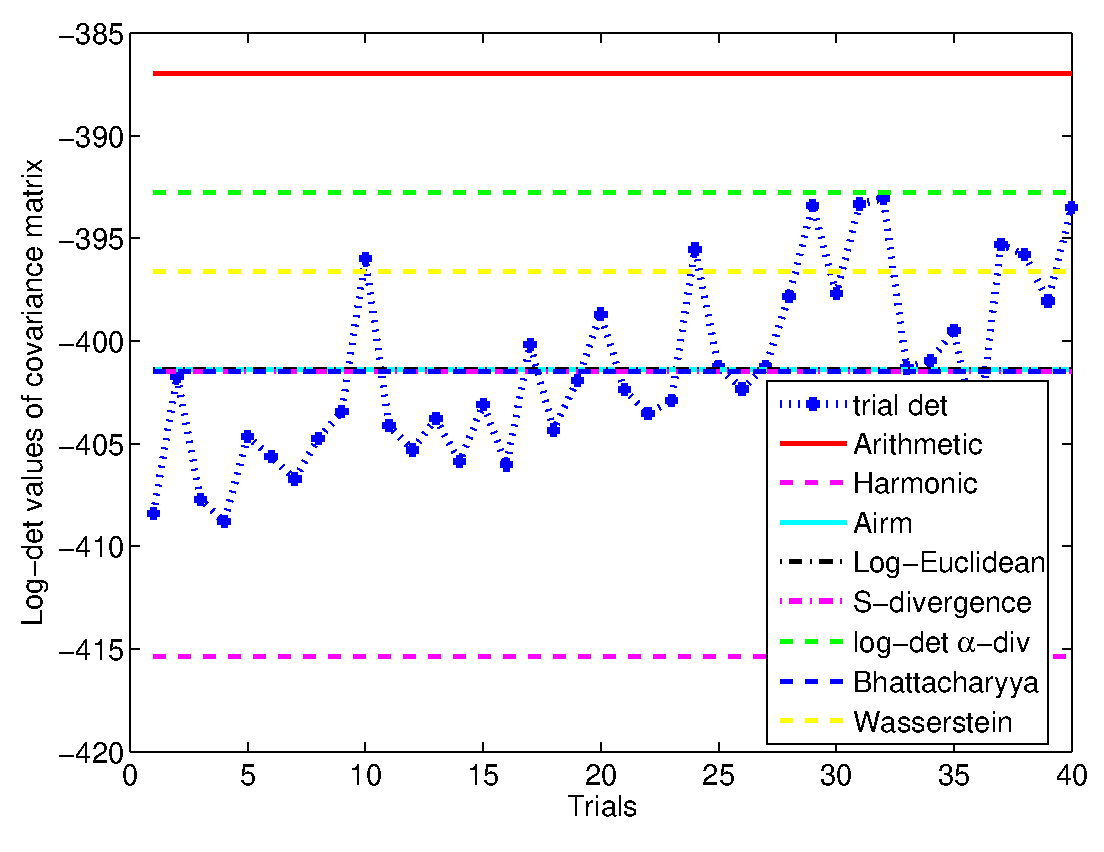
\includegraphics[width=0.46\textwidth]{Figures/swel.eps}
\label{fig:swel}
}
\subfigure[]{
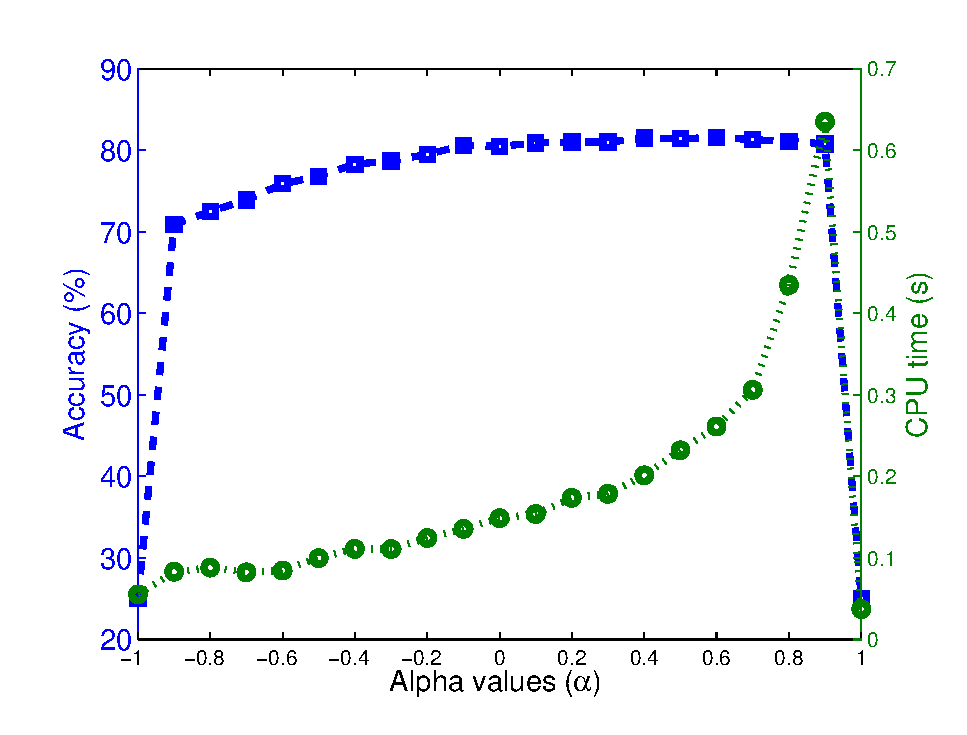
\includegraphics[width=0.49\textwidth]{Figures/alpha_cross.eps}
\label{fig:alphacross}
}
\caption{(a): Swelling effect of Arithmetic mean shown through log-determinant values. Training trials are taken from the 13 Hz class of the subject with the highest BCI performance. Log-determinant values are given for each trial covariance (points), and for means of Table~\ref{tab:dist} (horizontal lines). (b): Classification accuracy and CPU time, obtained with $\alpha$-divergence for $-1\leqslant \alpha  \leqslant 1$.} 
\label{fig:swel_alpha}
\end{figure} 

Riemannian distances significantly improve classification performances, with $\alpha$-divergence yielding the best results (81.56\%). 
The value of $\alpha$ was set to 0.6 through cross-validation. 
This procedure lasted 225.42 seconds and makes $\alpha$-divergence the most costly method, due to the optimisation of its parameter $\alpha$. 
Log-Euclidean yields lower classification accuracy (average 78.98\%) but could be computed faster than $\alpha$-divergence or Affine-Invariant distance.
However, the Bhattacharyya distance has the lowest computational cost of the considered Riemannian distances (average CPU time 0.140s), with a higher average accuracy of 80.51\%. 
So, it is a good trade-off between efficiency and speed. 
The accuracy and CPU time of the $\alpha$-divergence at different values of $\alpha$ are shown in Figure~\ref{fig:alphacross}.
It is seen that for $\alpha = \pm 1$, where $\alpha$-divergence represents a Bregman divergence associated with the log-determinant function, % also known as  log-det divergence, 
the classification accuracy are at the lowest accuracy (25\%). 
For all other values of alpha, the expected accuracy is 78.85$\pm$3.3\% and one can choose $-1 < \alpha < 1$ without any major impact on classification results.
%$\alpha$ could thus be fixed to any value between $\left]-1,+1\right[$ without causing drastic deterioration of accuracy. 
%For instance, the Bhattacharyya mean is equivalent to the $\alpha$-divergence mean with $\alpha$=0. 
This experiment on real EEG data shows that it is crucial to process covariance matrices with dedicated Riemannian tools, impacting the efficiency of the classification. 

\subsection{Classification Results and Analysis} % Classification Results
\label{sec:ssvep_response_delay}

In this section, the performance of the proposed method is presented.
First, the performance of the MDRM approach in an offline setup is analysed, then the results of the online algorithm are presented.
In the offline analysis, the relevance of identifying the latency between cue onset and SSVEP response is shown.
The results of the MDRM approach are compared to two state-of-the-art methods, \citep{lin_frequency_2006} and \citep{nakanishi_high-speed_2014}.
The online evaluation is divided in two parts: in the first one the algorithm discriminates between $\dK=\dF=3$ SSVEP classes (\textit{i.e.} 13, 17 and 21 Hz) and in the second one is applied on $\dK=4$ classes, \textit{i.e.} the $\dF=3$ SSVEP class and the resting class.

\subsubsection{Offline Analysis}
\label{sec:offline_analysis}
A close inspection of the filtered signals shows that almost all signals are synchronised with the trial frequency 2 seconds after cue onset $\cue = 0$, as shown in Figure~\ref{fig:sync_delay}.
This delay is mainly due to protocol design and user-specific cognitive processes.
The protocol is aimed to provide an asynchronous setup close to real applications. 
The user is not required to look at a fixation point or to directly gaze toward the target, as in \citep{kimura_ssvep-based_2013, nakanishi_high-speed_2014}, during inter-trial periods.
This is a tentative explanation for the higher delay observed in our study and it is consistent with literature observations \citep{vialatte_steady-state_2010, bakardjian_optimization_2010}

%synchronization for current trial frequency appears only 2 seconds after cue onset $\cue = 0$, as observed on Figure~\ref{fig:sync_delay}.
In fact, before $\cue + 2$s, for some users the signal could still be synchronised with the previous trial frequencies. 
An important increase in average classification accuracy (almost 10\%) could be obtained by taking the trial from 2 seconds after cue onset.
It is therefore crucial to consider the latency between the cue onset of trial and the actual synchronisation of SSVEP at stimulus frequency. 
Thus in the offline synchronous processing, the confident window for classification is set 2 seconds after the cue onset ($\cue+2$).
%1CL \begin{figure}[ht!]
%\begin{figure*}[ht!]
% 		\centering
% 		\begin{minipage}[b]{0.49\linewidth}
%          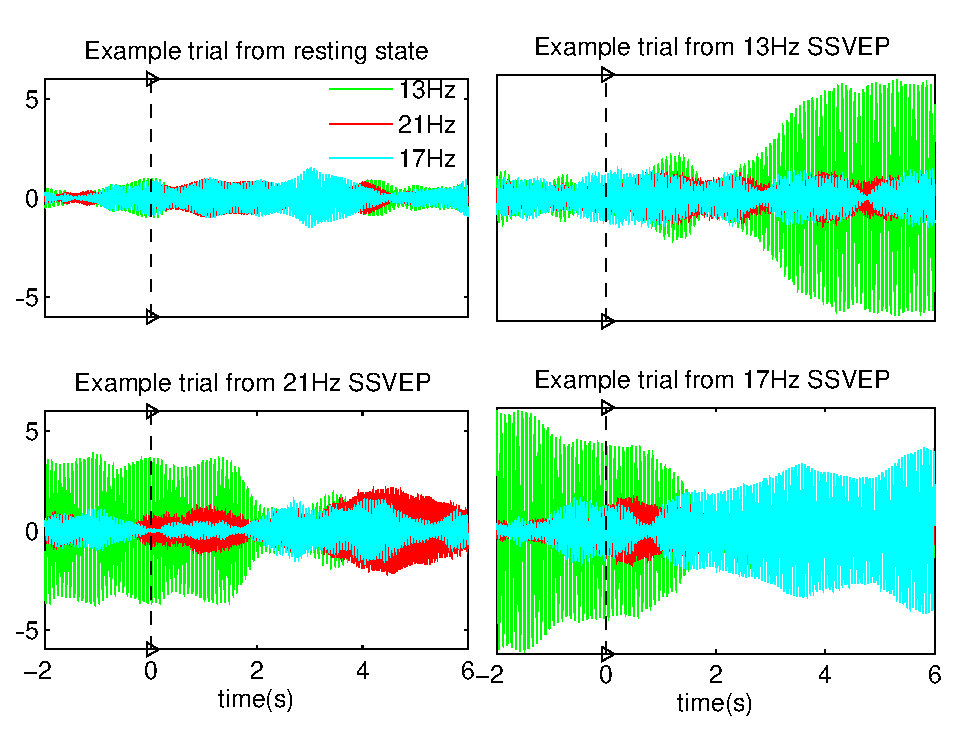
\includegraphics[width=1\textwidth]{Figures/ts17_f.eps}
%         \subcaption{} 
%		   \label{fig:sync_delay_best}
%         \end{minipage}    
% 		\begin{minipage}[b]{0.49\linewidth}
%          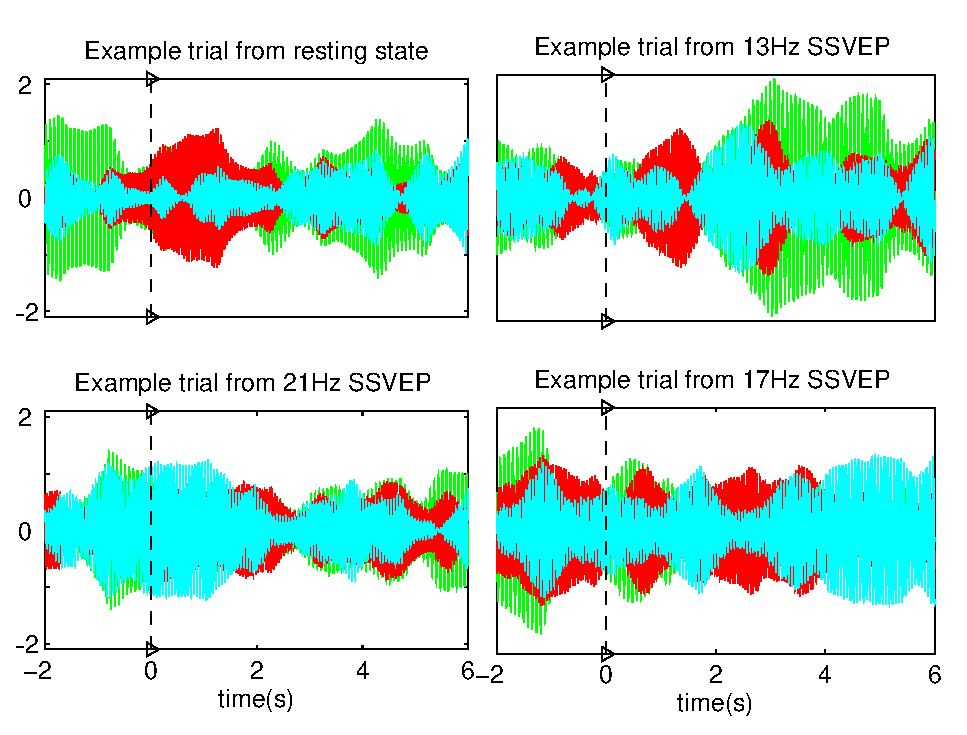
\includegraphics[width=1\textwidth]{Figures/ts16_f.eps}
%         \subcaption{}
%		  \label{fig:sync_delay_worst}
%         \end{minipage}
%         \caption{Signal amplitude at each stimulus frequency, showing synchronization of EEG with respect to time (seconds).
%         The raw signal of the trial measured on Oz is band filtered using a Butterworth of order 8 at each stimulus frequency and the resulting signals are shown in blue (dark grey), green (grey), and red (light grey) for the same signal filtered respectively at 13, 17, and 21Hz. 
%         The cue onset $\cue$ at time $0$ on the x-axis is shown with a vertical discontinued line. 
%         4 trials are shown, one for each class. Signals are from the subjects with the highest (\ref{fig:sync_delay_best}) and with the lowest BCI performance (\ref{fig:sync_delay_worst}).}
%         \label{fig:sync_delay}
%%1CL \end{figure}
%\end{figure*}
%***********************************
\begin{figure}[htb!]
\centering
\subfigure[]{
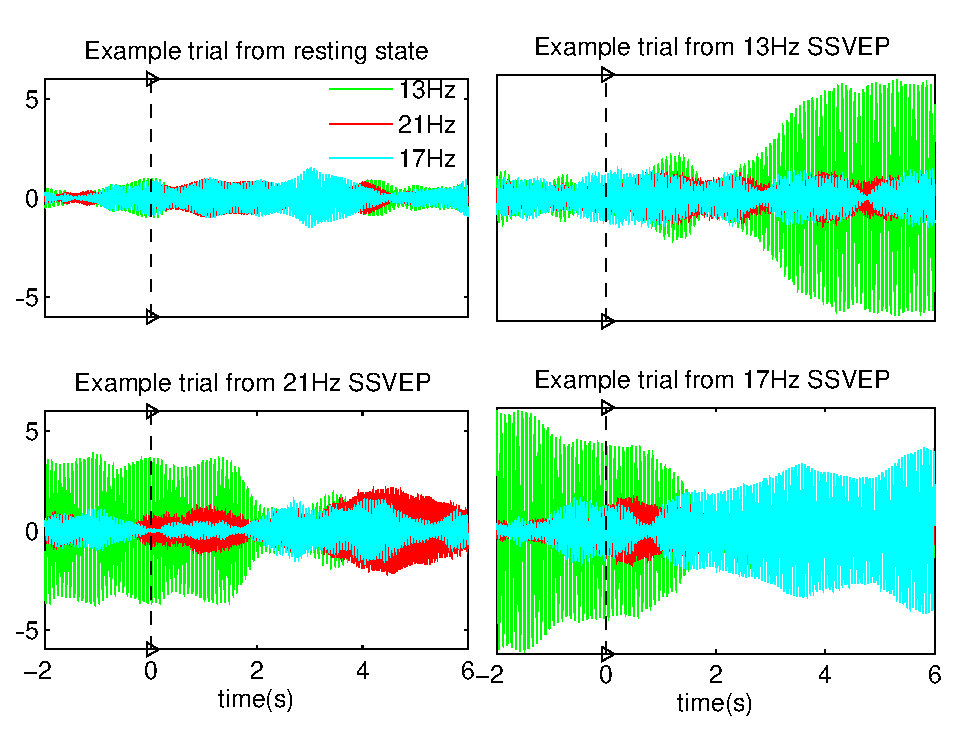
\includegraphics[width=0.6\textwidth]{Figures/ts17_f.eps}
\label{fig:sync_delay_best}
}
\subfigure[]{
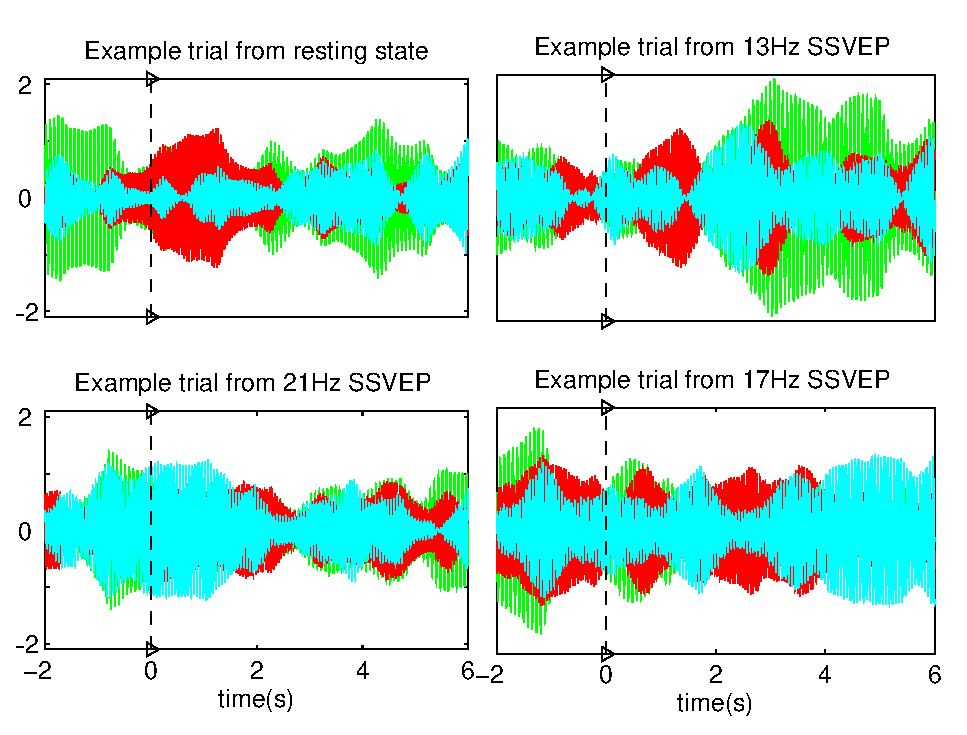
\includegraphics[width=0.6\textwidth]{Figures/ts16_f.eps}
\label{fig:sync_delay_worst}
}
\caption{Signal amplitude at each stimulus frequency, showing synchronisation of EEG with respect to time (seconds).
         The raw signal of the trial measured on Oz is band filtered using a Butterworth of order 8 at each stimulus frequency and the resulting signals are shown in blue (dark grey), green (grey), and red (light grey) for the same signal filtered respectively at 13, 17, and 21 Hz. 
         The cue onset $\cue$ at time $0$ on the x-axis is shown with a vertical discontinued line. 
         4 trials are shown, one for each class. Signals are from the subjects with the highest (\ref{fig:sync_delay_best}) and with the lowest BCI performance (\ref{fig:sync_delay_worst}).}
         \label{fig:sync_delay}
\end{figure}


Table~\ref{tab:res-offline} shows the offline classification accuracy for each subject obtained by the application of the \emph{MDRM} as described in Algorithm~\ref{alg:mdm}, with the epochs taken at $\cue+2$.
Column \emph{MDRM($\cue$)} shows the results obtained when the epochs are taken from cue onset.
The Riemannian potato technique presented in Section \ref{sec:potato} was applied for outlier removal (\emph{\mdrmpotato}).
The performance of the MDRM approach is compared to two CCA-based state-of-the-art methods %referred to as Lin and Nakanishi
proposed by \cite{lin_frequency_2006} and \cite{nakanishi_high-speed_2014} respectively.
In the implementation of these methods, the epochs are also taken from $\cue+2$.

The MDRM approach outperforms both CCA-based method with an average classification accuracy of 90.4$\pm$7.8 \% and ITR of 16.3$\pm$5.3 bits/min. 
\cite{lin_frequency_2006} ranks second with 87.5$\pm$15.1 \% and 15.5$\pm$6.8 bits/min. 
The method proposed by \cite{nakanishi_high-speed_2014}, which could be expected to achieve better results as reported in their work, only ranks third.
This is mainly due act that this method requires information on the phase of the stimuli. 
% SSVEP trials belonging to a unique class should not only be synchronised at the same frequency, they should be in-phase.
% To ensure this, a more rigid experimental setting is needed, where the beginning of the flash stimuli are controlled by a computer and tightly linked to the trial cue onset. 
% The experimental setting used in this work are more flexible and simple; they do fix the phase of the SSVEP response. 
In fact, \cite{nakanishi_high-speed_2014} use the average of all training trials belonging to a unique class as a reference signal in the CCA.
When SSVEP trials belonging to a unique trial are not in-phase, which is the case in the current work, averaging them will cancel the signal.

Within the MDRM approach, it is shown that taking into account the latency between the cue onset and the SSVEP response significantly increases the classification performances: accuracy and ITR rise from 75.9$\pm$11.4\% and 6.0$\pm$3.1 bits/min to 90.4$\pm$7.8\% and 16.3$\pm$5.3 bits/min.
In turn removing outliers with the Riemannian potato does not bring significant change.
This could be attributed to the fact that the recording have been conducted in controlled environment, with small or little external noise.  


%This table shows that synchronous applications give better results, which is due to the fact that require extra information, \textit{i.e.} cue onsets. %but they are very limited in term of user interaction.
%Columns ``Online'' and ``Online + $\disvec_{\cloutmp}$'' contain the performance of the online algorithm as described in Algorithm~\ref{alg:online}.
%For the offline approaches, classification is only done at the end of the trial, that is 3.6 seconds after cue onset and 5.6 after cue onset for ``offline opt.''.

\begin{table*}[ht!]
\centering
\ra{1}
\begin{adjustbox}{center}
\resizebox{1.2\textwidth}{!}{
%1CL \resizebox{1.2\textwidth}{!}{
\begin{tabular}{c||c|c||c|c||c|c||c|c||c|c||}
\cline{2-11}
&  \multicolumn{10}{|c||}{Offline algorithms}\\
\cline{2-11}
&  \multicolumn{2}{ c||}{Lin \textit{et al.} } & \multicolumn{2}{|c||}{Nakanishi \textit{et al.} } & \multicolumn{2}{|c||}{MDRM($\cue$)} & \multicolumn{2}{|c||}{MDRM} & \multicolumn{2}{|c||}{\mdrmpotato} \\ \cline{2-11}
     &   acc(\%) & itr(bpm) &   acc(\%) & itr(bpm) &   acc(\%) & itr(bpm) &   acc(\%) & itr(bpm) &   acc(\%) & itr(bpm) \\ \hline
\multicolumn{1}{ |c|| }{  S1} &     91.7 &     16.3 &     84.7 &     12.2 &     67.6 &      3.5 &     84.7 &     12.2 &     84.5 &     12.1 \\ \hline
\multicolumn{1}{ |c|| }{  S2} &     45.8 &      0.7 &     47.9 &      1.0 &     66.0 &      3.2 &     79.4 &      9.7 &     79.3 &      9.6 \\ \hline
\multicolumn{1}{ |c|| }{  S3} &    100.0 &     23.8 &     93.0 &     17.2 &     90.2 &     10.3 &     99.3 &     22.7 &     99.3 &     22.7 \\ \hline
\multicolumn{1}{ |c|| }{  S4} &     97.9 &     21.3 &     96.6 &     20.0 &     78.3 &      6.1 &     89.7 &     15.0 &     89.7 &     15.0 \\ \hline
\multicolumn{1}{ |c|| }{  S5} &     83.3 &     11.5 &     82.2 &     11.0 &     76.0 &      5.5 &     89.5 &     14.9 &     89.4 &     14.9 \\ \hline
\multicolumn{1}{ |c|| }{  S6} &     77.1 &      8.7 &     76.2 &      8.3 &     72.2 &      4.5 &     87.2 &     13.6 &     87.2 &     13.6 \\ \hline
\multicolumn{1}{ |c|| }{  S7} &     98.6 &     22.0 &     96.7 &     20.1 &     90.0 &     10.2 &     99.8 &     23.5 &     99.8 &     23.4 \\ \hline
\multicolumn{1}{ |c|| }{  S8} &     97.9 &     21.3 &     65.5 &      4.7 &     90.4 &     10.3 &     99.7 &     23.2 &     99.7 &     23.2 \\ \hline
\multicolumn{1}{ |c|| }{  S9} &     91.7 &     16.3 &     77.9 &      9.0 &     64.0 &      2.8 &     85.8 &     12.8 &     85.7 &     12.7 \\ \hline
\multicolumn{1}{ |c|| }{ S10} &     80.2 &     10.0 &     76.9 &      8.6 &     79.2 &      6.4 &     93.1 &     17.3 &     93.0 &     17.2 \\ \hline
\multicolumn{1}{ |c|| }{ S11} &     89.6 &     15.0 &     82.7 &     11.2 &     54.8 &      1.4 &     78.2 &      9.2 &     78.2 &      9.1 \\ \hline
\multicolumn{1}{ |c|| }{ S12} &     95.8 &     19.4 &     93.8 &     17.8 &     82.3 &      7.4 &     98.6 &     22.0 &     98.6 &     22.0 \\ \hline
\multicolumn{1}{ |c|| }{\textbf{Mean}} &     \textbf{87.5$\pm$15.1} &     \textbf{15.5$\pm$6.8} &     \textbf{81.2$\pm$14.1} &     \textbf{11.8$\pm$6.0} &     \textbf{75.9$\pm$11.4} &      \textbf{6.0$\pm$3.1} &     \textbf{90.4$\pm$7.8} &     \textbf{16.3$\pm$5.3} &     \textbf{90.4$\pm$7.8} &     \textbf{16.3$\pm$5.3} \\ \hline
\end{tabular}
}
\end{adjustbox}
\caption{Offline performance in terms of accuracy and ITR. Five methods are compared: (1) CCA approach introduced by \citep{lin_frequency_2006}, (2) CCA approach introduced by \citep{nakanishi_high-speed_2014}, (3) MDRM described in Section \ref{subsec:mdm} (Algorithm \ref{alg:mdm}), (4) MDRM where processed epochs are taken 2 seconds from the beginning of the trial, and (5) \mdrmpotato, where outliers are removed using the Riemannian potato approach described in Section~\ref{sec:potato}.}
\label{tab:res-offline}
\end{table*}


%\begin{table*}[ht!]
%\centering
%\ra{1}
%\begin{tabular}{c|c|c|c|c|}
%\cline{2-5}
%&  \multicolumn{2}{ c|}{Offline} &\multicolumn{2}{ c| }{Offline opt.} \\ \cline{1-5}
%\multicolumn{1}{ |c| }{Sub.} & acc & ITR  & acc & ITR \\ \hline
%\multicolumn{1}{ |c| }{1} & 62.50 & 7.52 & 73.44 & 7.97 \\ \hline
%\multicolumn{1}{ |c| }{2} & 67.19 & 9.45 & 79.69 & 10.18 \\ \hline
%\multicolumn{1}{ |c| }{3} & 85.94 & 19.86 & 85.94 & 12.76 \\ \hline
%\multicolumn{1}{ |c| }{4} & 78.12 & 14.92 & 87.50 & 13.48 \\ \hline
%\multicolumn{1}{ |c| }{5} & 70.31 & 10.87 & 68.75 & 6.52 \\ \hline
%\multicolumn{1}{ |c| }{6} & 79.69 & 15.83 & 85.94 & 12.76 \\ \hline
%\multicolumn{1}{ |c| }{7} & 78.12 & 14.92 & 88.54 & 13.98 \\ \hline
%\multicolumn{1}{ |c| }{8} & 89.06 & 22.14 & 92.19 & 15.86 \\ \hline
%\multicolumn{1}{ |c| }{9} & 62.50 & 7.52 & 70.31 & 6.98 \\ \hline
%\multicolumn{1}{ |c| }{10} & 60.94 & 6.93 & 80.47 & 10.48 \\ \hline
%\multicolumn{1}{ |c| }{11} & 43.75 & 2.00 & 65.62 & 5.64 \\ \hline
%\multicolumn{1}{ |c| }{12} & 80.00 & 16.02 & 96.88 & 18.75 \\ \hline \hline
%\multicolumn{1}{ |c| }{Average} & 71.51 & 12.33 & 81.27 & 11.28 \\ \hline
%\multicolumn{1}{ |c| }{std} & 12.82 & 5.91 & 9.93 & 4.03 \\ \hline
%\end{tabular}
%\caption{Average classification accuracies (acc) achieved using the state-of-the-art MDRM (Offline) and the optimized version of the MDRM (Offline opt.) where processed epoch is taken 2 seconds from the beginning of the trial. Their corresponding ITR are also provided.}
%%\caption{Average classification accuracy for each subject and time delay, from beginning of trial $t_0$, before valid classification output. The results obtained when using the cue onset $t_0$ as time reference and a fixed 2-seconds delay (synchronous) are compared to the results where no time reference is used (asynchronous), and enhanced by $\disvec_j$ (asynchronous + $\disvec_j$).}
%\label{tab:res-offline}
%\end{table*}


%It is divided into two parts: first, the relevance of identifying the latency between cue onset and SSVEP response is shown through the evaluation of the impact of SSVEP delays considered for offline classification. Then, performances of offline and online algorithms are compared and analysed. 
%\subsubsection{SSVEP Response Time Delay for Offline}
% \label{sec:ssvep_response_delay}

%Figure~\ref{fig:sync_delay} shows time signals of one trial from each class, measured at $Oz$, for the subject with highest BCI performance and for the subject with lowest BCI performance. 
%The figure displays the raw signal filtered at the 3 different stimulus frequency, each with a different color: 13Hz in blue, 17Hz in red, 21Hz in green.
%%The signal is replicated 3 times with each replicate being the raw signal filtered at a different stimulus frequency. Each replicate is shown in a different color. 
% It is visible that synchronization for current trial frequency appears only 2 seconds after cue onset $\cue = 0 s$ on the $x$-axis of the plots.
% In fact, before $\cue + 2$ seconds the signal is still synchronized with the previous trial frequencies. 
% In the signals from the subject with the highest BCI performance, synchronization at the trial stimulus frequency is predominant and permanent after $\cue + 2$, which eases the classification task. 
% Moreover, for the resting trial (no SSVEP), the power in all stimuli frequencies is sensibly decreased. 
% However, the poor predictive capability for the subject with lowest BCI performance could be explained by the fact that the predominance of the trial stimulus frequency is not always evident and not permanent. 
% Also, during the resting trial, the power in stimuli frequencies is not significantly decreased.    
% \begin{figure}[ht!]
% 		\centering
% 		\begin{minipage}[b]{0.9\linewidth}
%          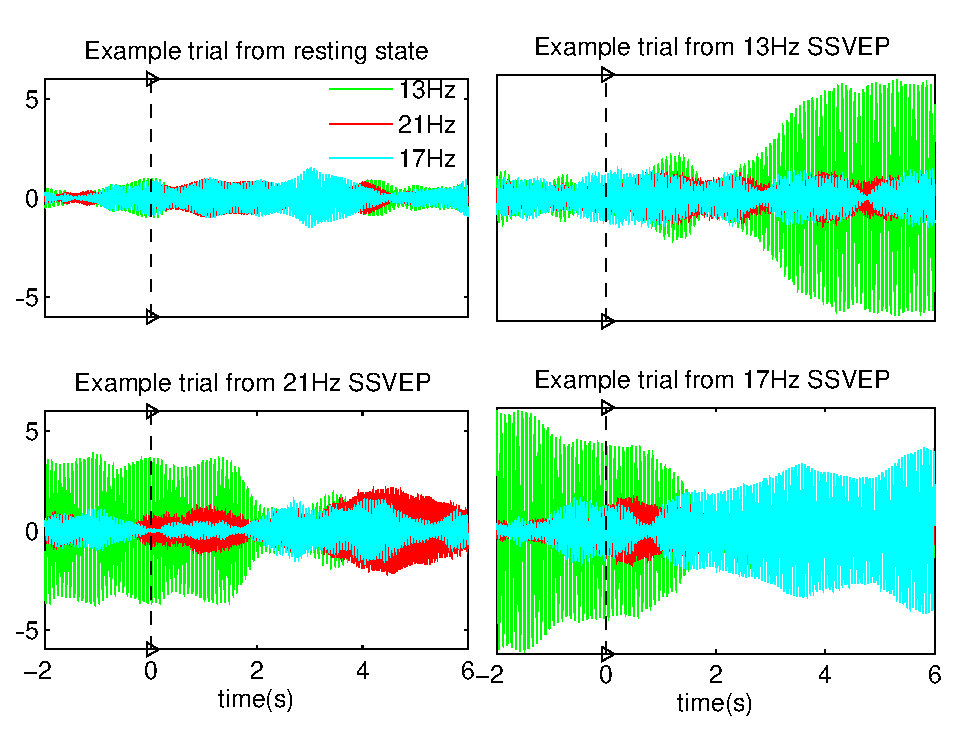
\includegraphics[width=1\textwidth]{Figures/ts17_f.eps}
%         \subcaption{Example of trials for the subject with the highest BCI performance}
%         \end{minipage}
        
% 		\begin{minipage}[b]{0.9\linewidth}
%          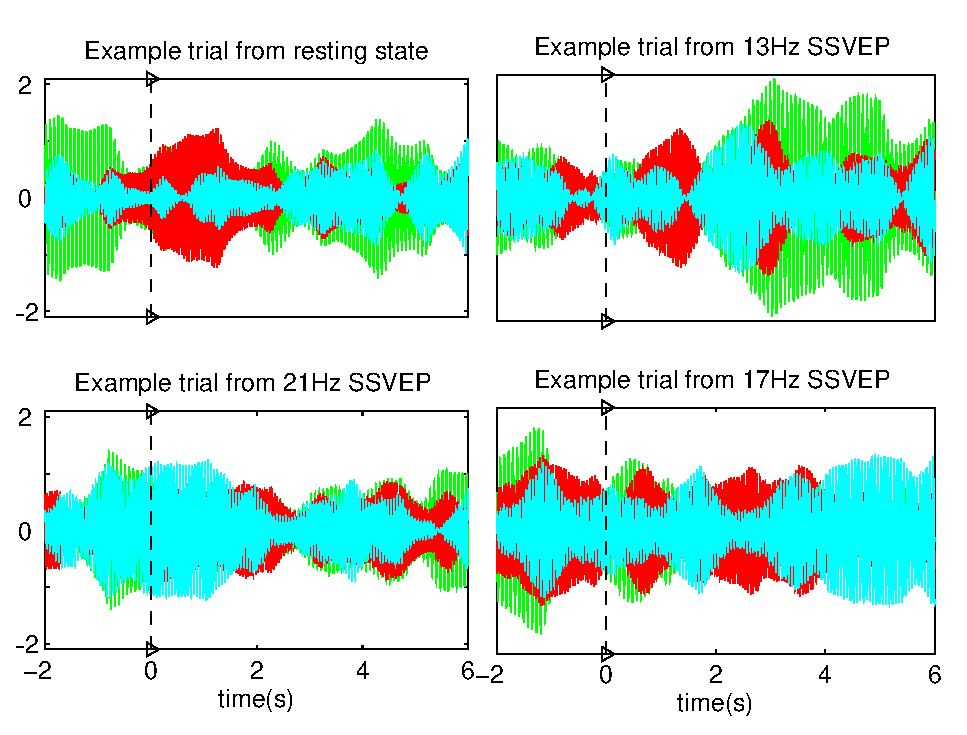
\includegraphics[width=1\textwidth]{Figures/ts16_f.eps}
%         \subcaption{Example of trials for the subject with the lowest BCI performance}
%         \end{minipage}
%         \caption{Signal amplitude at each stimulus frequency, showing synchronization of EEG with respect to time (seconds). The raw signal of the trial measured on Oz is band filtered using a Butterworth of order 8 at each stimulus frequency and the resulting signals are shown in blue (dark grey) , green (grey), and red (light grey) for the same signal filtered respectively at 13, 17, and 21 Hz. The cue onset $\cue$ at time $0$ on the x-axis is shown with a vertical discontinued line. 4 trials are shown, one for each class. Signals from the subjects, (a) with highest BCI performance and (b) with lowest BCI performance.}
%         \label{fig:sync_delay}
% \end{figure} 

% Similar observation is made from Figure~\ref{fig:sync_delay_psd} where the time-frequency representations of EEG trials per class are plotted for the subjects with the highest and lowest BCI performances. % 11 (a) and 12 (b).
% The time-frequency representation is obtained with a STFT on rectangular windowing.
% Each plot has 4 rows, one for each class, displaying the power spectral density (averaged over all trials) in the 13Hz, 17Hz, and 21Hz frequency bands as a function of the trial time.
% \begin{figure}[ht!]
% 		\centering
% 		\begin{minipage}[b]{0.8\linewidth}
%         \pgfimage[width=1\textwidth]{Figures/mPSD_s17-eps-converted-to.pdf}
%          %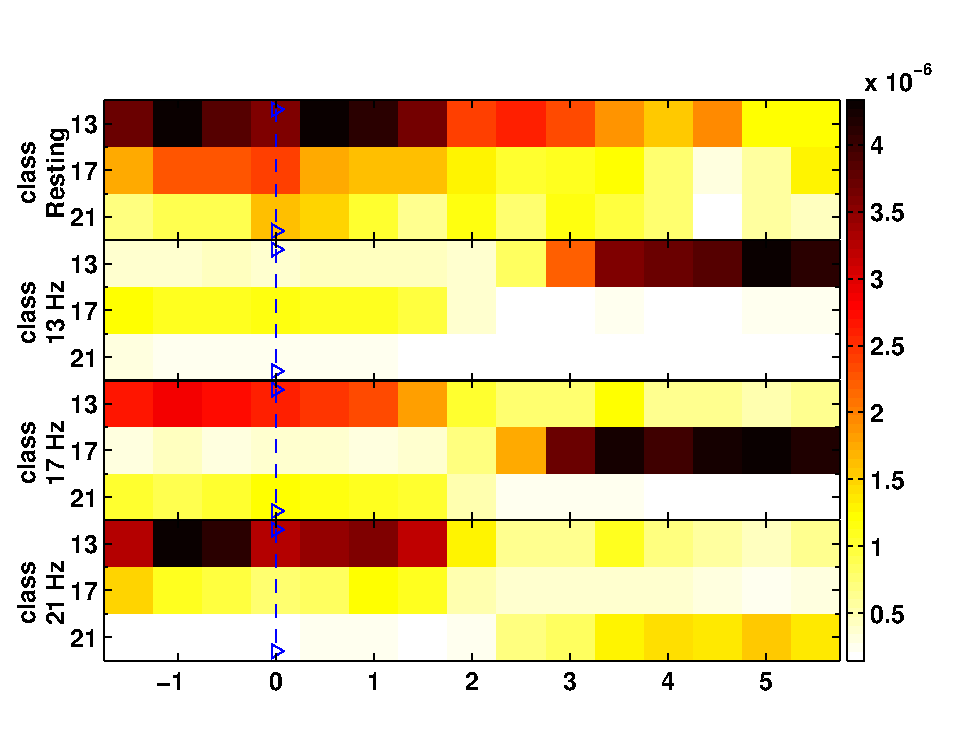
\includegraphics[width=1\textwidth]{Figures/mPSD_s17.eps}
%         \subcaption{Time-frequency diagrams for the subject with the highest BCI performance}
%         \end{minipage}
        
%         \begin{minipage}[b]{0.8\linewidth}
%         \pgfimage[width=1\textwidth]{Figures/mPSD_s16-eps-converted-to.pdf}
%          %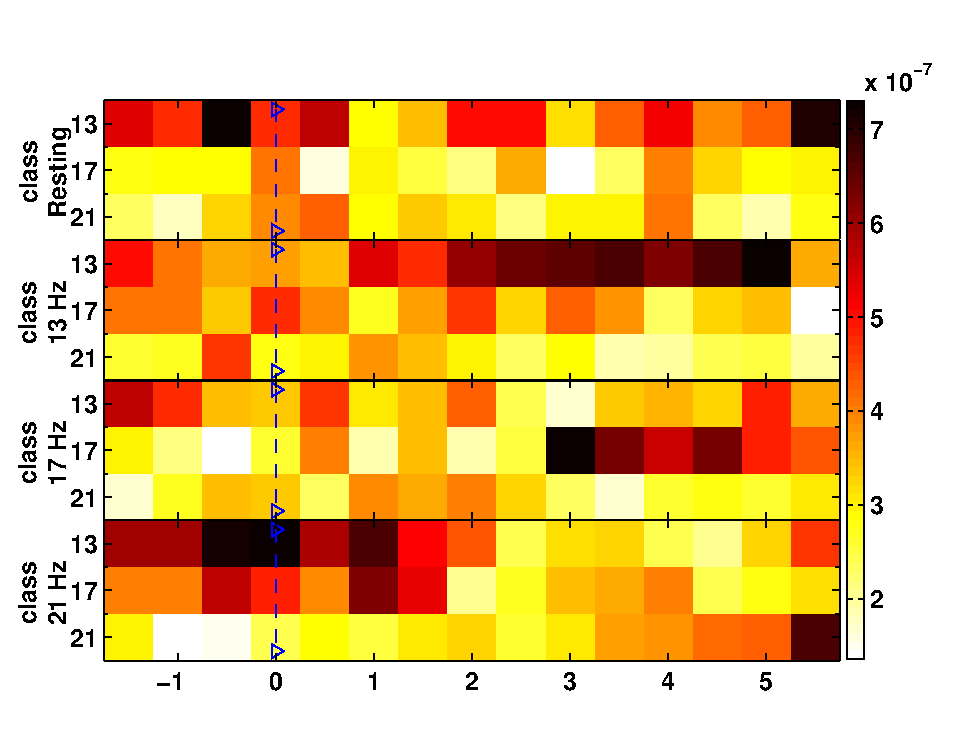
\includegraphics[width=1\textwidth]{Figures/mPSD_s16.eps}
%         \subcaption{Time-frequency diagrams for the subject with the lowest BCI performance}
%         \end{minipage}
%         \caption{Time-frequency representation of EEG from various classes showing synchronization at in frequency bands (indicated on y axis) on both side of the cue onset. The power of synchronization is shown in the color bar. Dark colors show strong synchronization. 4 trials (top to bottom) are represented, one for each class. Signals from the subjects, (a) with highest BCI performance and (b) with lowest BCI performance.}
%         \label{fig:sync_delay_psd}
% \end{figure}

% An important increase in average classification accuracy (almost 10\%) could be obtained by taking the trial from 2 seconds after cue onset.
% % Considering the delay between the cue onset and the synchronization in the appropriate frequency band by taking the EEG sample after 2 second after cue onset brings an increase in the average classification accuracy of up to 15\%. 
% It is therefore crucial to consider the latency between the trial's cue onset and the actual synchronization of SSVEP at stimulus frequency. 
%locate the EEG signal window where classification results have the high confidence, while maintaining a decent response time in the system.
% without inserting a too long delay in the system response time.   
%\textcolor{red}{Attention: reprendre la fin de cette section. On a l impression de faire du online optimis\'e. De plus, ce paragraphe ne devrait pas etre dans la section "Online Classification".}
%\subsubsection{Online Classification Results}
%Code: 	SSVEP_Riemannian_multiclass.m: For synchronous results
%		SSVEP_Riemannian_multiclass_cumulative.m: For asyncchronous 
%		SSVEP_Riemannian_multiclass_cumulative_curve.m: For asyncchronous (+ gradient curve) results
%		SSVEP_Riemannian_multiclass.m: For offline opt.
%		SSVEP_Riemannian_multiclass.m: For offline (state of the art).
%		SSVEP_Riemannian_multiclass_naive.m: For raw application of MDRM on online and asych (naive)

\subsubsection{Online Analysis without Resting Class}

In an online asynchronous experiment, there is no cue onset, and the delay before SSVEP synchronisation might differ from one trial to another and from one subject to another. 
To locate the trust EEG region for the classification, $\dd$ and $\pthres$ are set respectively to 5 and 0.7 through cross-validation. 
The performance of this online setup is analysed and Figure~\ref{fig:probErrorEpochs} shows the results. 
From the analysis shown in Figure~\ref{fig:accaracy_tlen}, the epoch size is set to $\ws = 2.6 $ seconds.
The step size is set to $\deltaN = 0.2$s, that is a new epoch is classified every $0.2$ second.

On Figure~\ref{fig:classErrorEpochs}, the classification error is plotted against the epoch index. 
It shows that the error decreases as epochs move from the beginning of the trial.
The error increases in the last epochs of the trial, corresponding to the end of the SSVEP task.  
%The classification is performed as described in Algorithm \ref{alg:online} up to step \ref{op3:get_rho} and $\cloutmp$ is considered as the output. No probability threshold and no curve direction are used for the validation of this output. 
%epochs moves from the beginning of the trial. 
Figure~\ref{fig:classProbEpochs} details the evolution of the probability for each class as epochs index increases. 
% how the probability of the actual class varies along the trial. 
It appears clearly that the class of the EEG trial (thick-and-star line) has the largest probability only a few epochs after the beginning of the trial. 
Moreover, one can see that this is an increasing trend over the whole trial. 
%It is seen that the actual class has the largest probability only few epochs after the beginning of the trial and has an increasing trend. 
Thus by setting an appropriate probability threshold $\pthres$, the actual class can be identified with enough confidence.  
Figure~\ref{fig:errorProbTresh} shows the influence of the probability threshold $\pthres$ on the classification error. 
The error is reduced when the probability threshold $\pthres$ is increased. 
Figure~\ref{fig:accaracy_tlen} shows how the average online performance varies with respect to the epoch size ($\ws$).
Both the classification accuracy and the ITR are shown. 
With short $\ws$ values, the epoch size does not capture enough feature for a correct classification, and with long $\ws$, the epoch losses temporal resolution.
The ITR increases with the classification rate but drops sensibly after a peak value. 

%\begin{figure}[ht!]
%		\centering
%		\begin{minipage}[b]{0.48\linewidth}
%         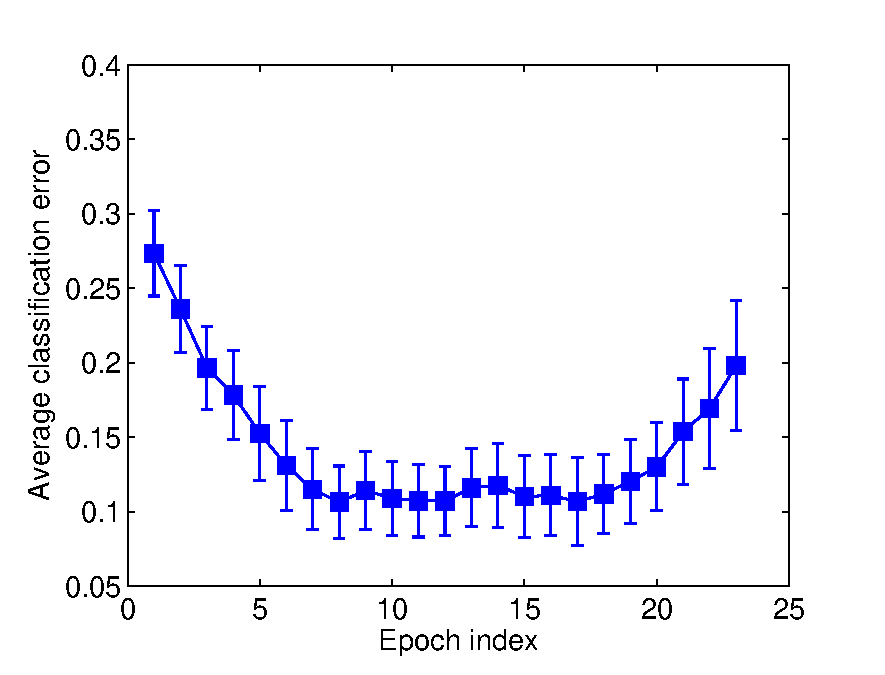
\includegraphics[width=1\textwidth]{Figures/classError_epochs.eps}
%        %\pgfimage[width=1\textwidth]{Figures/classError_epochs.eps}
%        \subcaption{ }
%        \label{fig:classErrorEpochs}
%      \end{minipage}      
%      \begin{minipage}[b]{0.48\linewidth}
%        %\pgfimage[width=1\textwidth]{Figures/classProb_epochs_s12.eps}
%         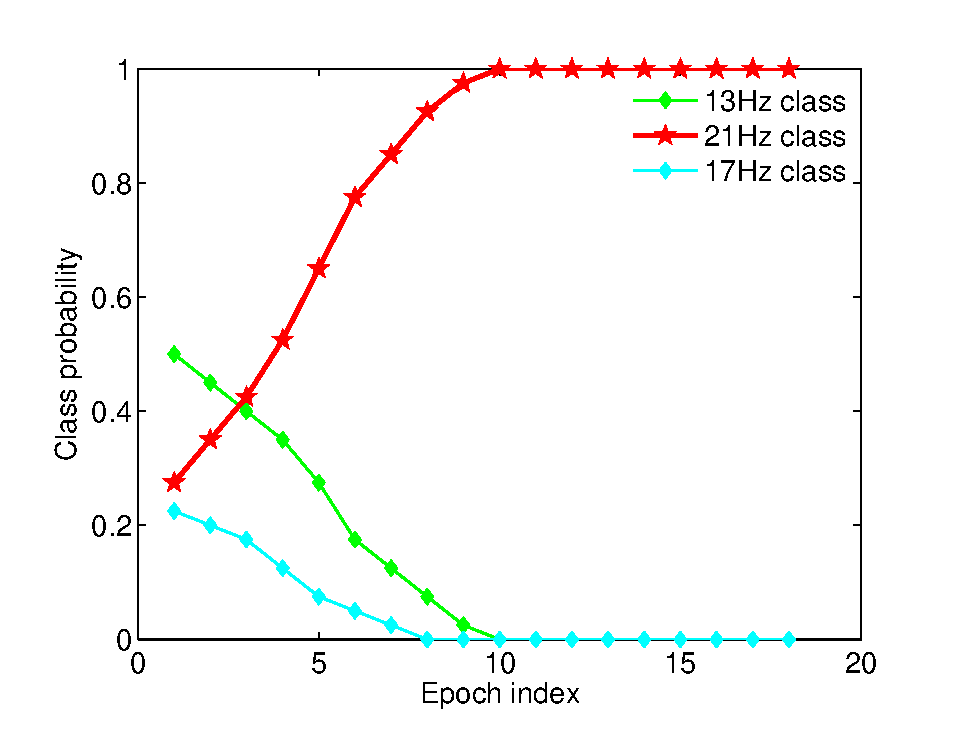
\includegraphics[width=1\textwidth]{Figures/classProb_epochs_s12.eps}
%        \subcaption{ }
%        \label{fig:classProbEpochs}
%        \end{minipage}
%        \begin{minipage}[b]{0.48\linewidth}
%        %\pgfimage[width=1\textwidth]{Figures/classProb_epochs_s12.eps}
%         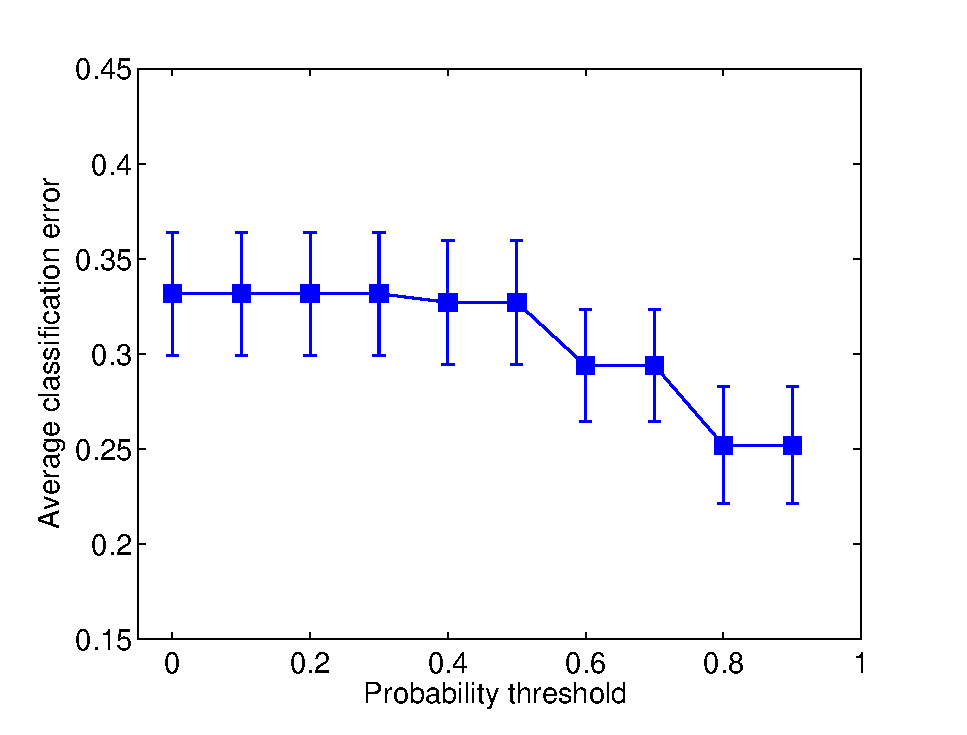
\includegraphics[width=1\textwidth]{Figures/error_probTresh2.eps}
%        \subcaption{ }
%        \label{fig:errorProbTresh}
%        \end{minipage}
%        \begin{minipage}[b]{0.48\linewidth}
%        %\pgfimage[width=1\textwidth]{Figures/classProb_epochs_s12.eps}
%         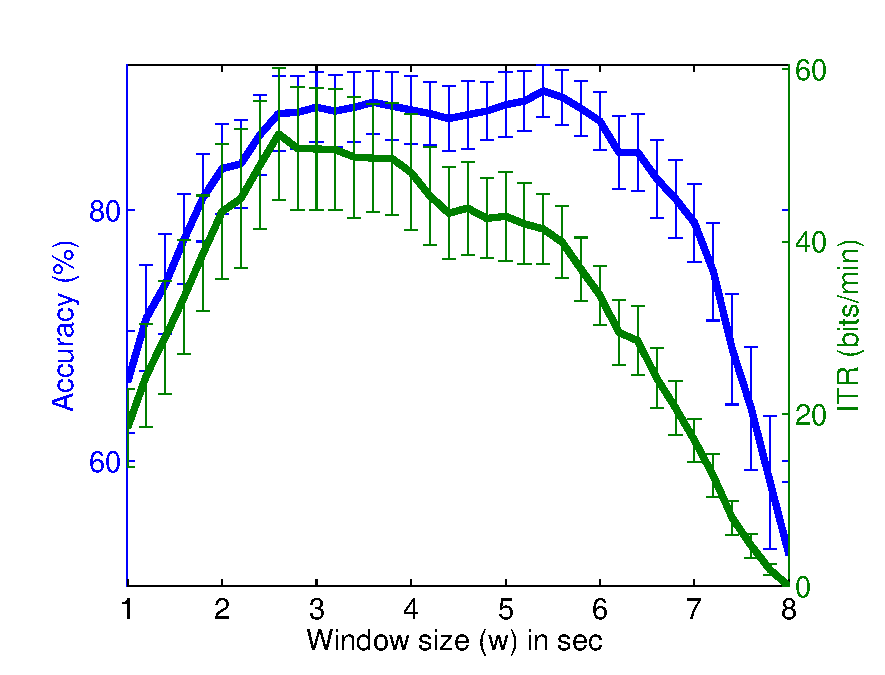
\includegraphics[width=1\textwidth]{Figures/accuracy_tlen.eps}
%        \subcaption{ }
%        \label{fig:accaracy_tlen}
%        \end{minipage}        
%        \caption{Evaluation of the online algorithm parameters.
%            % Online performance analysis as function of online algorithm's parameters.
%            %Analysis of online performance based on the epoch position from the beginning of trial. 
%        \ref{fig:classErrorEpochs} shows the decrease of the average classification error over all subjects during the successive epochs after the beginning of the trial. 
%        \ref{fig:classProbEpochs} is an example taken from the subject with the best performance showing how the probability of the actual class varies with epoch position from beginning of trial.
%        The groundtruth class probability is represented with a thick-and-star line, while other classes probability lines are thin-and-diamond.
%        \ref{fig:errorProbTresh} shows the variation of the average classification error for different probability threshold ($0 \leqslant \pthres < 1$) and its influence on the classifier output (Algorithm \ref{alg:online} step \ref{op3:test_rho}).
%        \ref{fig:accaracy_tlen} shows how the average online performance varies with respect to the epoch size ($\ws$).
%        It shows both the classification accuracy (left y-axis) and the ITR (right y-axis). In \ref{fig:classErrorEpochs}, \ref{fig:errorProbTresh}, and \ref{fig:accaracy_tlen}, \revise{the bars represent the error of the mean i.e. standard deviation divided by the square root of $n-1$, $n$ = number of samples.}}
%\label{fig:probErrorEpochs}.
%\end{figure}
%**********************************************
\begin{figure}[htb!]
\begin{adjustbox}{center}
\resizebox{1.1\textwidth}{!}{
%\centering
\subfigure[]{
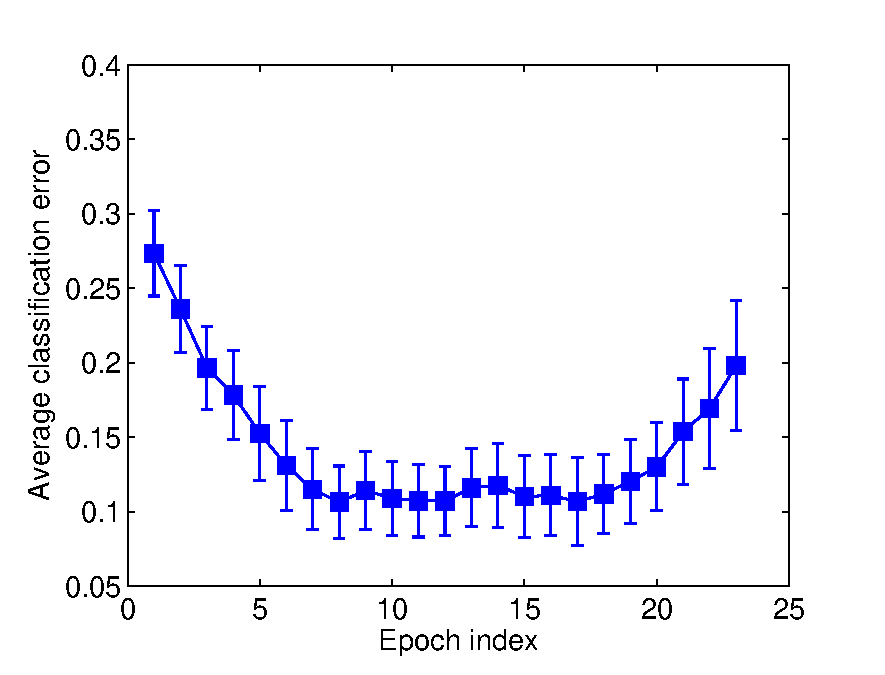
\includegraphics[width=0.5\textwidth]{Figures/classError_epochs.eps}
\label{fig:classErrorEpochs}
}
\subfigure[]{
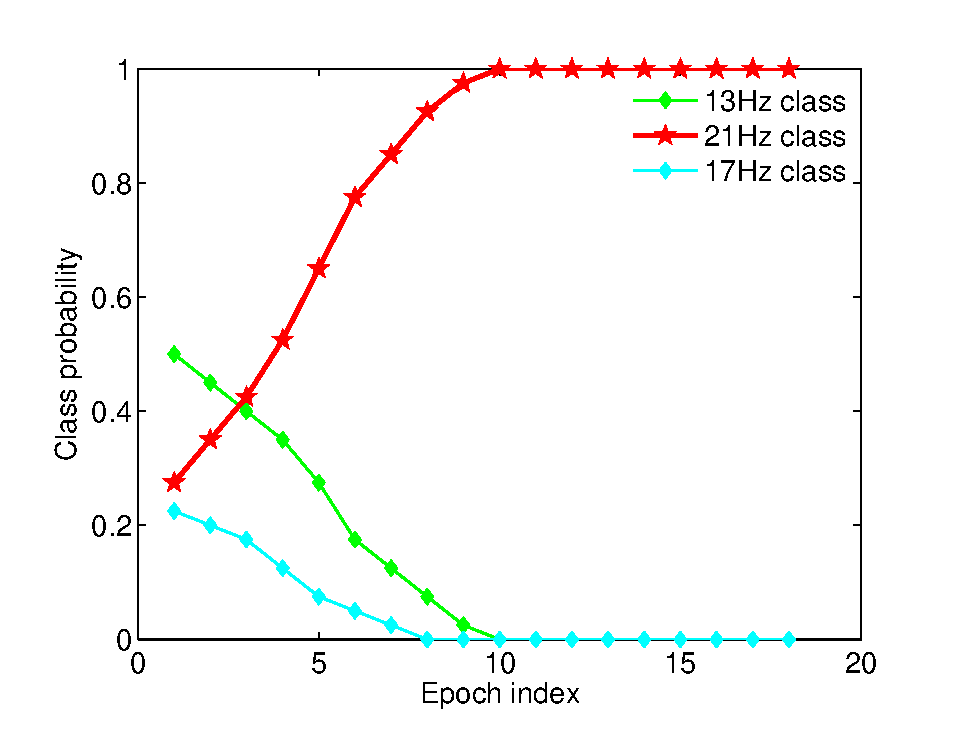
\includegraphics[width=0.5\textwidth]{Figures/classProb_epochs_s12.eps}
\label{fig:classProbEpochs}
}
}
\end{adjustbox}
\begin{adjustbox}{center}
\resizebox{1.1\textwidth}{!}{
\subfigure[]{
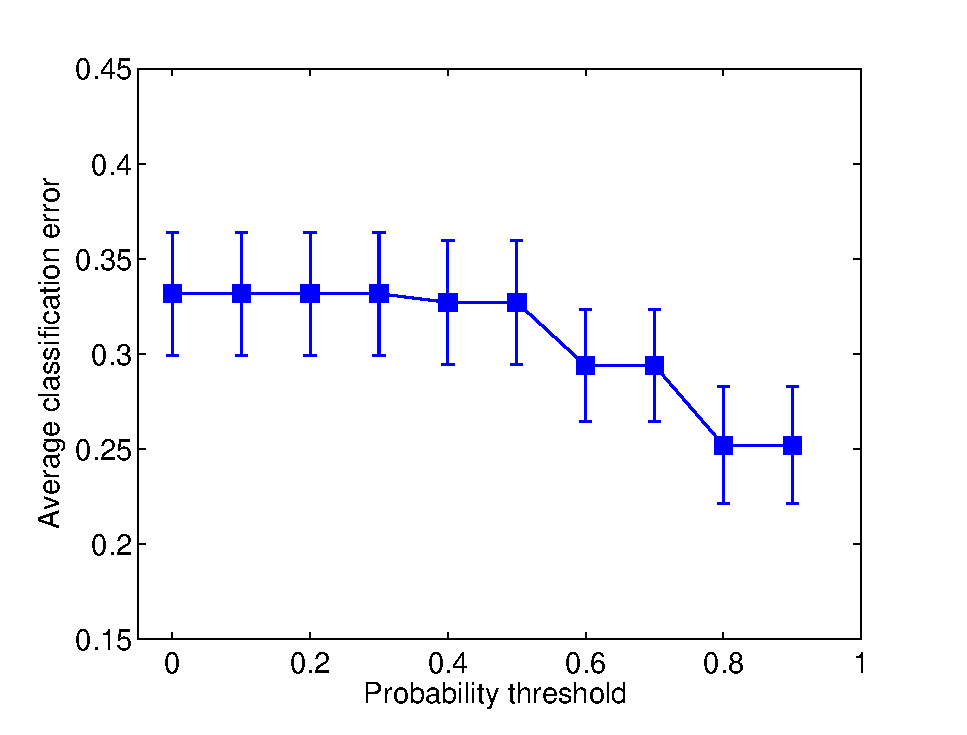
\includegraphics[width=0.5\textwidth]{Figures/error_probTresh2.eps}
\label{fig:errorProbTresh}
}
\subfigure[]{
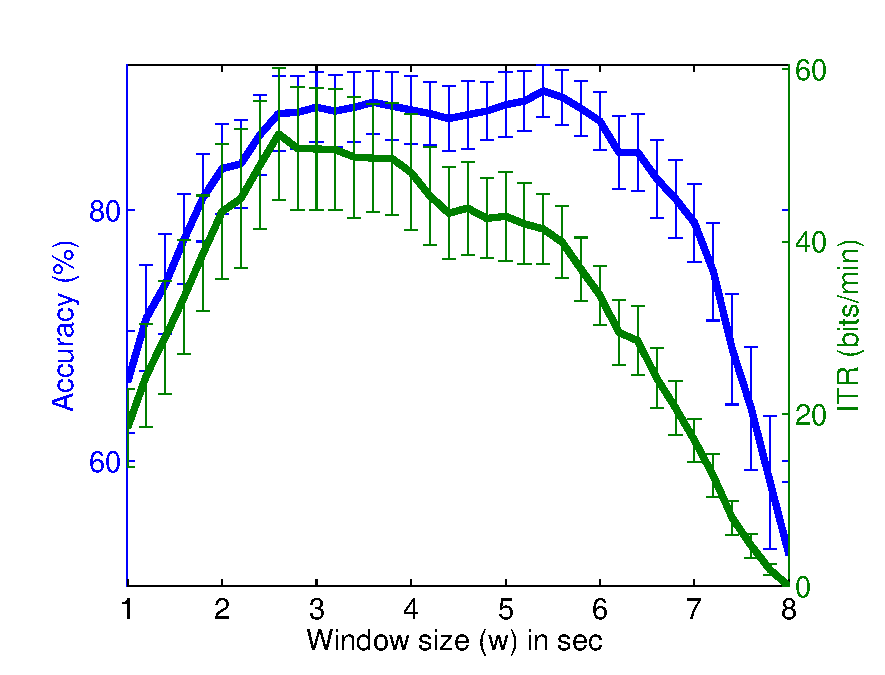
\includegraphics[width=0.5\textwidth]{Figures/accuracy_tlen.eps}
\label{fig:accaracy_tlen}
}
}
\end{adjustbox}
\caption{Evaluation of the online algorithm parameters.
            % Online performance analysis as function of online algorithm's parameters.
            %Analysis of online performance based on the epoch position from the beginning of trial. 
        \ref{fig:classErrorEpochs} shows the decrease of the average classification error over all subjects during the successive epochs after the beginning of the trial. 
        \ref{fig:classProbEpochs} is an example taken from the subject with the best performance showing how the probability of the actual class varies with epoch position from beginning of trial.
        The groundtruth class probability is represented with a thick-and-star line, while other classes probability lines are thin-and-diamond.
        \ref{fig:errorProbTresh} shows the variation of the average classification error for different probability threshold ($0 \leqslant \pthres < 1$) and its influence on the classifier output (Algorithm \ref{alg:online} step \ref{op3:test_rho}).
        \ref{fig:accaracy_tlen} shows how the average online performance varies with respect to the epoch size ($\ws$).
        It shows both the classification accuracy (left y-axis) and the ITR (right y-axis). In \ref{fig:classErrorEpochs}, \ref{fig:errorProbTresh}, and \ref{fig:accaracy_tlen}, the bars represent the error of the mean i.e. standard deviation divided by the square root of $n-1$, $n$ = number of samples.}
\label{fig:probErrorEpochs}
\end{figure}

%Equation~\eqref{eq:dist_vec} is derived from the observation of Figure~\ref{fig:class_path_s17}. 
The observation of Figure~\ref{fig:class_path_s17} provides a visualisation of the principle guiding the online implementation of Equation~\eqref{eq:dist_vec}.
This figure shows the trajectory on the tangent space taken by covariance matrices during a 4-class SSVEP experiment, and how they are classified epoch by epoch. 
It can be seen (encircled in Figure~\ref{fig:class_path1_s17}) that a change in the SSVEP stimulus might not be detected instantaneously by the classifier. 
The trials are erroneously attributed with confidence to the previous class.

%\begin{figure}[ht!]
%		\centering
%		\begin{minipage}[b]{0.78\linewidth}
%        % 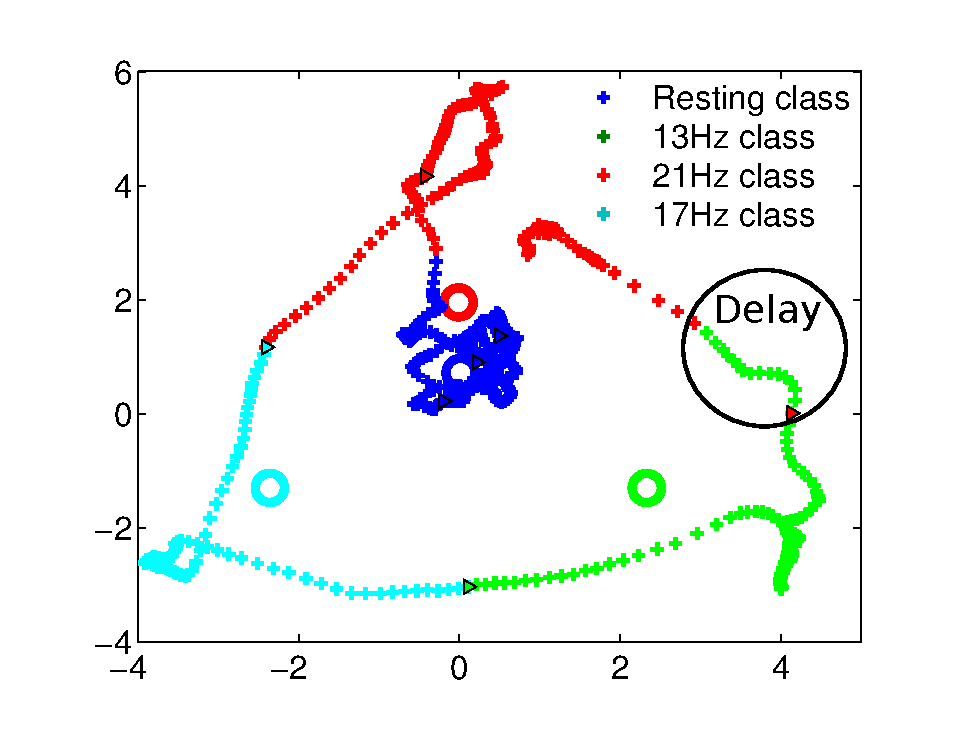
\includegraphics[width=1\textwidth]{Figures/class_path1_s17v3.eps}
%        \pgfimage[width=1\textwidth]{Figures/class_path1_s17v3-eps-converted-to.pdf}
%        \subcaption{ }
%        \label{fig:class_path1_s17}
%      \end{minipage}      
%      \begin{minipage}[b]{0.78\linewidth}
%        \pgfimage[width=1\textwidth]{Figures/class_path2_s17-eps-converted-to.pdf}
%        % 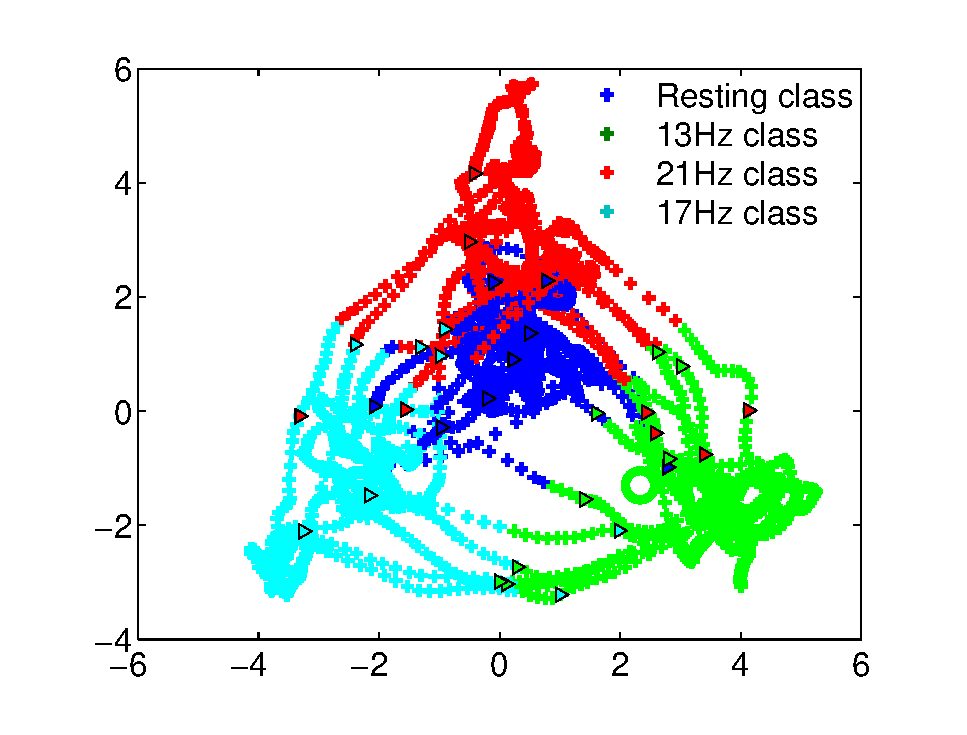
\includegraphics[width=1\textwidth]{Figures/class_path2_s17.eps}
%        \subcaption{ }
%        \label{fig:class_path2_s17}
%        \end{minipage}
%        
%        \caption{Covariance matrices trajectory during a 4-class SSVEP online recording. The circles represent class centers. The triangles mark the beginning in the experiment of a new trial whose class is indicated by the triangle's color. \ref{fig:class_path1_s17} shows the first 7 trials. The first 3 trials are from the resting class, the remaining are respectively class 13Hz, 17Hz, and 21Hz. \ref{fig:class_path2_s17} shows the entire recording. Data are taken from the subject with the highest BCI performance.}
%\label{fig:class_path_s17}
%\end{figure} 
%******************************
\begin{figure}[h!]
%\centering
\begin{adjustbox}{center}
\resizebox{1.2\textwidth}{!}{
\subfigure[]{
\pgfimage[width=0.7\textwidth]{Figures/class_path1_s17v3-eps-converted-to.pdf}
\label{fig:class_path1_s17}
}
\subfigure[]{
\pgfimage[width=0.7\textwidth]{Figures/class_path2_s17-eps-converted-to.pdf}
\label{fig:class_path2_s17}
}
}
\end{adjustbox}
\caption{The covariance matrices trajectory during a 4-class SSVEP online recording. The circles represent class centres. The triangles mark the beginning of the experiment of a new trial whose class is indicated by the triangle's colour. \ref{fig:class_path1_s17} shows the first 7 trials. The first 3 trials are from the resting class, the remaining are respectively class 13 Hz, 17 Hz, and 21 Hz. \ref{fig:class_path2_s17} shows the entire recording. Data are taken from the subject with the highest BCI performance.}
\label{fig:class_path_s17}
\end{figure}


The proposed online algorithm, described in Algorithm~\ref{alg:online}, mitigates this issue and increases the classification accuracy as shown in Table~\ref{tab:res-online}.  %.and \eqref{eq:direction}
The ``Online ($\pocc(\cloutmp)>\pthres$)'' column shows the results of the online algorithm without the curve direction criterion (\textit{i.e.}, without steps 6 to 11), and ``Online (full algo. \ref{alg:online})'' shows the improvement brought by this criterion. 
The performances are in terms of average classification accuracy (acc (\%)), average time taken into the trial before classification (delay (s)), and the ITR (itr (bits/min)).  

\begin{table*}[ht!]
\centering
\ra{1}
\begin{adjustbox}{center}
  \resizebox{1\textwidth}{!}{
  %1CL \resizebox{1.2\textwidth}{!}{
\begin{tabular}{c||c|c|c||c|c|c||c|c|c||}
\cline{2-10}
& \multicolumn{3}{ |c|| }{Online ($\pocc(\cloutmp)>\pthres$) } &\multicolumn{3}{ c|| }{Online (full algo. \ref{alg:online})} &\multicolumn{3}{ c|| }{\onlinepotato} \\ \cline{2-10}
     &   acc(\%) & delay(s) & itr(bpm) &   acc(\%) & delay(s) & itr(bpm) &   acc(\%) & delay(s) & itr(bpm) \\ \hline
  \multicolumn{1}{|c||}{S1} &     68.8 &      0.8 &     26.3 &     77.1 &      1.1 &     27.9 &     77.1 &      1.1 &      27.9 \\ \hline
  \multicolumn{1}{|c||}{S2} &     64.6 &      0.7 &     21.6 &     77.1 &      1.2 &     26.8 &     77.1 &      1.2 &     26.8 \\ \hline
  \multicolumn{1}{|c||}{S3} &     81.2 &      0.7 &     54.3 &     95.8 &      1.0 &     73.0 &     95.8 &      1.0 &     73.0 \\ \hline
  \multicolumn{1}{|c||}{S4} &     83.3 &      0.8 &     53.2 &     91.7 &      1.0 &     58.6 &     95.8 &      1.0 &     69.2 \\ \hline
  \multicolumn{1}{|c||}{S5} &     72.9 &      0.7 &     37.1 &     83.3 &      1.0 &     42.5 &     83.3 &      1.0 &     42.5 \\ \hline
  \multicolumn{1}{|c||}{S6} &     66.7 &      0.7 &     24.5 &     72.9 &      1.1 &     24.3 &     72.9 &      1.1 &     24.3 \\ \hline
  \multicolumn{1}{|c||}{S7} &     93.1 &      0.7 &     89.6 &     98.6 &      0.9 &     87.0 &     98.6 &      0.9 &     86.8 \\ \hline
  \multicolumn{1}{|c||}{S8} &     87.5 &      0.6 &     76.2 &    100.0 &      0.9 &     95.9 &    100.0 &      0.9 &     95.9 \\ \hline
  \multicolumn{1}{|c||}{S9} &     60.4 &      0.7 &     15.7 &     77.1 &      1.2 &     27.6 &     77.1 &      1.2 &     27.6 \\ \hline
 \multicolumn{1}{|c||}{S10} &     64.6 &      0.7 &     21.5 &     87.5 &      1.1 &     45.3 &     87.5 &      1.1 &     45.3 \\ \hline
 \multicolumn{1}{|c||}{S11} &     54.2 &      0.7 &     9.9 &     87.5 &      1.3 &     38.9 &     87.5 &      1.3 &     38.9 \\ \hline
 \multicolumn{1}{|c||}{S12} &     52.5 &      0.7 &     8.0 &     99.2 &      1.2 &     71.7 &     99.2 &      1.2 &     71.8 \\ \hline
\multicolumn{1}{|c||}{\textbf{Mean}} & \textbf{70.8$\pm$13} & \textbf{0.7$\pm$0.0} & \textbf{36.5$\pm$26.3} & \textbf{87.3$\pm$9.8} & \textbf{1.1$\pm$0.1} & \textbf{51.6$\pm$25.1} & \textbf{87.7$\pm$10} & \textbf{1.1$\pm$0.1} & \textbf{52.5$\pm$25.5} \\ \hline
\end{tabular}}}
\end{adjustbox}
\caption{Classification performances (accuracy in \%, delay before valid and confident classification in seconds, and ITR in bits/min) achieved using the online algorithm.
The first column indicates the subjects. The following three columns show the results obtained without the curve direction criterion (Algorithm \ref{alg:online} up to \ref{op3:test_rho}): by stopping at step \ref{op3:test_rho}, $\cloutmp$ is taken to be the valid class. 
The next three columns contain the results of the complete online algorithm.
The last three columns report the results obtained when outliers are removed in the training phase using the Riemannian potato technique described in Section \ref{sec:potato}.}

\label{tab:res-online}
\end{table*}

The curve direction criterion increases the rejection of epochs that could be wrongly classified, it thus significantly increases the classification accuracy of the online algorithm (70.8$\pm$13 \% to 87.3$\pm$9.8\%), while increasing the delay (0.7s to 1.1s) before classification.
When compared to the state-of-the-art offline MDRM, the online curve-based classification yields better results in terms of ITR as the delay before classification is much shorter in the latter than the trial length used in the former; classification outputs are reached faster with the online algorithm. 
%When compared to the state-of-the-art offline MDRM, the online curve-based classification yields better results in terms of classification accuracy, delay before classification, and ITR \textit{i.e.} from 71.51\% to 79.13\%, from 3.6s (or longer, depending on trial length $\dt$) to 1.239s, and from 12.33 to 47.94.
%There is a small drop in classification accuracy from optimized offline (81.27\%) to online (79.13\%) algorithms.
%However, classification outputs are reached faster with the online algorithm.
Moreover, the online algorithm can be applied in both synchronous and asynchronous paradigms, whereas the offline algorithms are limited to synchronous paradigms which provide strongly limited user interaction. 

Last, the impact of the Riemannian potato is analysed. 
A bootstrapping with 50 replications was performed on the offline data to assess the effect of applying the Riemannian potato. 
The results show that for most subjects the results are unchanged when the Riemannian potato is applied: due to the fact that data are recorded in a controlled environment, most of them are thus clean.
It does, however, improve the results of few subjects. 
It was then applied in the training phase of the online application, and a similar observation is made. 
%Table \ref{tab:online-potato} summarizes the results.
We can conclude that the Riemannian potato can be used as a safety guard to ensure that the Riemannian mean used in the MDRM classification scheme is not affected by outliers, especially for BCI used in less controlled environment.

\subsubsection{Online Analysis with Resting Class}

Using the MDRM approach it is possible to identify the resting class. 
In fact, covariance matrices of signals recorded during resting periods can be characterised with their own Riemannian mean.
As such, they can be identified as any other class using the MDRM approach.
The state-of-the-art methods, \citep{lin_frequency_2006} and \citep{nakanishi_high-speed_2014}, are both based on CCA where a reference signal is needed.
These methods do not handle resting class, since there is no reference signal for them.
In this section, the performance of the proposed approach including the identification of the resting class is presented.
%The parameters of the online algorithm with the identification of the resting class are analyzed and shown in Figure~\ref{fig:online-analysis-4class}. 
Table~\ref{tab:res-online-resting} summarises the classifier performance in the same format as Table~\ref{tab:res-online}, in terms of classification accuracy, delay before valid classification and ITR.
Like in Table~\ref{tab:res-online}, the best performance is achieved  by the complete online algorithm preceded with outlier removal with the Riemannian potatoes (\textit{i.e.} \emph{\onlinepotato}).
The identification of the resting class induces a drop of the overall classification accuracy by 8.2\%, and a drop of ITR from 52.5$\pm$25.5 to 49.2$\pm$18.2.

The effect of the resting class is seen with more details in Figure~\ref{fig:cm-roc}. 
Figure~\ref{fig:confusion-matrix} shows the classification confusion matrix. 
There are few misclassifications between SSVEP classes compared to the misclassifications between the resting class and any SSVEP class: the largest percentages are located in the first row and the first column, apart from the diagonal block. 
Figure~\ref{fig:roc-curve} displays a ROC curve showing how the classifier performs in discriminating each class versus the others depending on the value of the $\pthres$ parameter. 
On this ROC curve, the performance of the \onlinepotato{} algorithm is indicated in terms of False Positive Rate (FPR) and True Positive Rate (TPR).

Confirming the observation from the confusion matrix, the ROC curve indicates that the resting is the most prone to false positive.
Despite the drop in performance, the identification of resting class is crucial for online BCI setup, allowing the subject to use the system at his own pace. 

\begin{table*}[ht!]
\centering
\ra{1}
\begin{adjustbox}{center}
\resizebox{1.2\textwidth}{!}{
\begin{tabular}{c|c|c|c||c|c|c||c|c|c||}
\cline{2-10}
& \multicolumn{3}{ |c|| }{Online ($\pocc(\cloutmp)>\pthres$) } &\multicolumn{3}{ c|| }{Online (full algo. \ref{alg:online})} &\multicolumn{3}{ c|| }{\onlinepotato} \\ \cline{2-10}
     &   acc(\%) & delay(s) & itr(bpm) &   acc(\%) & delay(s) & itr(bpm) &   acc(\%) & delay(s) & itr(bpm) \\ \hline
  \multicolumn{1}{|c|}{S1} &     67.2 &      0.7 &     37.6 &     71.4 &      1.1 &     32.4 &     71.4 &      1.1 &     32.4 \\ \hline
  \multicolumn{1}{|c|}{S2} &     78.1 &      0.7 &     59.0 &     75.0 &      1.0 &     39.2 &     75.0 &      1.0 &     39.2 \\ \hline 
  \multicolumn{1}{|c|}{S3} &     89.1 &      0.8 &     85.2 &     89.1 &      1.0 &     67.6 &     89.1 &      1.0 &     67.6 \\ \hline
  \multicolumn{1}{|c|}{S4} &     75.0 &      0.7 &     52.2 &     75.0 &      0.9 &     42.9 &     75.0 &      0.9 &     43.4 \\ \hline
  \multicolumn{1}{|c|}{S5} &     71.9 &      0.7 &     46.7 &     70.3 &      1.1 &     31.0 &     70.3 &      1.1 &     31.0 \\ \hline
  \multicolumn{1}{|c|}{S6} &     87.5 &      0.8 &     80.2 &     87.3 &      1.1 &     58.7 &     87.3 &      1.1 &     58.7 \\ \hline
  \multicolumn{1}{|c|}{S7} &     84.4 &      0.7 &     76.3 &     85.4 &      1.0 &     62.5 &     88.5 &      1.0 &     69.1 \\ \hline
  \multicolumn{1}{|c|}{S8} &     85.9 &      0.8 &     76.4 &     89.1 &      1.0 &     68.1 &     89.1 &      1.0 &     68.1 \\ \hline
  \multicolumn{1}{|c|}{S9} &     67.2 &      0.7 &     37.2 &     75.0 &      1.0 &     39.6 &     76.6 &      1.1 &     40.3 \\ \hline
 \multicolumn{1}{|c|}{S10} &     62.5 &      0.7 &     30.3 &     69.5 &      1.0 &     32.0 &     69.5 &      1.0 &     32.0 \\ \hline
 \multicolumn{1}{|c|}{S11} &     59.4 &      0.8 &     23.5 &     68.8 &      1.1 &     29.1 &     68.8 &      1.1 &     29.1 \\ \hline
 \multicolumn{1}{|c|}{S12} &     69.4 &      0.7 &    44.8 &     93.8 &      1.0 &     79.4 &     93.8 &      1.0 &     79.9 \\ \hline
\multicolumn{1}{|c|}{\textbf{Mean}} & \textbf{74.8$\pm$10.2} & \textbf{0.7$\pm$0.0} & \textbf{54.1$\pm$21.0} & \textbf{79.1$\pm$9.1} & \textbf{1.0$\pm$0.1} & \textbf{48.6$\pm$17.6} & \textbf{79.5$\pm$9.3} & \textbf{1.0$\pm$0.1} & \textbf{49.2$\pm$18.2} \\ \hline
\end{tabular}}
\end{adjustbox}
\caption{This table summarises the performance achieved with the online algorithm with resting class identification, as in Table~\ref{tab:res-online}.
%The first column indicates the subjects. The following three columns show the results obtained without the curve direction criterion (Algorithm \ref{alg:online} up to \ref{op3:test_rho}): by stopping at step \ref{op3:test_rho}, $\cloutmp$ is taken to be the valid class. 
%The next three columns contain the results of the the complete online algorithm.
%The last three columns report the results obtain when outliers are removed in the training phase using the Riemannian potato technique described in Section \ref{sec:potato}.
}

%\caption{Average classification accuracy for each subject and time delay, from beginning of trial $t_0$, before valid classification output. The results obtained when using the cue onset $t_0$ as time reference and a fixed 2-seconds delay (synchronous) are compared to the results where no time reference is used (asynchronous), and enhanced by $\disvec_j$ (asynchronous + $\disvec_j$).}
\label{tab:res-online-resting}
\end{table*}

%\begin{figure*}[ht!]
%		\centering
%		\begin{minipage}[b]{0.48\linewidth}
%         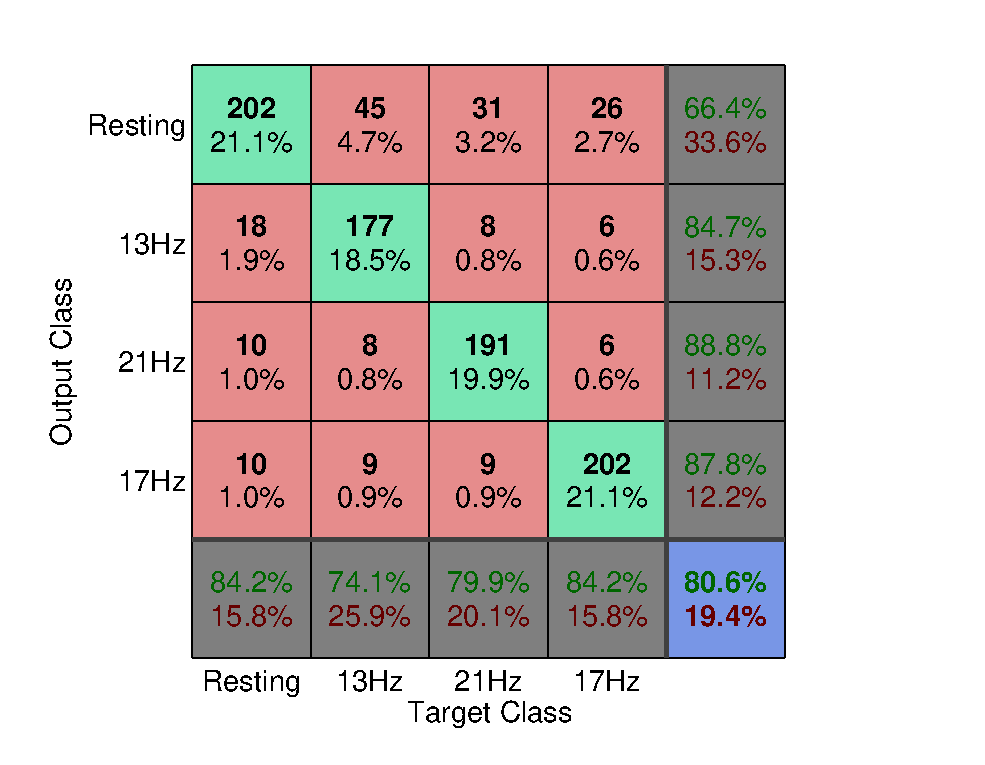
\includegraphics[width=1\textwidth]{Figures/confusionMatrix.eps}
%        %\pgfimage[width=1\textwidth]{Figures/classError_epochs.eps}
%        \subcaption{ }
%        \label{fig:confusion-matrix}
%      \end{minipage}      
%      \begin{minipage}[b]{0.48\linewidth}
%        %\pgfimage[width=1\textwidth]{Figures/classProb_epochs_s12.eps}
%         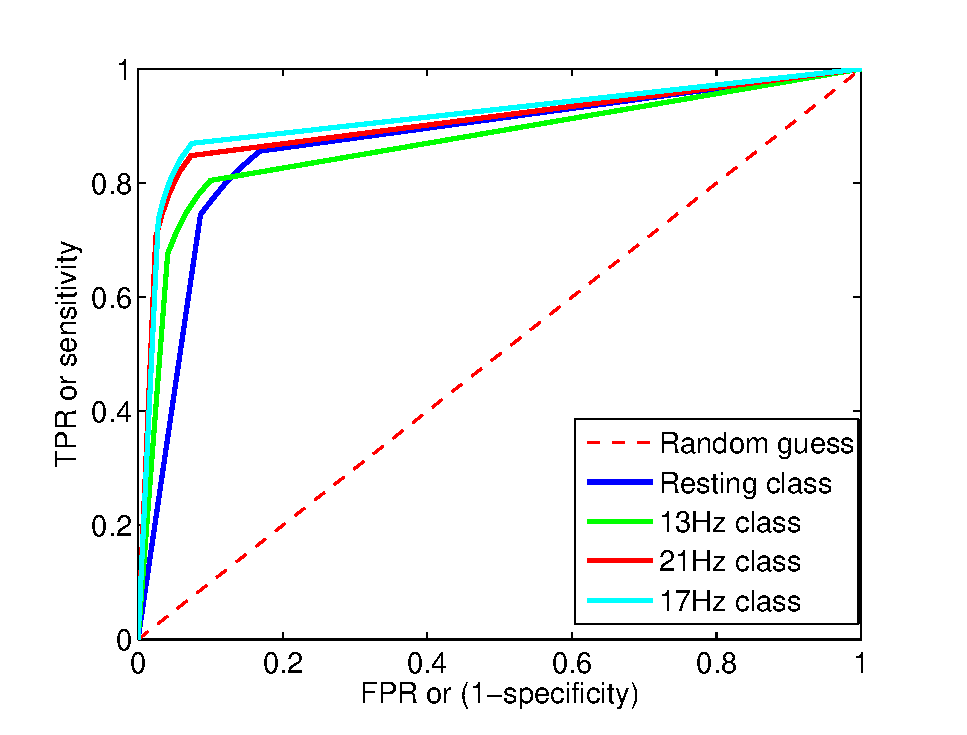
\includegraphics[width=1\textwidth]{Figures/roc.eps}
%        \subcaption{ }
%        \label{fig:roc-curve}
%        \end{minipage}        
%        \caption{(a) Confusion matrix for $K=4$ classes with \onlinepotato.  %\ref{fig:confusion-matrix}
%           (b): ROC curve indicating the influence of the $\pthres$ parameter. %\ref{fig:roc-space}
%         }
%       \label{fig:cm-roc}
%%1CL \end{figure}
%\end{figure*}
%***************************************
\begin{figure}[h!]
%\centering
\begin{adjustbox}{center}
\resizebox{1.2\textwidth}{!}{
\subfigure[]{
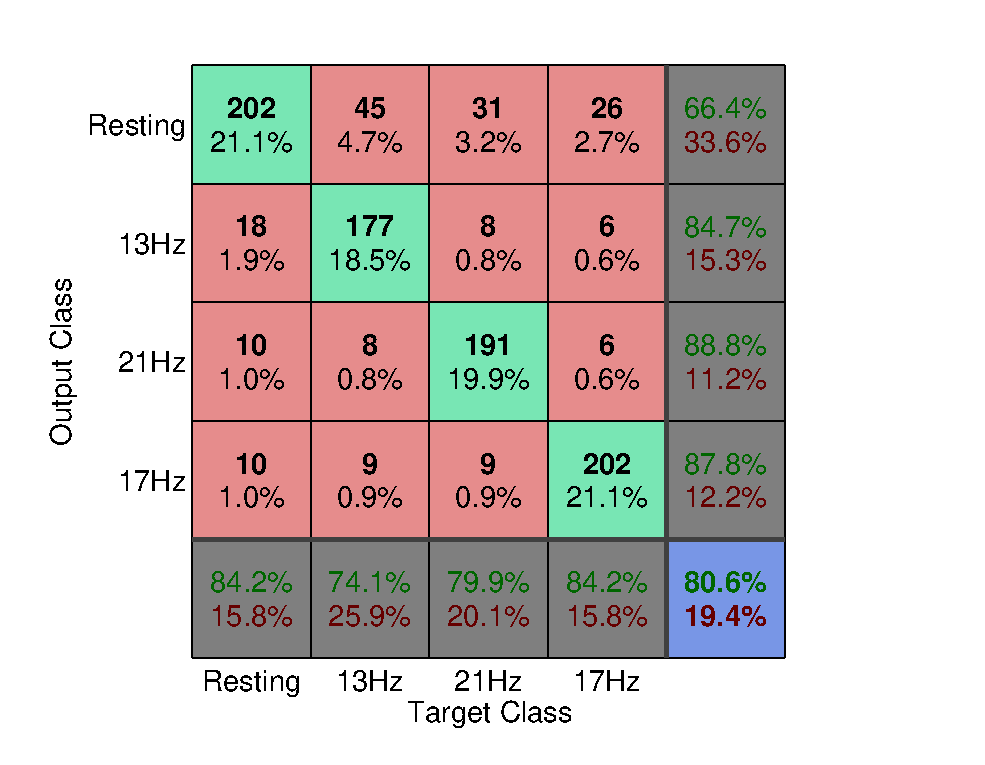
\includegraphics[width=0.6\textwidth]{Figures/confusionMatrix.eps}
\label{fig:confusion-matrix}
}
\subfigure[]{
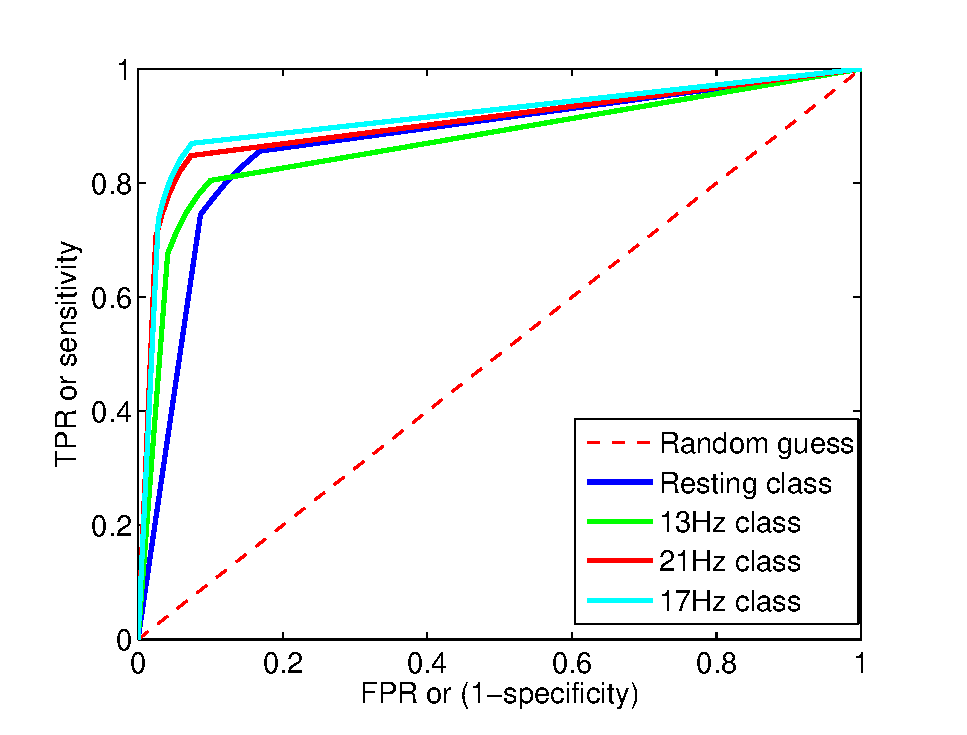
\includegraphics[width=0.6\textwidth]{Figures/roc.eps}
\label{fig:roc-curve}
}
}
\end{adjustbox}
\caption{(a) Confusion matrix for $K=4$ classes with \onlinepotato. 
(b): ROC curve indicating the influence of the $\pthres$ parameter. %\ref{fig:roc-space}
}
\label{fig:cm-roc}
\end{figure}


\section{Conclusion}
\label{sec:riem-conclusion}

%\remSyl{Each TBME article must include a conclusion section elaborating the major findings and significance of the work, as well as applications. This section should not exceed 300 words.}
This chapter investigated the efficiency of Riemannian geometry when dealing with covariance matrices as classification features.
Existing covariance matrix estimators were investigated and their robustness was assessed on multichannel SSVEP signals to ensure that the obtained matrices are accurate estimates of data covariance, are well conditioned, and verify the positive-definiteness property. 
The Sch\"afer shrinkage estimator was found to be the best as it yielded the highest classification accuracy with the MDRM algorithm.
The chapter demonstrated the interest in moving from Euclidean to Riemannian geometry in the design of machine learning algorithms applied to EEG signal and SSVEP in particular. 
Various distances and divergences as well as their corresponding means were presented and evaluated. 
Riemannian metric/divergences and their means are shown to be more appropriate on the structure of SPD matrices, and yield better results than their Euclidean counterparts in machine learning algorithms for classification.
A novel algorithm based on MDRM, enhanced by class probability and the curve direction in the space of covariance EEG signals, was introduced and applied on a SSVEP classification task for a 4-class brain-computer interface. 

The MDRM approach is first analysed in an offline classification setup.
To prevent the effect of noisy signals on the MDRM approach, outliers in the training set of are removed using a modified version of the \textit{Riemannian potato}.  
This approach is compared to two CCA-based state-of-the-art methods. % are implemented for comparison purposes. 
The results show that offline MDRM achieves better classification performances than any of the CCA-based methods.

In the online setup, the proposed online algorithm enhances the stability of the BCI system, balancing between classification speed and prediction accuracy. 
The evaluation of the classification confidence over several epochs mitigates the short term perturbations in the experimental conditions and the attentional variations of the subject.
The curve direction overcomes the misclassification of EEG trials that are still synchronised with past stimuli frequencies at classification time.

Unlike the CCA-based state-of-the-art methods considered in this work, the proposed online algorithm is capable of identifying the resting periods during an online EEG recording. 
These resting periods are considered as an additional class in the classification task.

All these contributions help to pave the way towards BCI used in non-controlled, assistive environment. 